\newpage
\section{Results and Discussion}
\label{sec:results}

\subsection{Results Overview}
\label{subsec:results_overview}
This chapter presented the processed experimental results for Heliotron~J discharges \#88653 (primary shot) and \#88654 (replicate shot), evaluated side by side and never pooled into combined averages or joint $p$-values. The analysis followed the three specific objectives: spectral and spatial mode characterization across heating phases and ECH switch-off (Section~\ref{subsec:obj1}), lagged correlation and frequency-scaling evaluation against heating proxies (Section~\ref{subsec:obj2}), and auto-bicoherence testing for three-wave coupling (Section~\ref{subsec:obj3}). All reported values represented conditioned diagnostic outputs accompanied by confidence intervals or effective sample sizes ($N_{\mathrm{eff}}$), alongside explicit diagnostic and estimator limitations.


\subsection{Objective 1 -- Spectral Properties, Temporal Evolution, and Dominant Modes}
\label{subsec:obj1}

\subsubsection{Mode Detection and Structure}
\label{subsubsec:obj1_detection}

\begin{figure}[H]
  \centering
  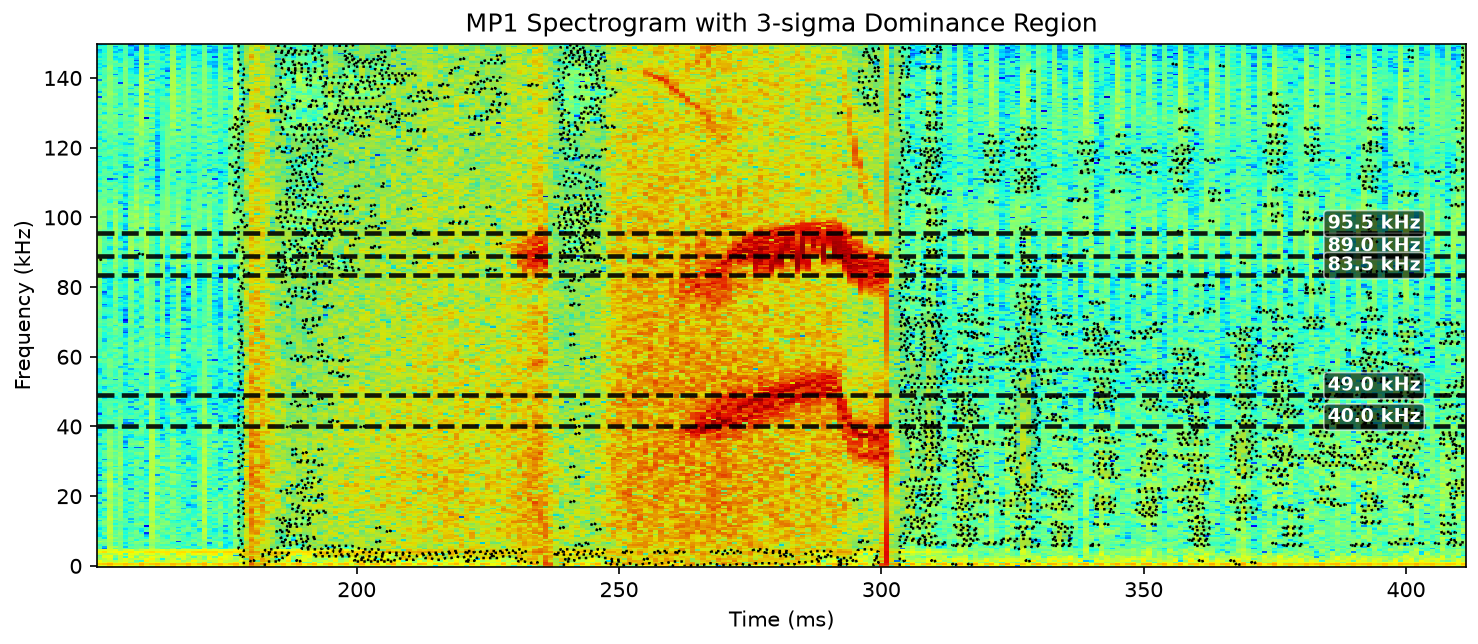
\includegraphics[width=0.86\textwidth]{Images/obj1_mode_identification/panels/mhd_analysis_objective1_88653_panel1_mp1_spectrogram_with_3_sigma_dominance_r.png}
  \caption[Mirnov MP1 spectrogram with statistical dominance threshold]{Mirnov MP1 PSD spectrogram ($500~\mathrm{Hz}$ resolution) with $3\sigma$ dominance contours over $150.0\text{--}350.0~\mathrm{ms}$ in shot \#88653.}
  \label{fig:obj1_spectrogram}
\end{figure}
Figure~\ref{fig:obj1_spectrogram} showed the MP1 STFT spectrogram for shot \#88653, isolating fluctuations that exceeded the $3\sigma$ pre-plasma noise baseline for $\geq 2~\mathrm{ms}$. After a brief burst near $230\text{--}236~\mathrm{ms}$, two dominant bands persisted across late $\mathrm{ECH}+\mathrm{NBI}$ and $\mathrm{NBI}$-only heating ($259.1\text{--}300.4~\mathrm{ms}$): the primary mode shifted from a mean of $87.5~\mathrm{kHz}$ to $86.5~\mathrm{kHz}$ across ECH switch-off, while the secondary mode dropped from $45.8~\mathrm{kHz}$ to $39.7~\mathrm{kHz}$. Because MP1 sampled a single-point edge location without radial resolution, internal localization and 3D coupling were established by cross-correlating the 16 ECE channels against all 18 Mirnov coils (Section~\ref{subsubsec:obj1_radial}).

\begin{figure}[H]
  \centering
  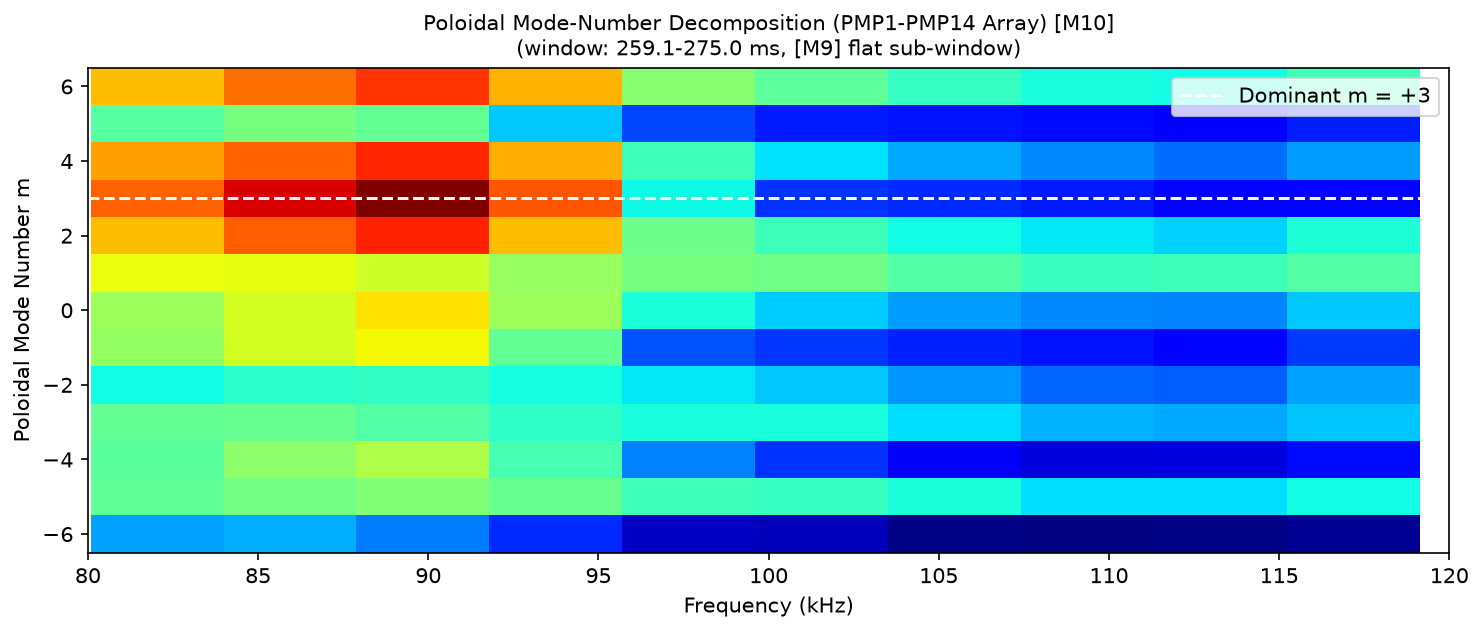
\includegraphics[width=0.85\textwidth]{Images/obj2_dynamics_and_structure/panels/mhd_analysis_objective2_structure_88653_80_120kHz_panel3_poloidal_mode_number_decomposition_pmp1.png}
  \caption[NUDFT poloidal mode decomposition for the primary mode]{NUDFT poloidal mode spectrum across PMP1--PMP14 for $80\text{--}120~\mathrm{kHz}$ over $259.1\text{--}275.0~\mathrm{ms}$ in shot \#88653.}
  \label{fig:obj1_poloidal_m}
\end{figure}
Figure~\ref{fig:obj1_poloidal_m} displayed the NUDFT poloidal mode decomposition across coils PMP1--PMP14 (after PMP1--PMP4 polarity correction) for the primary band ($80$--$120~\mathrm{kHz}$) over the $259.1$--$275.0~\mathrm{ms}$ flat-frequency sub-window of shot \#88653. Power concentrated at $84\text{--}95~\mathrm{kHz}$ along $m = +3$, while unequal poloidal coil spacing introduced residual sidelobe power into $m = +2, +4$ that required phase-concentration verification.

\begin{figure}[H]
  \centering
  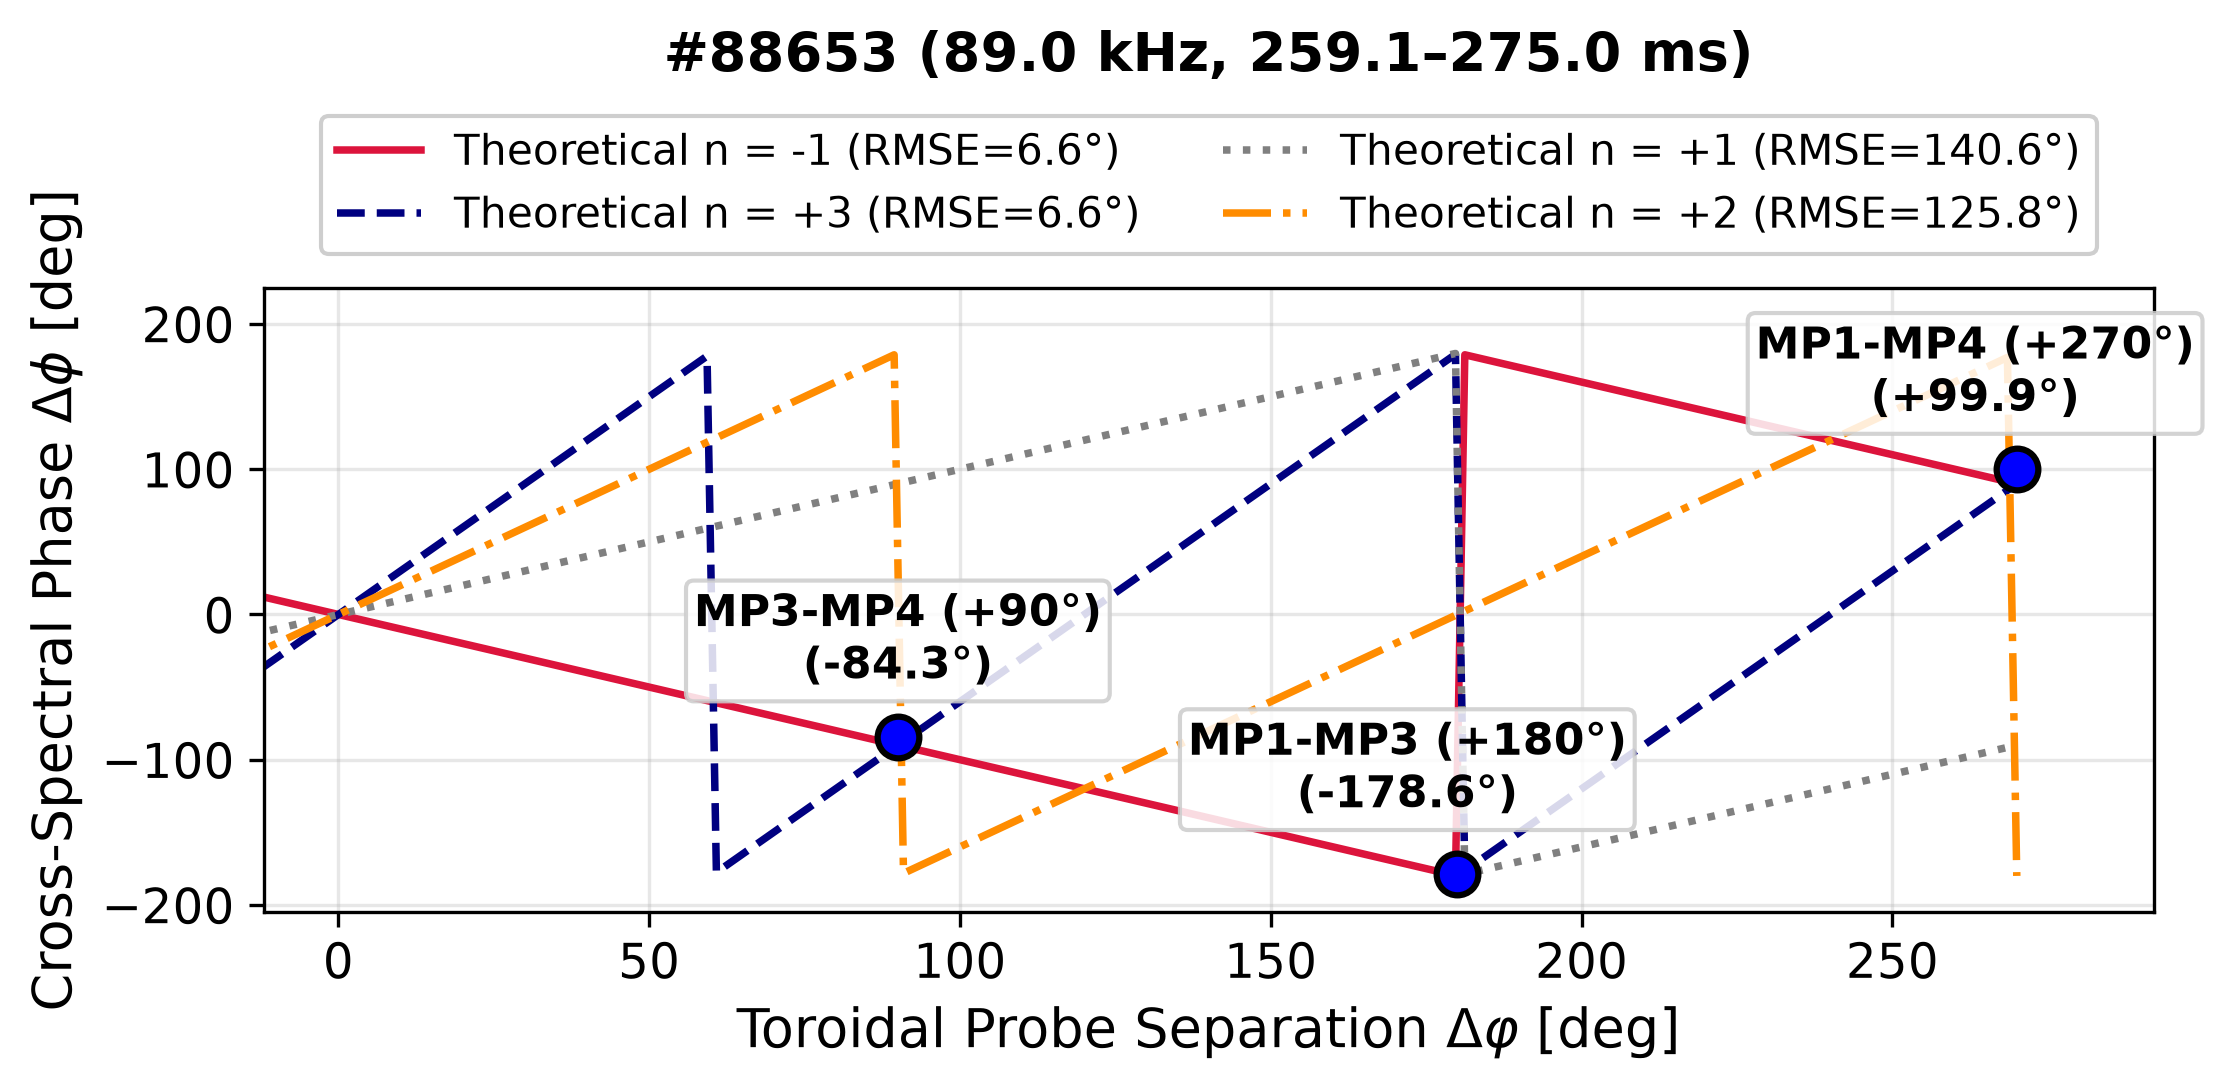
\includegraphics[width=0.85\textwidth]{Images/obj1_mode_identification/panels/mhd_primary_mode_toroidal_n_shot_88653_panel2_measured_phase_vs_theoretical_toroidal_p.png}
  \caption[Cross-probe phase versus toroidal angle for the primary mode]{Cross-spectral phase $\Delta\phi$ versus toroidal separation $\Delta\varphi$ at $89~\mathrm{kHz}$ ($259.1\text{--}275.0~\mathrm{ms}$, \#88653), fitting $n \equiv -1 \pmod 4$.}
  \label{fig:obj1_toroidal_n}
\end{figure}
Figure~\ref{fig:obj1_toroidal_n} compared the cross-spectral phase differences among coplanar coils MP1, MP3, and MP4 ($\Delta\phi = -84.3^\circ$ at $\Delta\varphi = +90^\circ$, $-178.6^\circ$ at $+180^\circ$, and $+99.9^\circ$ at $+270^\circ$) against candidate toroidal mode numbers for the $89~\mathrm{kHz}$ mode. The measured phases matched the degenerate aliases $n = -1$ and $n = +3$ ($\mathrm{RMSE} = 6.6^\circ$), rejecting $n = +1$ ($140.6^\circ$) and $n = +2$ ($125.8^\circ$). With three coplanar toroidal probes, the toroidal mode number was uniquely resolved modulo~4 ($n \equiv -1 \pmod 4$, \emph{supported}).

\begin{table}[H]
\centering
\footnotesize
\setlength{\tabcolsep}{2.6pt}
\renewcommand{\arraystretch}{1.15}
\caption[Spatial mode structure across heating phases and slices]{Spatial mode structure across heating phases and slices.}
\label{tab:mode_structure}
\sbox0{%
\begin{tabular}{llcccclccc}
\toprule
Band & Phase & \shortstack{$f$\\(kHz)} & \shortstack{$m$\\(-)} & \shortstack{$r_{\rm circ}$\\(-)} & \shortstack{Pol.\\Err. ($^\circ$)} & Label & \shortstack{Tor. $n$\\(mod 4, -)$^\dagger$} & \shortstack{Tor.\\RMSE ($^\circ$)} & \shortstack{Radial $\rho$ (-)\\(ECE12/13)} \\
\midrule
Secondary & ECH+NBI & 48.8 & $+1 \wedge +12$ & 0.832 & 24.9 & \emph{supported} & $-1$ & 22.7 & $0.29\text{--}0.47$ \\
Secondary & NBI only & 41.0 & $+1 \wedge +12$ & 0.854 & 25.7 & \emph{supported} & $-1$ & 19.3 & $0.29\text{--}0.47$ \\
Primary & ECH+NBI & 89.8 & $+3$ & 0.882 & 26.7 & \emph{supported} & $-1$ & 5.2 & $0.29\text{--}0.47$ \\
Primary & NBI only & 85.9 & $+3$ & 0.902 & 22.2 & \emph{supported} & $-1$ & 6.7 & $0.29\text{--}0.47$ \\
\shortstack[l]{Primary slice\\\#88653} & \shortstack[l]{post-transition\\291.4--291.8 ms} & -- & $+1$ & 0.608 & 65.0 & \emph{unresolved} & -- & -- & -- \\
\shortstack[l]{Primary slice\\\#88654} & \shortstack[l]{post-transition\\292.0--293.0 ms} & -- & $+3$ & 0.951 & 15.8 & \emph{supported} & -- & -- & -- \\
\bottomrule
\end{tabular}}
\ifdim\wd0>\textwidth\resizebox{\textwidth}{!}{\usebox0}\else\usebox0\fi
\par\smallskip Rows 1--4 correspond to shot \#88653; slices were analyzed individually. $^\dagger$Toroidal fit yields $n \bmod 4$ only (from three toroidal probes). \emph{Supported} requires $r_{\rm circ}\ge 0.70$ and mean poloidal error $\le 45^\circ$; ECE12/13 were calibrated via 3D \textsc{TRAVIS}. Post-transition slices were evaluated at 1~MHz using 256-sample segments with 192-sample overlap ($3$ and $12$ segments for $0.4$~ms and $1.0$~ms windows, respectively); ``--'' indicates parameters omitted in these single-frequency ($87$~kHz) short-window analyses.
\end{table}


\begin{figure}[H]
  \centering
  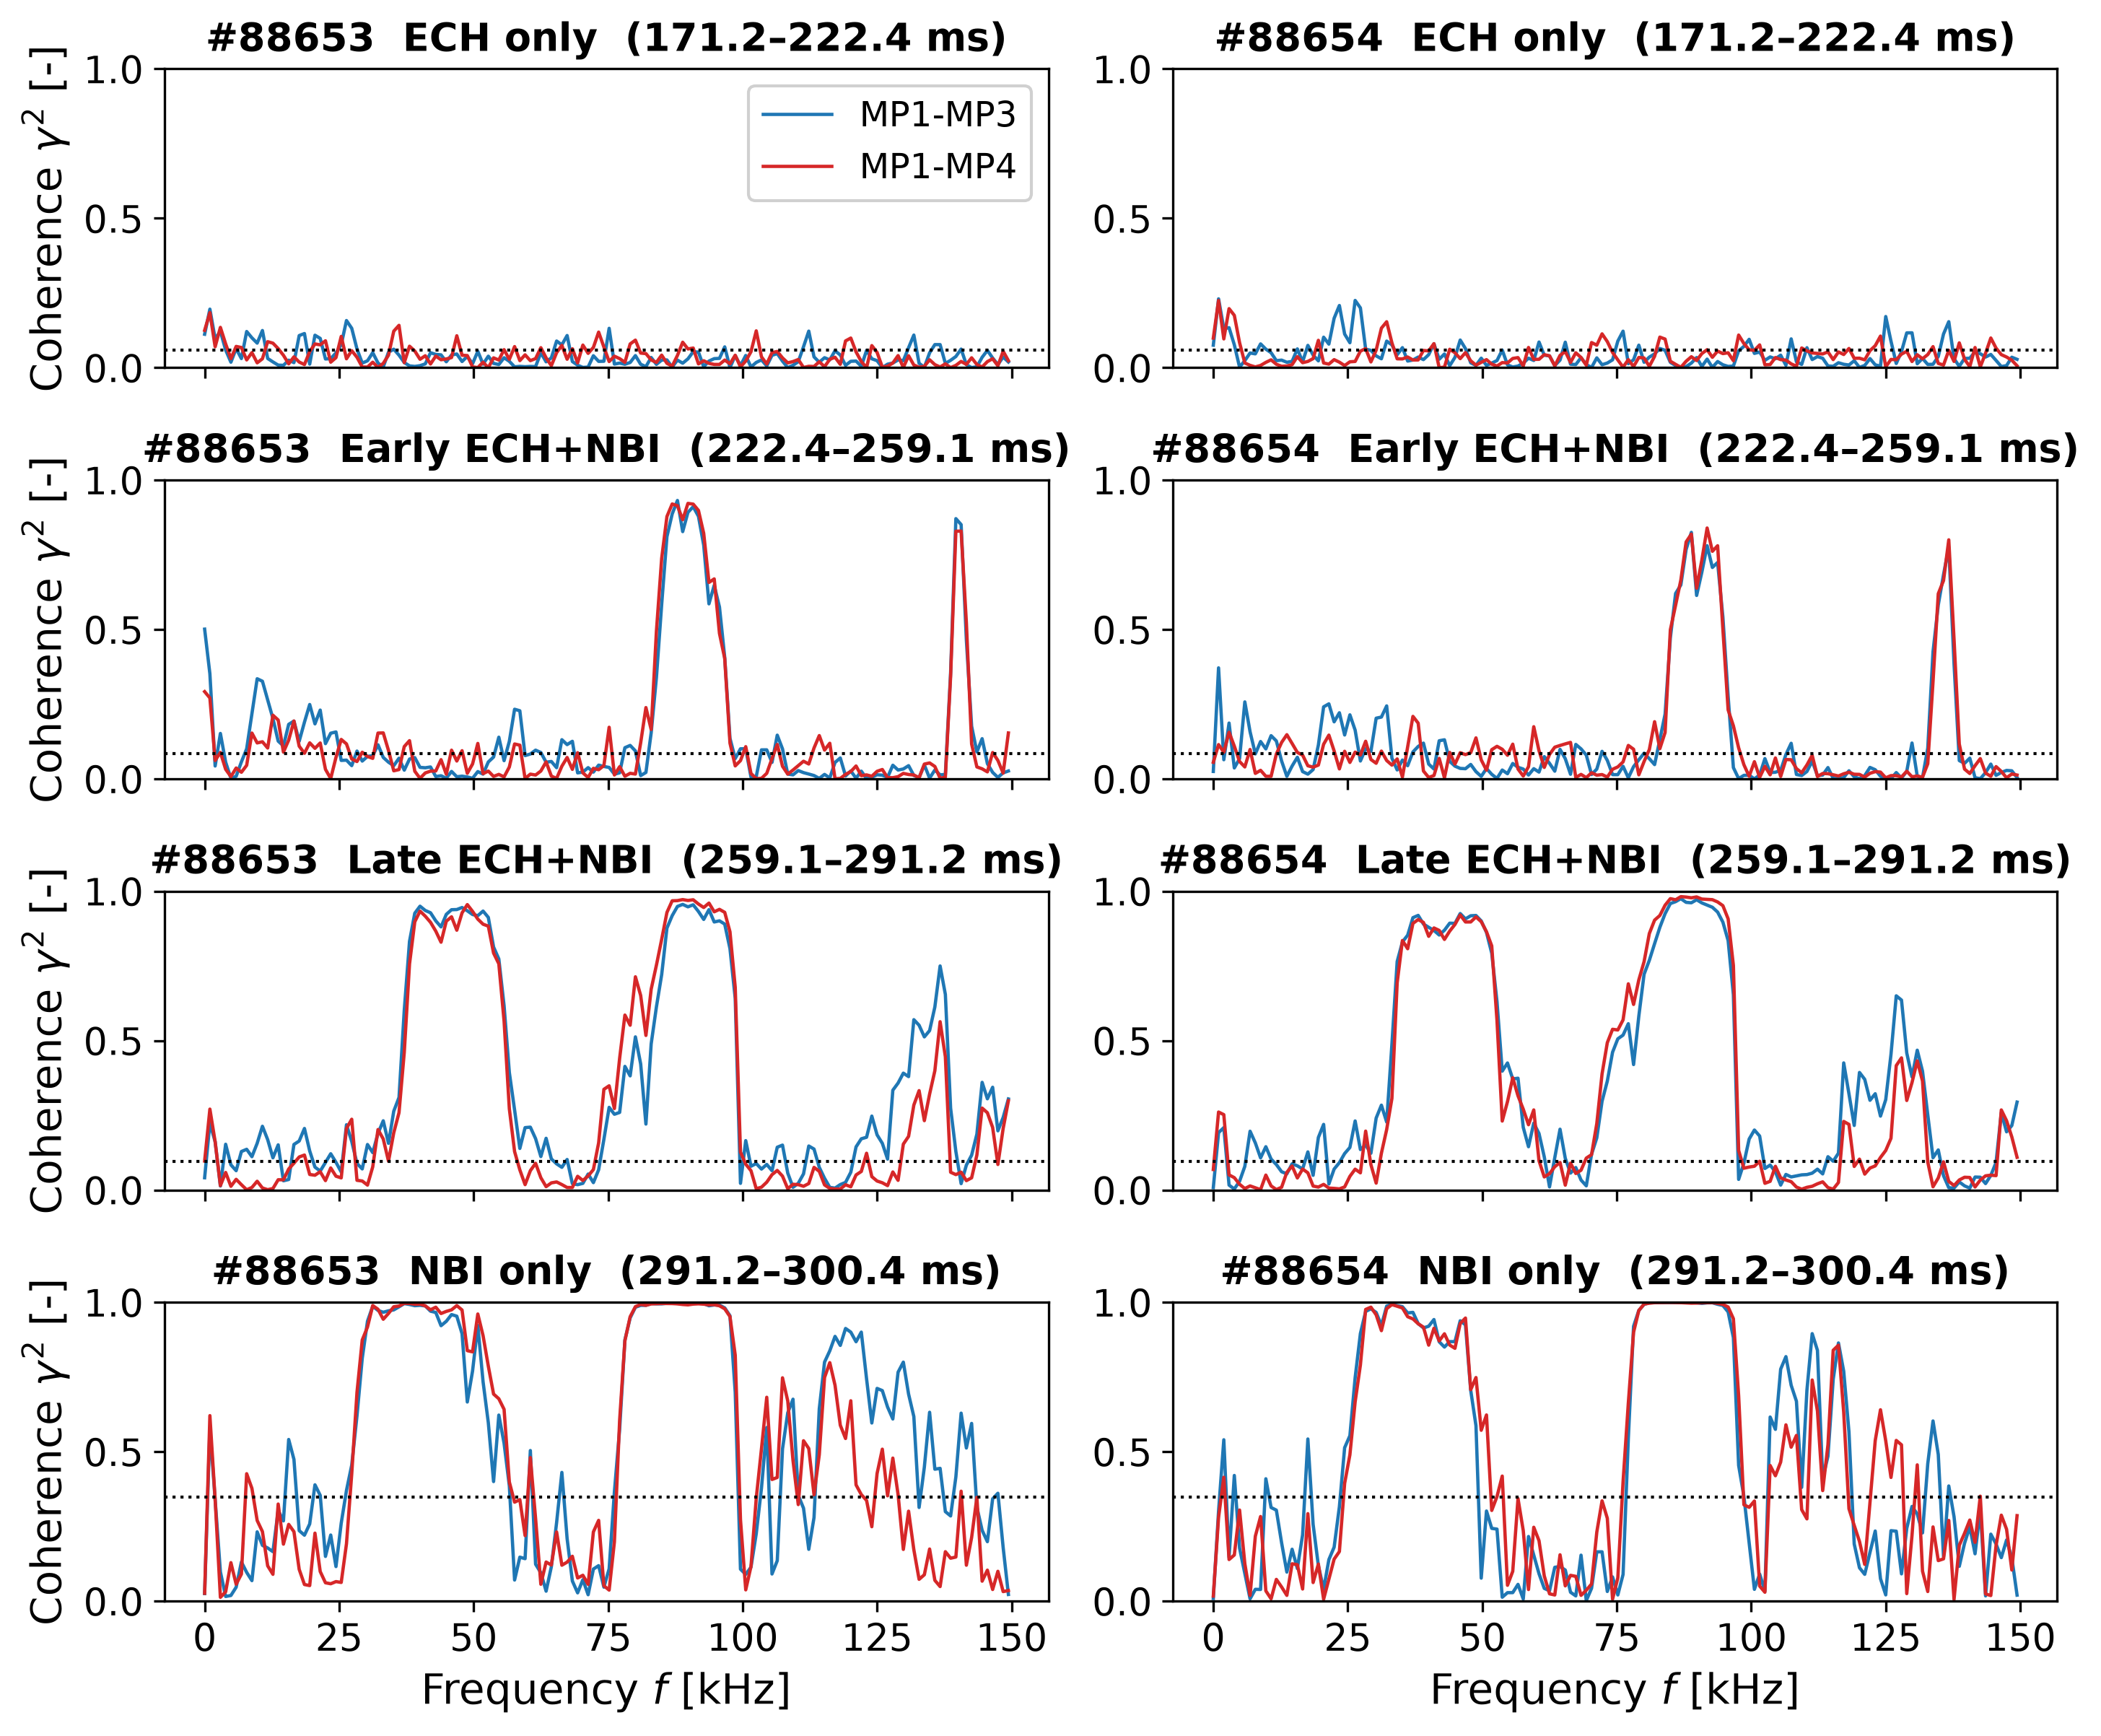
\includegraphics[width=0.88\textwidth]{Images/obj1_mode_identification/fig_coherence_spectra_both_shots.png}
  \caption[Probe coherence by heating phase]{Magnitude-squared coherence ($\gamma^2$) for MP1--MP3 and MP1--MP4 across heating phases in shots \#88653 (left) and \#88654 (right).}
  \label{fig:coherence_spectra}
\end{figure}
Table~\ref{tab:mode_structure} summarized the spatial mode structure across fixed heating windows and post-transition slices. In the primary band ($89.8~\mathrm{kHz}$ in $\mathrm{ECH}+\mathrm{NBI}$; $85.9~\mathrm{kHz}$ in $\mathrm{NBI}$-only), $m = +3$ achieved \emph{supported} status in both phases ($r_{\mathrm{circ}} = 0.882, 0.902$; errors $26.7^\circ, 22.2^\circ$) with $n \equiv -1 \pmod 4$ ($\mathrm{RMSE} = 5.2^\circ, 6.7^\circ$). In the brief post-transition $87~\mathrm{kHz}$ slices, $m = +3$ remained \emph{supported} in \#88654 ($292.0\text{--}293.0~\mathrm{ms}$, $12$ segments, $r_{\mathrm{circ}} = 0.951$, error $15.8^\circ$). In \#88653, however, the shorter $400$-sample slice ($291.4\text{--}291.8~\mathrm{ms}$, $3$ segments) became \emph{unresolved} ($m = +1$, $r_{\mathrm{circ}} = 0.608$, error $65.0^\circ$). Conversely, the secondary band ($48.8~\mathrm{kHz}$ in $\mathrm{ECH}+\mathrm{NBI}$; $41.0~\mathrm{kHz}$ in $\mathrm{NBI}$-only for \#88653) was resolved across both phases by a coexisting two-mode fit $(m_1 = +1, m_2 = +12)$. Both windows achieved \emph{supported} status ($r_{\mathrm{circ}} = 0.832, 0.854$; errors $24.9^\circ, 25.7^\circ$, spanning $11/14$ coils within $|\Delta\phi| \le 45^\circ$), with $n \equiv -1 \pmod 4$ ($\mathrm{RMSE} = 22.7^\circ, 19.3^\circ$). Single-harmonic fits ($m = +2$) failed with $81.1^\circ\text{--}100.9^\circ$ errors and $r_{\mathrm{circ}} = 0.58\text{--}0.63$. These results confirmed a global $m_1 = +1$ mode paired with a steep $m_2 = +12$ branch consistent with helical sideband coupling~\cite{Yamamoto_2020,Varela2024,Adulsiriswad_2024}. While $m_1 = +1$ was cleanly resolved, the $m_2 = +12$ branch approached the spatial Nyquist limit of the 14 irregular coils and could reflect either sideband coupling or spatial aliasing. Multi-phase coherence spectra (Figure~\ref{fig:coherence_spectra}, computed from $1024$-sample Hann segments with $50~\%$ overlap alongside the dotted optimistic $95~\%$ threshold assuming independent segments) confirmed reproducible dual-band excitation across both shots. During ECH-only ($171.2\text{--}222.4~\mathrm{ms}$), $\gamma^2$ stayed near noise; in early $\mathrm{ECH}+\mathrm{NBI}$ ($222.4\text{--}259.1~\mathrm{ms}$), it peaked above $0.8$ near $88$ and $140~\mathrm{kHz}$, before forming $\gamma^2 > 0.9$ plateaus ($35\text{--}55$ and $80\text{--}100~\mathrm{kHz}$) across late heating. Requiring NBI to destabilize both bands and their survival past ECH termination aligned with fast-ion-driven shear-Alfv\'en and EPM branches in Heliotron~J~\cite{Yamamoto_2020,Varela2015,Varela2024}.

\subsubsection{Radial Fluctuation Localization and Multi-Coil Magnetic Coupling}
\label{subsubsec:obj1_radial}

\begin{figure}[H]
  \centering
  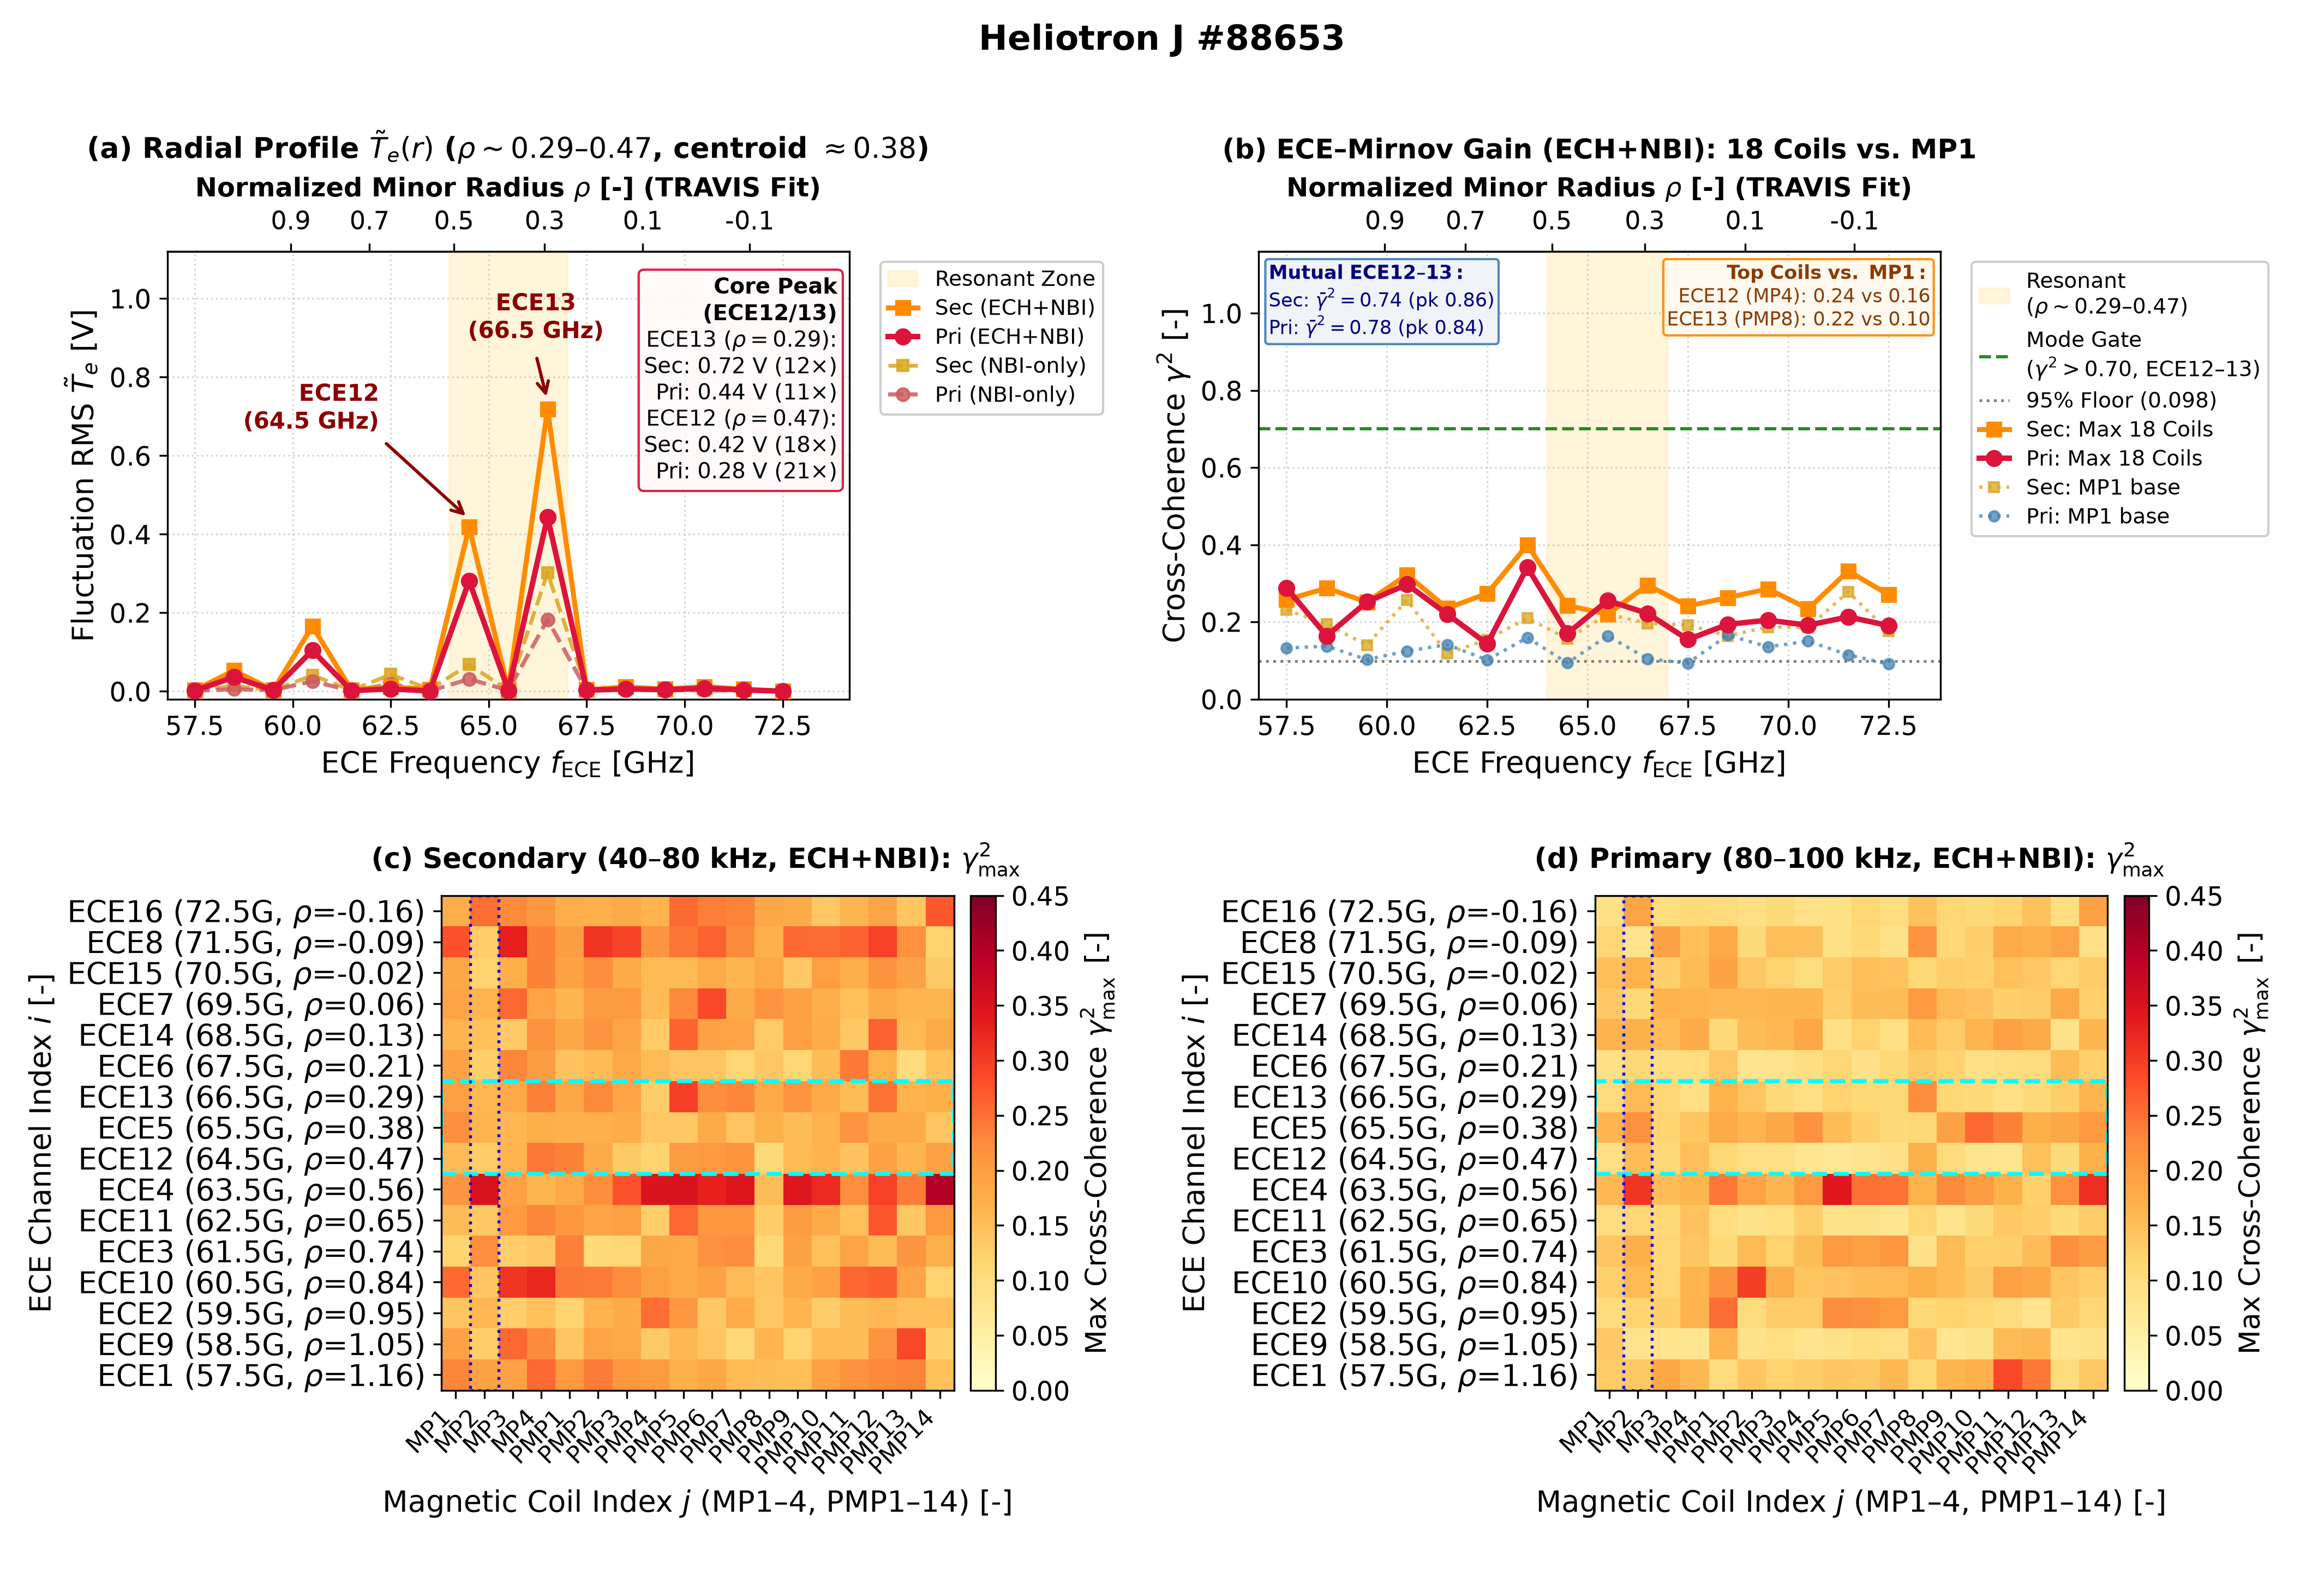
\includegraphics[width=\textwidth]{Images/obj1_mode_identification/mhd_ece_all_probes_radial_localization_88653.png}
  \caption[ECE radial localization and multi-coil magnetic coherence]{Radial localization and ECE--Mirnov coherence ($\mathrm{ECH}+\mathrm{NBI}$) in \#88653: (a)~ECE profile and (b--d)~$16\text{ ECE} \times 18\text{ Coil}$ coupling.}
  \label{fig:obj1_ece_radial}
\end{figure}

Figure~\ref{fig:obj1_ece_radial} presented radial localization and electromagnetic coupling across all 16 ECE channels ($57.5\text{--}72.5~\mathrm{GHz}$) and all 18 Mirnov coils (MP1--MP4, including non-coplanar MP2, and PMP1--PMP14). In Figure~\ref{fig:obj1_ece_radial}(a), the fluctuation RMS profile $\tilde{T}_e$ for both secondary ($40\text{--}80~\mathrm{kHz}$) and primary ($80\text{--}100~\mathrm{kHz}$) bands peaked sharply at \texttt{ECE12FAST} ($64.5~\mathrm{GHz}$, $\rho = 0.465$, $r \approx 7.91~\mathrm{cm}$) and \texttt{ECE13FAST} ($66.5~\mathrm{GHz}$, $\rho = 0.294$, $r \approx 4.99~\mathrm{cm}$). Together with the ${\approx}1~\mathrm{GHz}$ IF bandwidth and \textsc{TRAVIS} calibration (Eq.~(\ref{eqn:ece_travis_fit}), $\Delta \rho \approx 0.08\text{--}0.09$), these channels defined the core-to-mid gradient interval $\rho \approx 0.29\text{--}0.47$ ($\rho_{\mathrm{centroid}} \approx 0.380$, $r \approx 6.45~\mathrm{cm}$, within $\rho \in [0.25, 0.51]$).

During $\mathrm{ECH}+\mathrm{NBI}$ ($259.1\text{--}291.3~\mathrm{ms}$), secondary-band bandpass RMS reached $0.719~\mathrm{V}$ ($12.0\times$ pre-plasma noise) on \texttt{ECE13FAST} and $0.419~\mathrm{V}$ ($18.0\times$) on \texttt{ECE12FAST}; primary-band amplitudes reached $0.444~\mathrm{V}$ ($11.4\times$) and $0.281~\mathrm{V}$ ($21.1\times$), respectively. In the post-transition $\mathrm{NBI}$-only phase ($291.3\text{--}300.0~\mathrm{ms}$), \texttt{ECE13FAST} retained $0.302~\mathrm{V}$ ($5.0\times$) and $0.183~\mathrm{V}$ ($4.7\times$) across the secondary and primary bands. Adjacent \texttt{ECE12FAST}--\texttt{ECE13FAST} mutual coherence during $\mathrm{ECH}+\mathrm{NBI}$ reached $\gamma^2_{\mathrm{mean}} = 0.74$ ($\gamma^2_{\max} = 0.86$) in $40\text{--}80~\mathrm{kHz}$ and $0.78$ ($0.84$) in $80\text{--}100~\mathrm{kHz}$; given shared Bank~B baseline coupling ($\gamma^2_{\mathrm{mean}} \approx 0.74\text{--}0.83$ at $150\text{--}170~\mathrm{ms}$), mode confirmation rested jointly on the core RMS surge, selective $\mathrm{NBI}$-only peaks ($0.95\text{--}0.98$), and Mirnov coherence.

\paragraph*{Radial Phase Delay and Direction of Wave and Energy Propagation (\texttt{ECE13FAST} \texorpdfstring{$\leftrightarrow$}{<->} \texttt{ECE12FAST}).}
Cross-spectral density (CSD) phases $\Delta\phi_{13\to 12}(f) = \arg\langle \mathcal{H}(y_{13})\mathcal{H}^*(y_{12})\rangle$ and correlation lags $\Delta\tau_{13\to 12} = t_{12} - t_{13}$ resolved radial propagation between \texttt{ECE13FAST} ($\rho = 0.294$) and \texttt{ECE12FAST} ($\rho = 0.465$). This interval spanned $\Delta\rho = 0.171$ ($\Delta r \approx 2.92~\mathrm{cm}$) across carrier, envelope, and sawtooth bands. By convention, $\Delta\phi_{13\to 12} > 0$ ($\Delta\tau > 0$, channel $13$ leading channel $12$) indicated outward propagation ($13 \to 12$), consistent with outward cross-field heat transport and stored-energy degradation. Conversely, $\Delta\phi_{13\to 12} < 0$ ($\Delta\tau < 0$) denoted inward phase progression ($12 \to 13$).

This comparison (Figure~\ref{fig:ece_phase_delay}) revealed a clear physical dichotomy between the fast carrier phase velocity and wavepacket group transport. In the high-frequency carrier band during $\mathrm{ECH}+\mathrm{NBI}$, continuous phase delays were negative rather than quantized at $1~\mu\mathrm{s}$ steps. Secondary fluctuations ($40\text{--}80~\mathrm{kHz}$) gave $\Delta\phi_{13\to 12} = -10.8^\circ$ ($\Delta\tau = -0.51~\mu\mathrm{s}$, $r = +0.841$), while primary fluctuations ($80\text{--}100~\mathrm{kHz}$) gave $-12.7^\circ$ ($\Delta\tau = -0.39~\mu\mathrm{s}$, $r = +0.863$). These corresponded to an apparent inward phase velocity $v_{\mathrm{ph},r} \approx -57\text{ to }-75~\mathrm{km/s}$ (replicated in \#88654 at $-11.1^\circ$ and $-12.9^\circ$). Beyond wave propagation, steady negative phase offsets between adjacent ECE channels (both \texttt{ECE12FAST} and \texttt{ECE13FAST} belonged to local oscillator (LO) Bank~B) could also reflect an eigenmode radial phase tilt or minor sub-microsecond inter-channel IF or digitizer skew. Conversely, Hilbert envelopes $|\mathcal{H}|$ propagated outward: the primary envelope yielded $\Delta\tau_{\mathrm{env}} = +0.82~\mu\mathrm{s}$ ($r = 0.768$) in $\mathrm{ECH}+\mathrm{NBI}$, $+1.34~\mu\mathrm{s}$ in the sawtooth window, and $+1.37~\mu\mathrm{s}$ in $\mathrm{NBI}$-only ($v_{\mathrm{g},r} \approx +22\text{ to }+36~\mathrm{km/s}$). Mesoscopic sawtooth modulation ($277.0\text{--}294.0~\mathrm{ms}$) propagated outward at $+8.0~\mu\mathrm{s}$ (primary, $+4.0^\circ$, $r = +0.897$) and $+40.0~\mu\mathrm{s}$ (secondary, $+16.7^\circ$, $r = +0.671$). Similarly, the post-ECH thermal decay pulse ($0.35\text{--}2.2~\mathrm{kHz}$) moved outward at $+46.6~\mu\mathrm{s}$ ($+15.9^\circ$, $r = +0.782$ in \#88653; $+55.2~\mu\mathrm{s}$ in \#88654). Physically, the carrier phase reflected an inward-tilted radial eigenmode structure~\cite{zang2019observation,Zhong2024,luo2020measurement}, while wavepackets and thermal pulses transported energy radially outward across $\rho = 0.294\text{--}0.465$, consistent with core EPM/BAE observations~\cite{Weir2019,Kin2025}.

\begin{figure}[H]
  \centering
  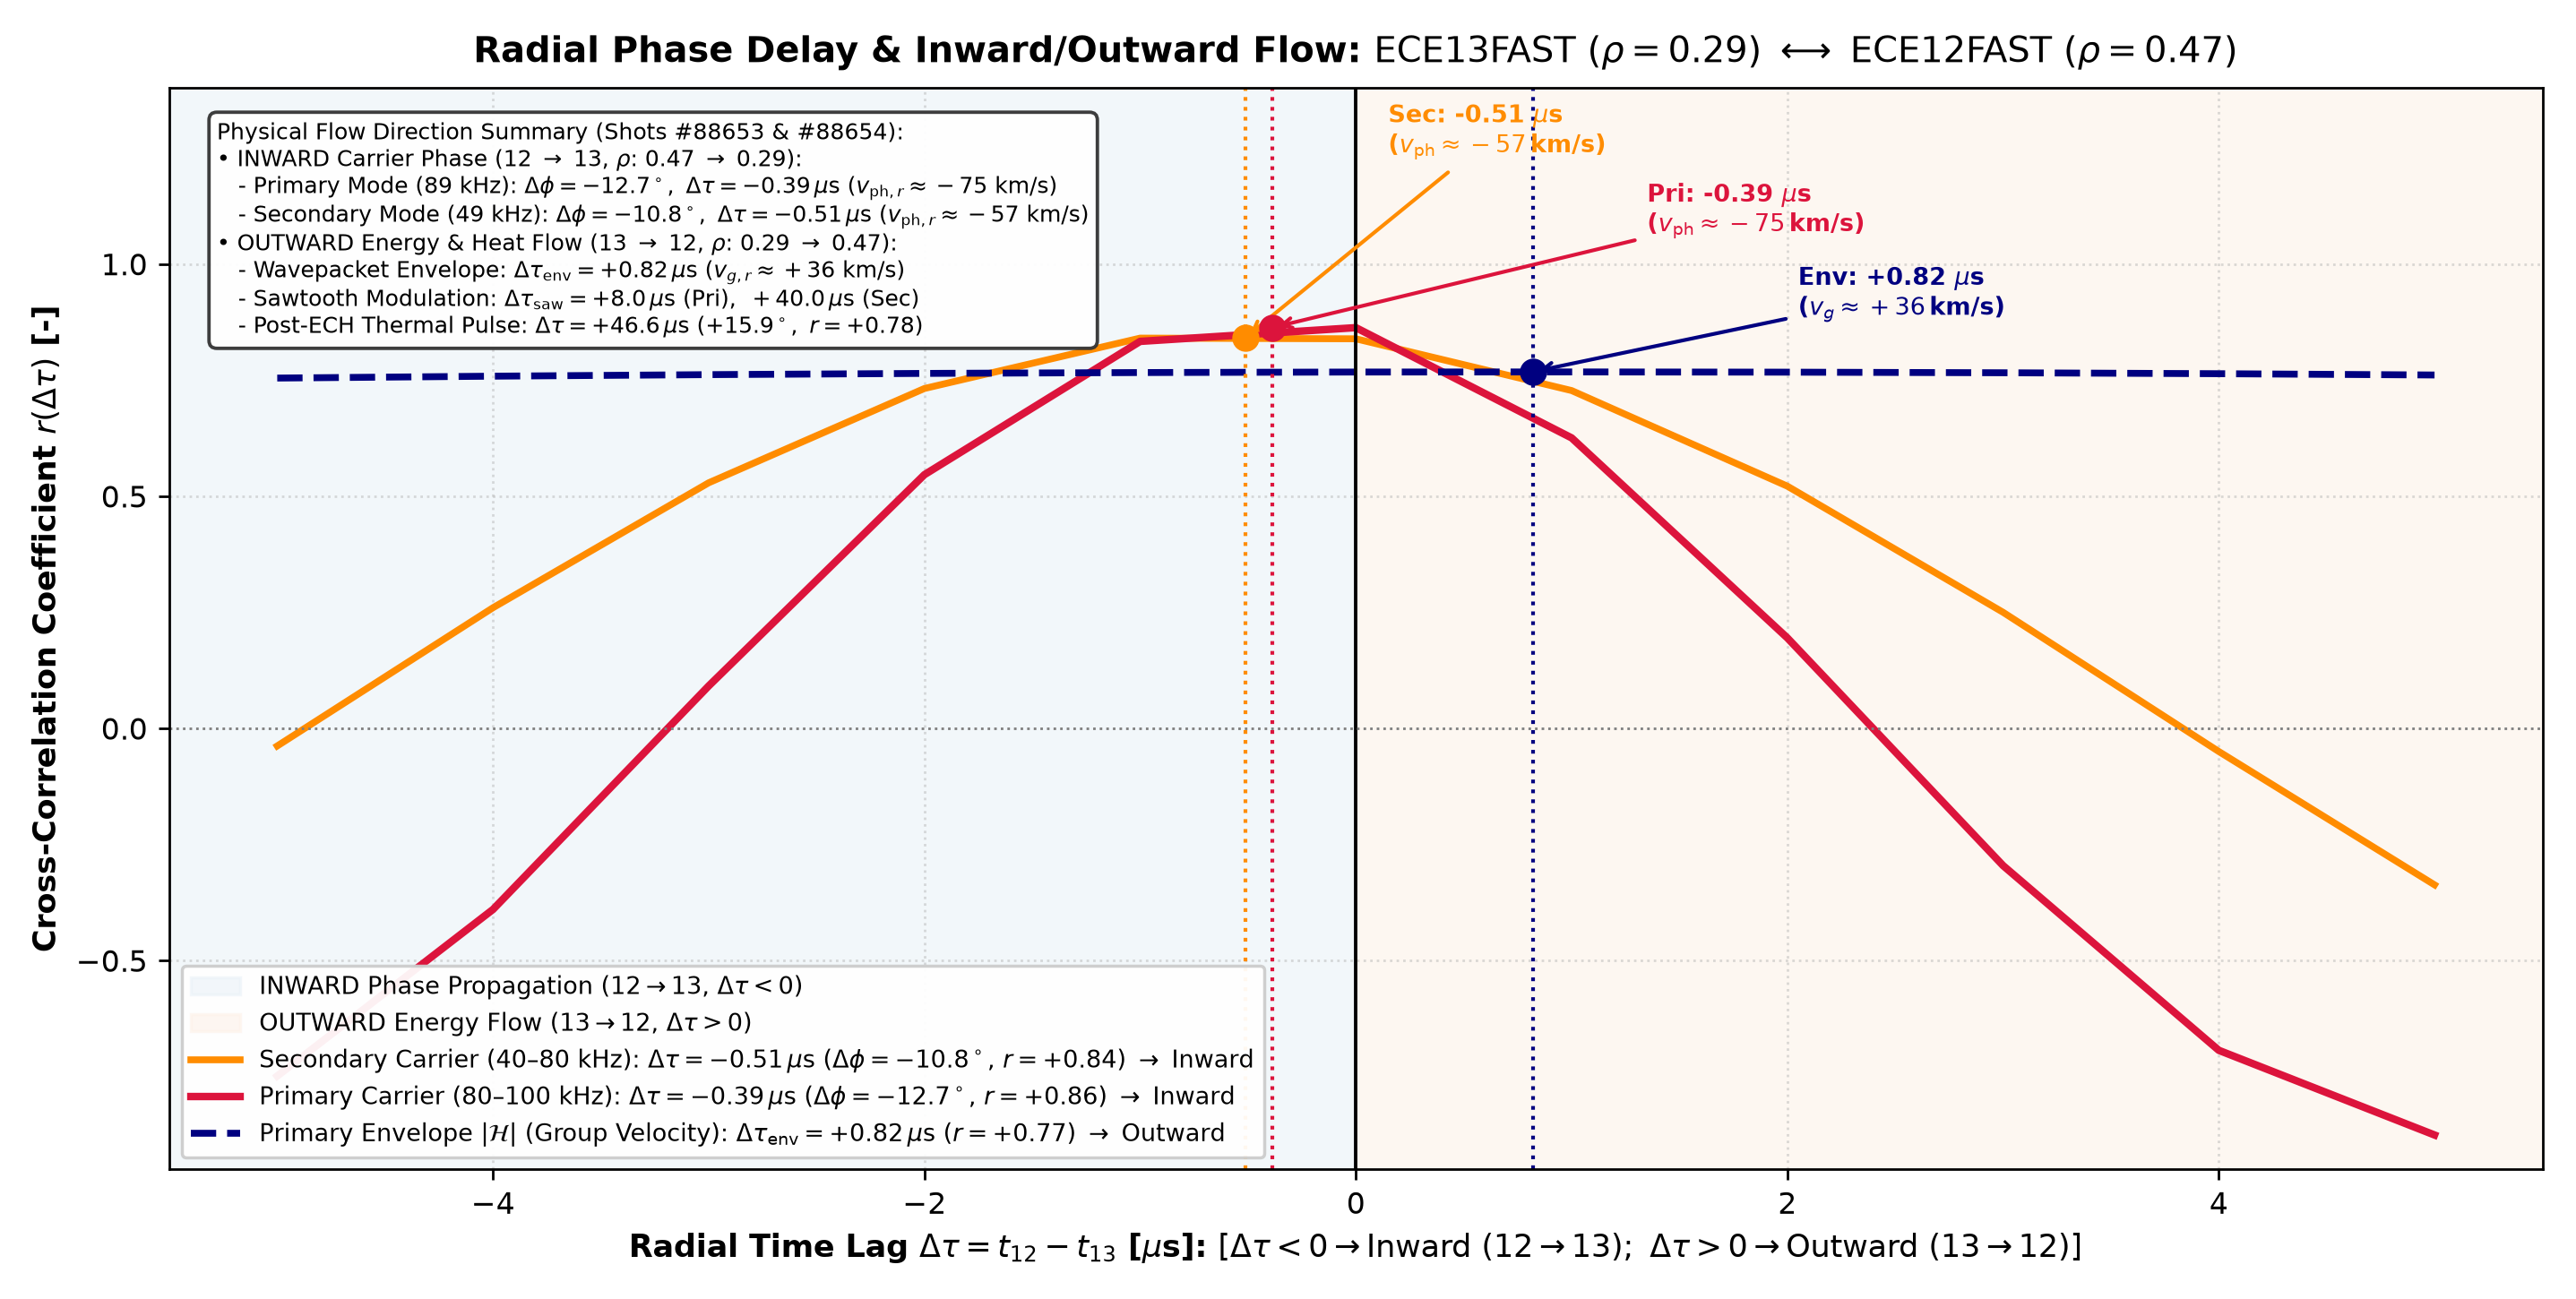
\includegraphics[width=0.95\textwidth]{Images/obj1_mode_identification/mhd_ece12_13_phase_delay_flow_88653.png}
  \caption[Radial phase delay and wavepacket group propagation between ECE13FAST and ECE12FAST]{Lagged cross-correlation $r(\Delta\tau)$ between \texttt{ECE13FAST} ($\rho = 0.294$) and \texttt{ECE12FAST} ($\rho = 0.465$) during $\mathrm{ECH}+\mathrm{NBI}$ in shot \#88653, comparing inward carrier phase delays ($\Delta\tau < 0$) against outward wavepacket envelope transport ($\Delta\tau_{\mathrm{env}} = +0.82~\mu\mathrm{s}$).}
  \label{fig:ece_phase_delay}
\end{figure}

Scanning $16\text{ ECE} \times 18\text{ Coil}$ ECE--Mirnov coherence during $\mathrm{ECH}+\mathrm{NBI}$ (Figure~\ref{fig:obj1_ece_radial}(b--d)) resolved a single-probe limitation and explained why cross-diagnostic $\gamma^2_{\max}$ stayed below internal ECE--ECE levels. Core ECE ($\tilde{T}_e$) versus vessel-wall Mirnov ($\mathrm{d}\tilde{B}_\theta/\mathrm{d}t$) separation, uncorrelated $70~\mathrm{GHz}$ ECH broadband power, and $17.4~\%$ \texttt{ECE13FAST} rail clipping diluted $\gamma^2$ on MP1 ($0.093\text{--}0.104$ primary; $0.156\text{--}0.196$ secondary), yet multi-coil scanning cleared the $95~\%$ floor ($\gamma^2_{95\%} = 0.049, 0.098$ for $N_{\mathrm{fft}}=1024, 2048$). In $40\text{--}80~\mathrm{kHz}$, coherence reached $\gamma^2 = 0.322$ (\texttt{ECE10FAST} / MP4), $0.295$ (\texttt{ECE13FAST} / PMP5), and $0.242$ (\texttt{ECE12FAST} / MP4), with $|r_{\mathrm{env}}| = 0.287$ (\texttt{ECE12FAST} / MP4). In $80\text{--}100~\mathrm{kHz}$, coherence reached $0.297$ (\texttt{ECE10FAST} / PMP2) and $0.222$ (\texttt{ECE13FAST} / PMP8), with $|r_{\mathrm{car}}| = 0.122$ (\texttt{ECE5FAST} / MP2) and $|r_{\mathrm{env}}| = 0.205$ (\texttt{ECE9FAST} / PMP12) and $0.199$ (\texttt{ECE12FAST} / PMP12).

Switching off the $70~\mathrm{GHz}$ ECH source in the $\mathrm{NBI}$-only phase ($291.3\text{--}300.0~\mathrm{ms}$) eliminated RF pickup and substantially strengthened ECE--Mirnov coupling across internal and outer-gradient channels. Within the secondary band, $|r_{\mathrm{car}}|$ reached $0.404$ (\texttt{ECE12FAST} / MP4) and $0.400$ (\texttt{ECE13FAST} / MP4), while $|r_{\mathrm{env}}|$ reached $0.553$ (\texttt{ECE13FAST} / MP4) and coherence peaked at $\gamma^2 = 0.799$ (\texttt{ECE13FAST} / PMP13 at $44.9~\mathrm{kHz}$) and $0.661$ (\texttt{ECE12FAST} / PMP2). For the primary mode, carrier correlation reached $|r_{\mathrm{car}}| = 0.411$ (\texttt{ECE11FAST} / PMP14) and $0.284$ (\texttt{ECE13FAST} / MP3), and envelope correlation reached $|r_{\mathrm{env}}| = 0.586$ (\texttt{ECE11FAST} / MP2) and $0.518$ (\texttt{ECE13FAST} / MP3). At the $86.0~\mathrm{kHz}$ peak, off-midplane coil MP2 ranked highest ($\gamma^2 = 0.360$ on \texttt{ECE11FAST} / MP2, $\rho = 0.65$; $0.359$ on \texttt{ECE10FAST} / MP2, $\rho = 0.84$), while band-maximum coherence reached $\gamma^2 = 0.670$ (\texttt{ECE13FAST} / PMP2). Although part of the broadband coherence across core-to-outer-gradient ECE channels (\texttt{ECE13FAST} to \texttt{ECE10FAST}, $\rho = 0.29\text{--}0.84$) during $291.3\text{--}293.5~\mathrm{ms}$ reflected post-ECH equilibrium relaxation, the step-free steady tail ($294.2\text{--}300.0~\mathrm{ms}$) confirmed persistent mode-specific coherence. Tail coherence exceeded the $95~\%$ floor at $\gamma^2 = 0.350$ on \texttt{ECE13FAST} / PMP11 ($40\text{--}80~\mathrm{kHz}$), alongside $0.301$ on \texttt{ECE14FAST} / PMP13 and $0.275$ on \texttt{ECE15FAST} / MP2 ($80\text{--}100~\mathrm{kHz}$).

\begin{figure}[H]
  \centering
  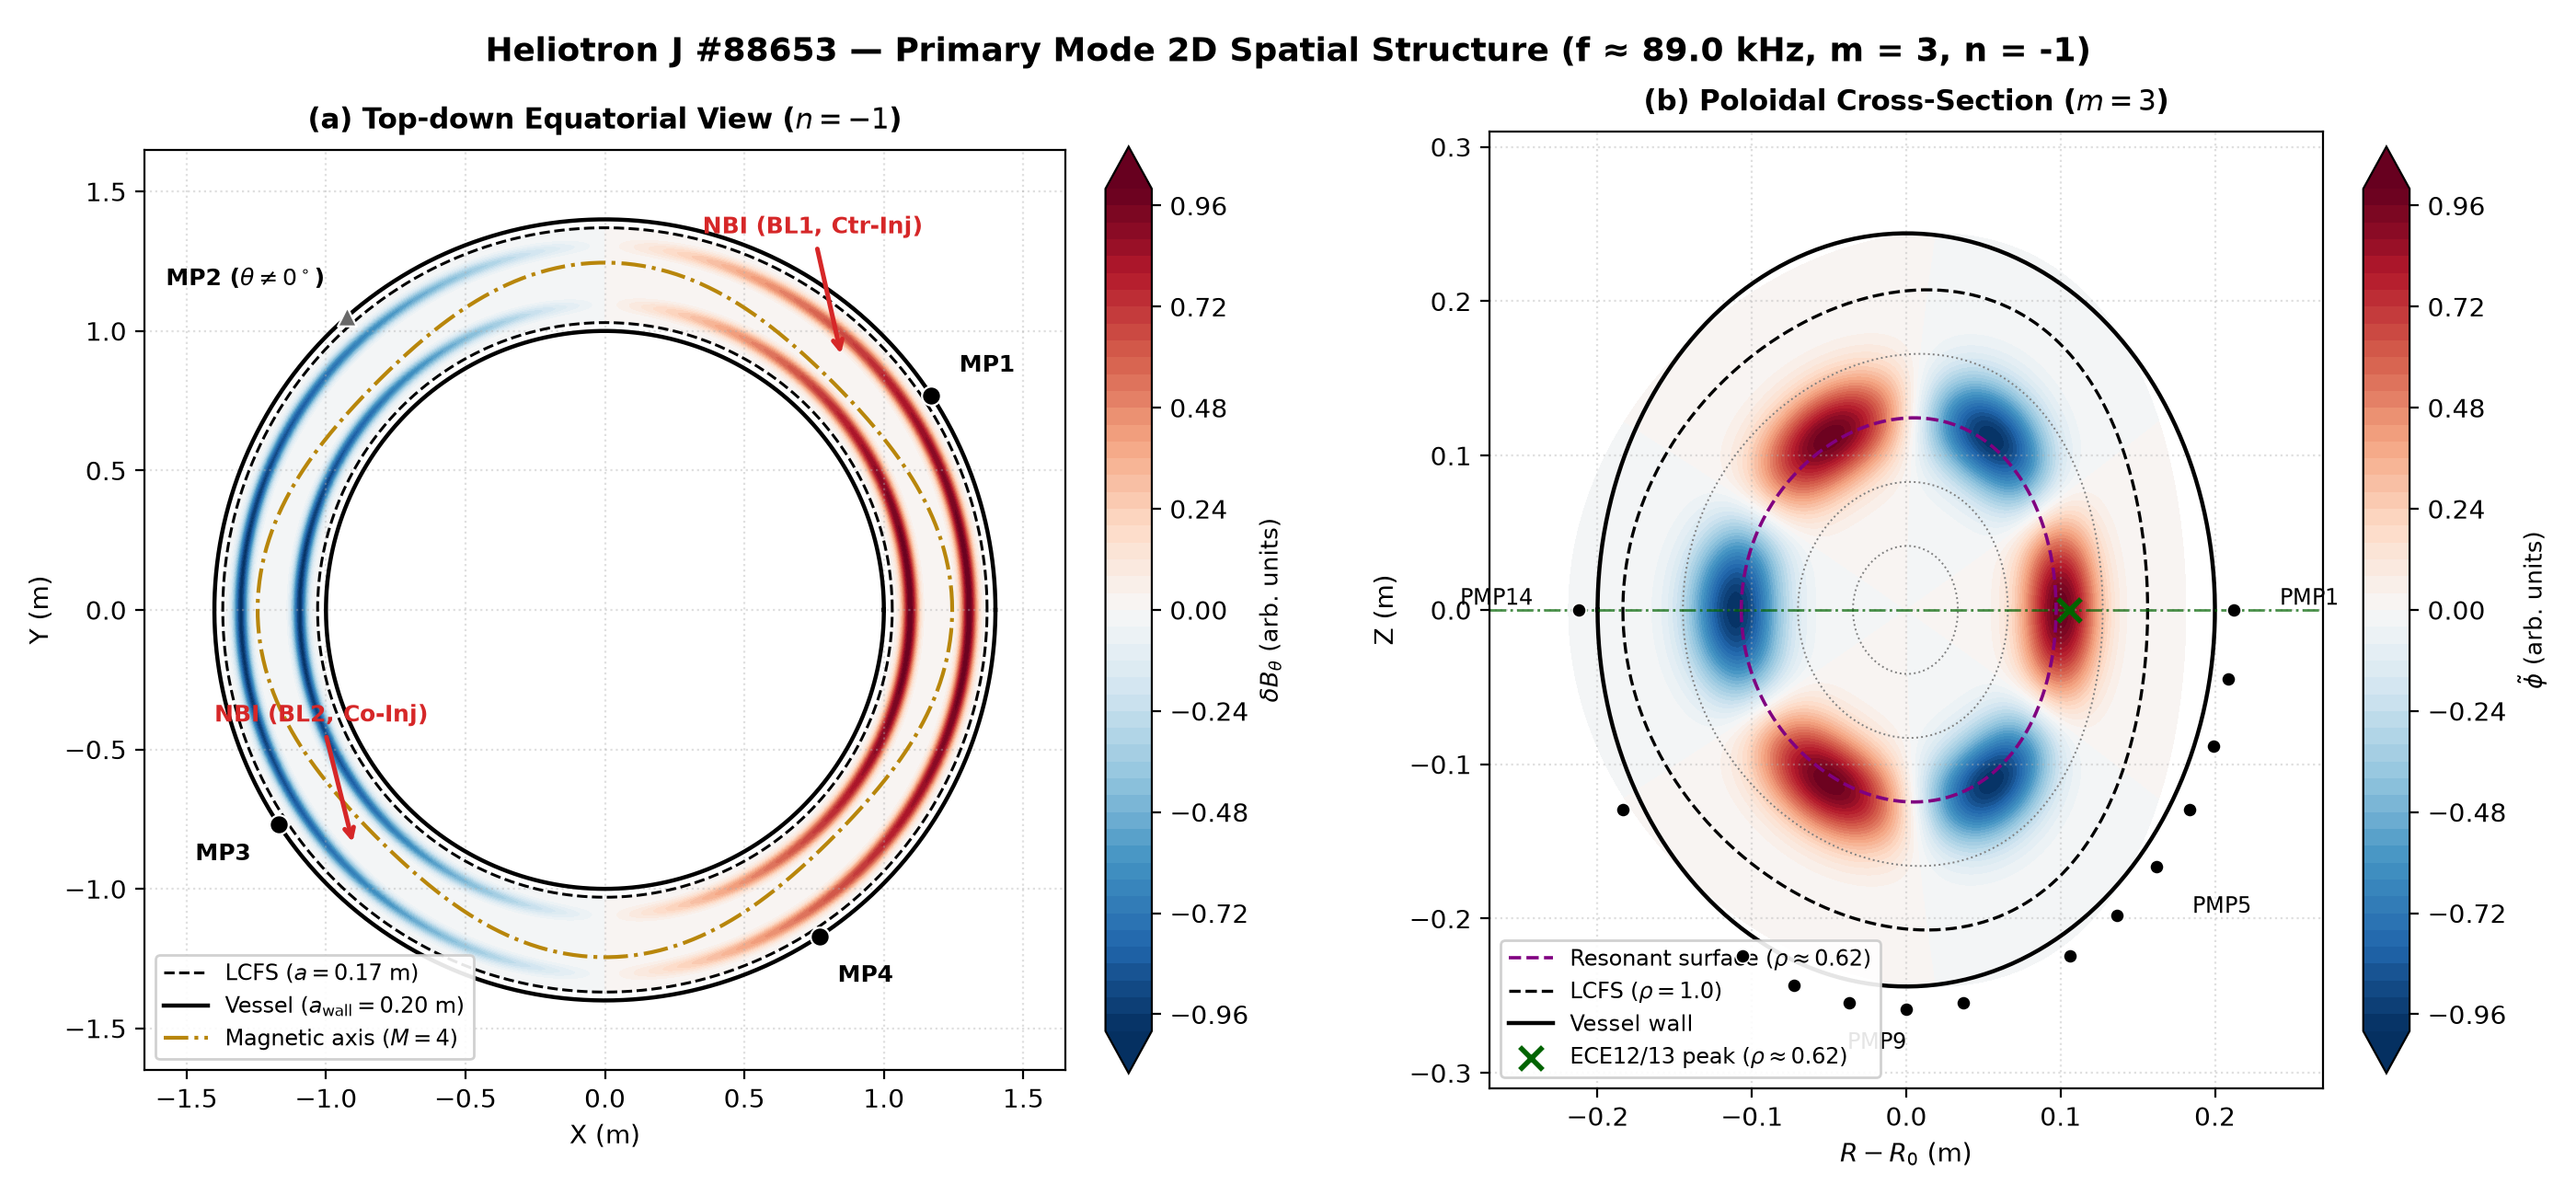
\includegraphics[width=0.98\textwidth]{Images/obj2_dynamics_and_structure/mhd_mode_spatial_map_2d_88653.png}
  \caption[2D schematic representation of the fitted MHD mode structures]{2D schematic of fitted MHD mode structures in shot \#88653: (a)~equatorial view and (b, c)~poloidal cross-sections.}
  \label{fig:obj1_spatial_map_2d}
\end{figure}

Figure~\ref{fig:obj1_spatial_map_2d} synthesized these structural findings into a 2D schematic representation of the fitted mode harmonics (normalized) overlaid on the equilibrium and diagnostic layout within the last closed flux surface (LCFS, $\rho = 1.0$, $a = 0.17~\mathrm{m}$): panel~(a) showed the equatorial plane ($Z = 0$) with $n \equiv -1 \pmod 4$, toroidal probes MP1--MP4, and the ECE sightline, whereas panels~(b, c) displayed poloidal cross-sections over PMP1--PMP14 for the secondary ($m_1 = +1 \wedge m_2 = +12$) and primary ($m = +3$) harmonics across the $\rho \sim 0.29\text{--}0.47$ resonant zone. Combining the poloidal numbers ($m=+3$ primary; coexisting $m_1=+1 \wedge m_2=+12$ secondary), toroidal mode number ($n \equiv -1 \pmod 4$), and radial birth zone localized the instability in the core-to-mid gradient region. This spatial co-localization of the $m/n = 3/-1$ and $(1, 12)/-1$ modes established the shared resonant layer governing energetic-particle drive, rational-surface alignment, and nonlinear wave--wave interactions.

\subsubsection{Dynamic Behavior and Frequency Evolution}
\label{subsubsec:obj1_dynamics}
As shown in Figures~\ref{fig:obj1_spectrogram} and~\ref{fig:coherence_spectra}, both primary ($80\text{--}100~\mathrm{kHz}$) and secondary ($35\text{--}55~\mathrm{kHz}$) modes persisted throughout late $\mathrm{ECH}+\mathrm{NBI}$ ($259.1\text{--}291.3~\mathrm{ms}$). Both bands chirped upward over $259\text{--}275~\mathrm{ms}$ before stabilizing, then survived into post-ECH $\mathrm{NBI}$-only heating ($291.3\text{--}300.4~\mathrm{ms}$, $\gamma^2 > 0.95$) with downward frequency sweeping until NBI shut-off (\emph{supported}, though the brief $9.1~\mathrm{ms}$ window bounded spectral resolution). Comparable upward chirping followed by downward relaxation during fast-ion drive and $T_e$ decay characterized resonant EPM and BAE branches~\cite{Zhong2024,Varela2023,Yamamoto_2020}.

\subsubsection{Response to ECH Switch-Off}
\label{subsubsec:obj1_ech_off}

\begin{table}[H]
\centering
\small
\setlength{\tabcolsep}{4.5pt}
\renewcommand{\arraystretch}{1.15}
\caption[Heating phases and Mirnov spectral summary for shot \#88653]{Heating phases and Mirnov spectral summary for shot \#88653.}
\label{tab:discharge_phases}
\begin{tabular}{lccccrl}
\toprule
Phase & \shortstack{Coherence\\window (ms)} & \shortstack{RMS\\window (ms)} & \shortstack{MP1\\RMS (V)} & \shortstack{Peak\\$\gamma^2$ (-)} & \shortstack{Power /\\threshold (-)} & \shortstack{Discrete\\modes (kHz)} \\
\midrule
Pre-plasma & 150.0--171.2 & 150.0--171.2 & 0.016 & 0.765 & 0.7 & none \\
ECH only & 171.2--222.4 & 171.0--222.0 & 0.040 & 0.158 & 33.8 & none \\
Early ECH+NBI & 222.4--259.1 & 222.0--259.0 & 0.087 & 0.931 & 450.6 & 87.9, 139.6 \\
Late ECH+NBI & 259.1--291.2 & 259.0--291.0 & 0.274 & 0.972 & 7052.3 & 40.0, 88.9 \\
NBI only & 291.2--300.4 & 291.2--300.4 & 0.281 & 0.997 & 9232.6 & \shortstack[l]{37.1, 50.8,\\86.9, 115.2} \\
\shortstack[l]{Post-heating\\decay} & 300.4--350.0 & 300.4--350.0 & 0.054 & 0.990 & 131.4 & \shortstack[l]{31.2, 35.2, 41.0,\\48.8 (+5)} \\
\bottomrule
\end{tabular}
\par\smallskip{\footnotesize Peak $\gamma^2$ computed from MP1--MP3; RMS amplitude evaluated over the specified time intervals. Pre-plasma exhibits no spectral line above the detection threshold, so its $\gamma^2$ value does not represent a coherent mode. Line frequencies correspond to fixed phase windows and may differ by one STFT bin from those in Table~\ref{tab:mode_structure}.}
\end{table}


\begin{figure}[htbp]
  \centering
  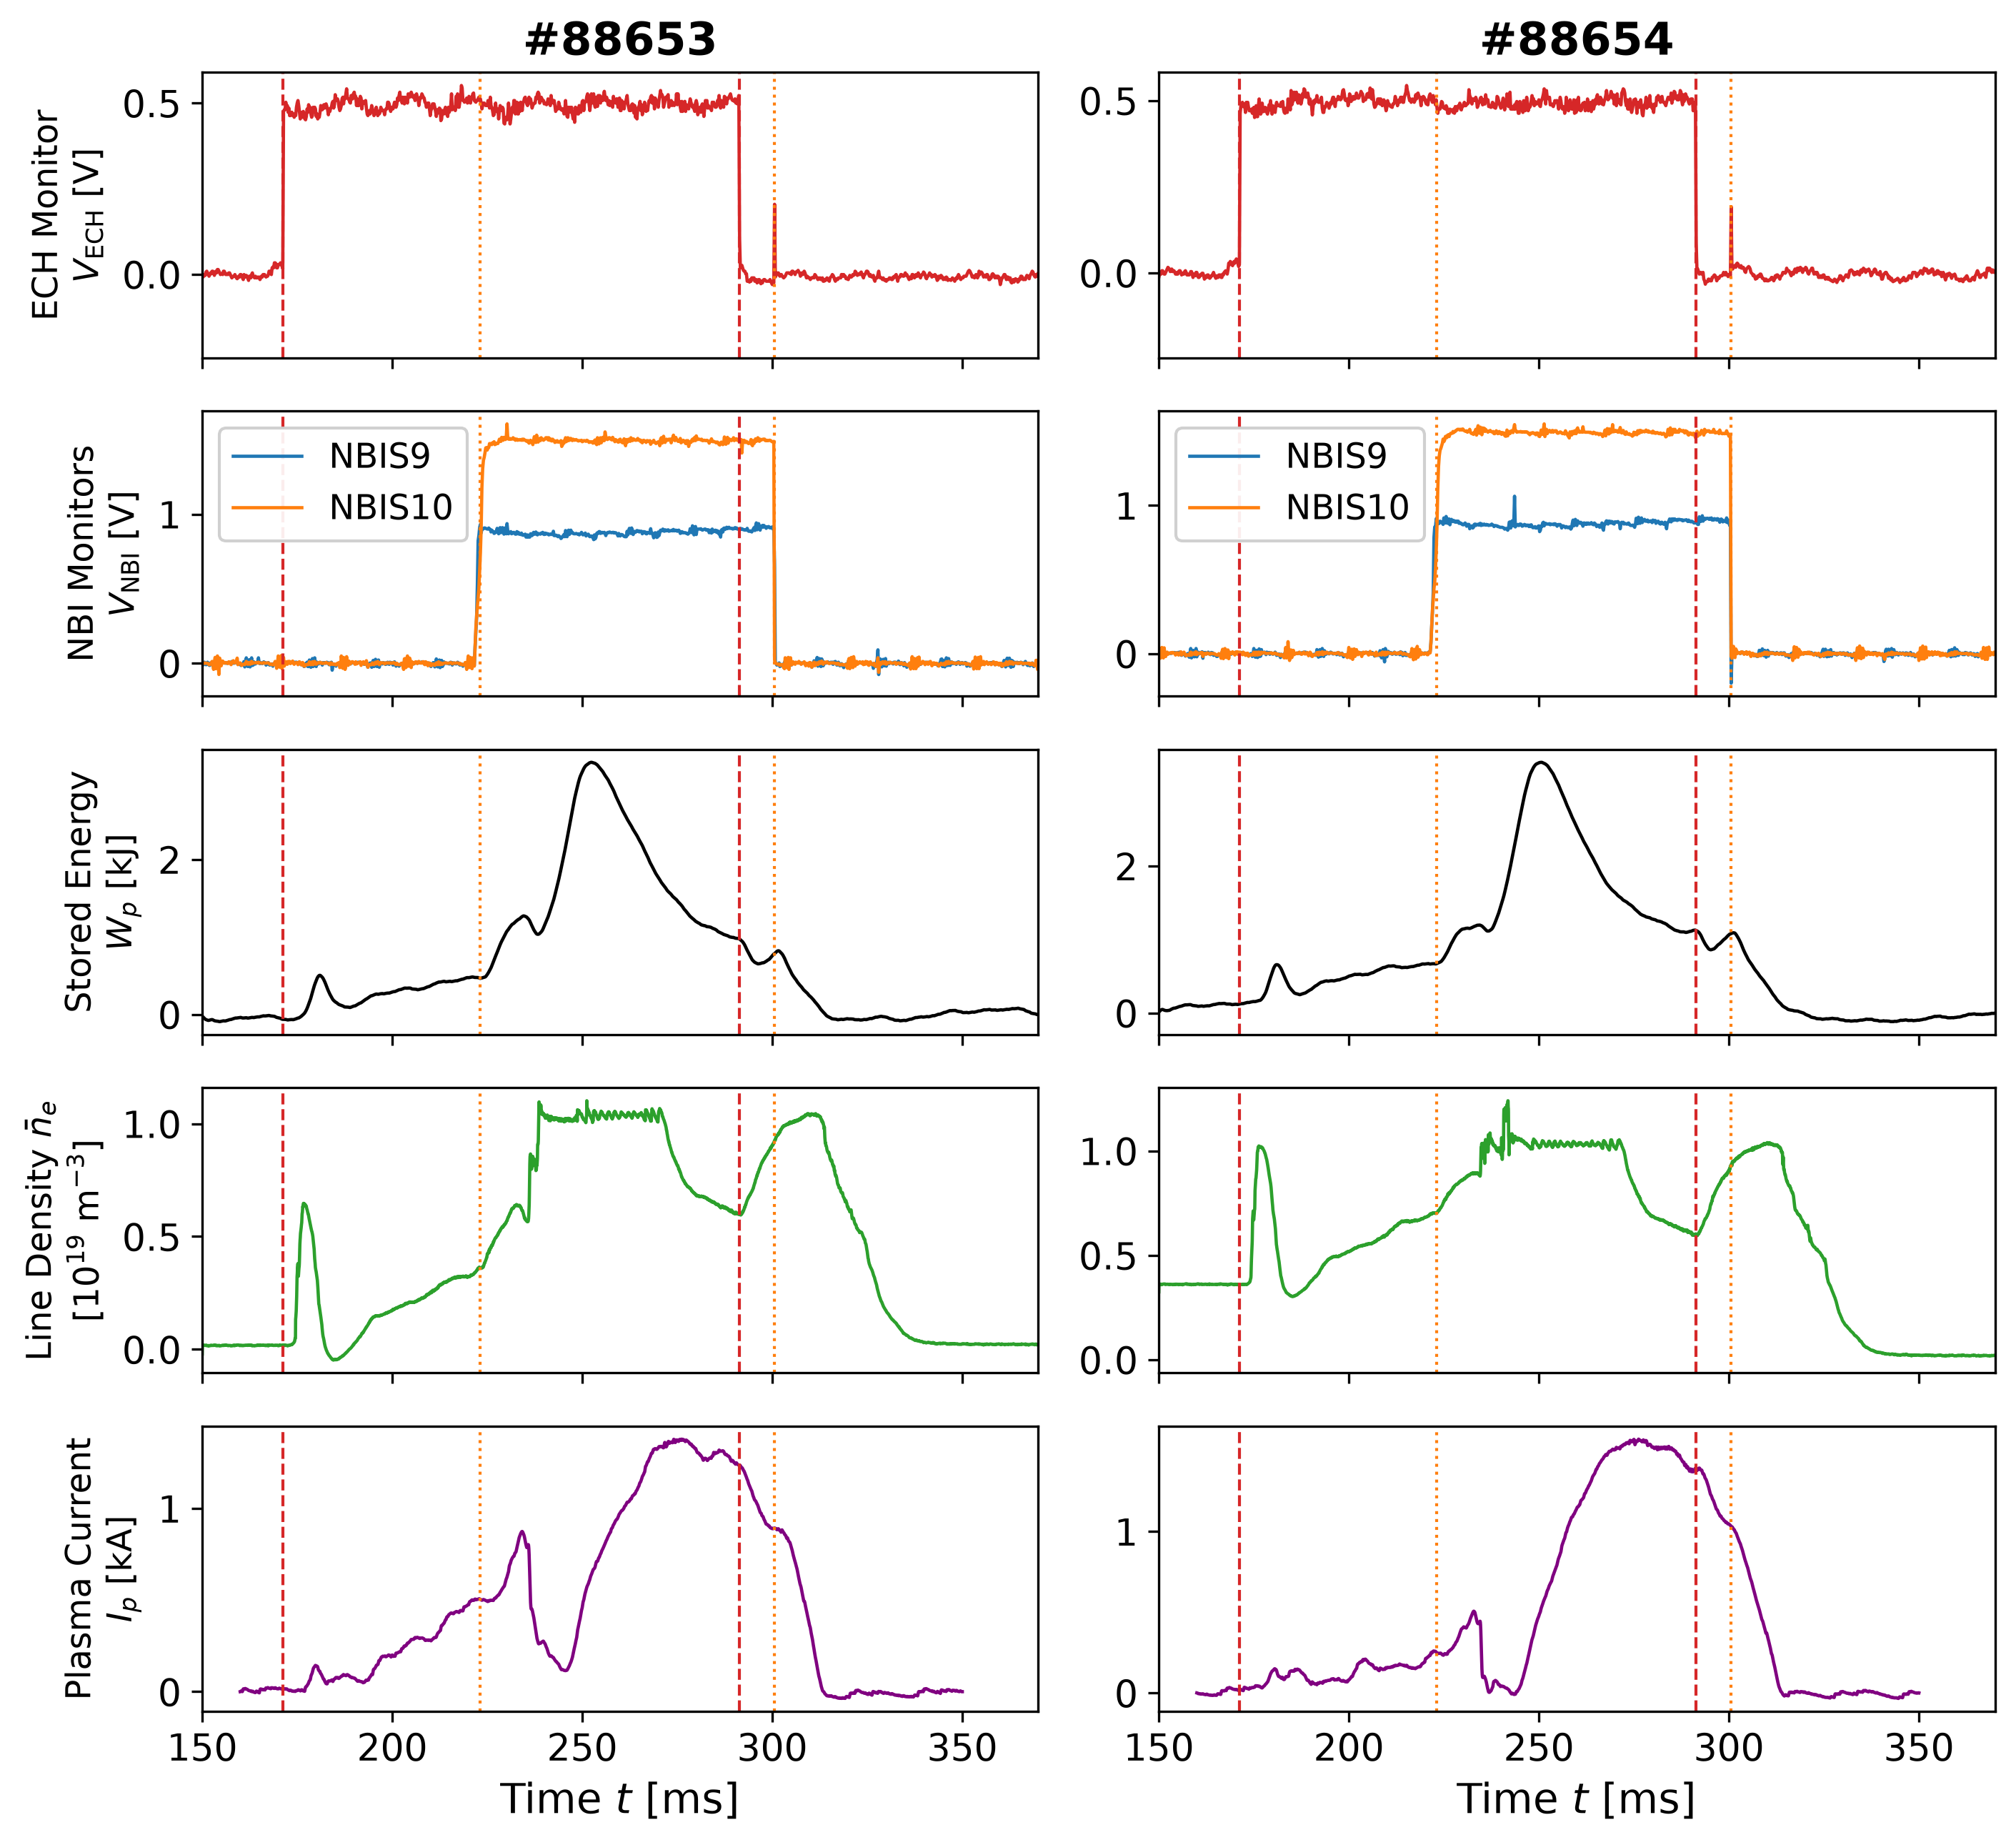
\includegraphics[width=0.80\textwidth]{Images/obj2_dynamics_and_structure/panels/fig_heating_timeline_both_shots.png}
  \caption[Heating signals and \texorpdfstring{$I_p$}{Ip}, both shots]{Heating traces (ECH, NBIS9, NBIS10), $W_p$, $n_e$, and $I_p$ ($150\text{--}370~\mathrm{ms}$) for shots \#88653 and \#88654.}
  \label{fig:heating_timeline}
\end{figure}

\begin{figure}[htbp]
  \centering
  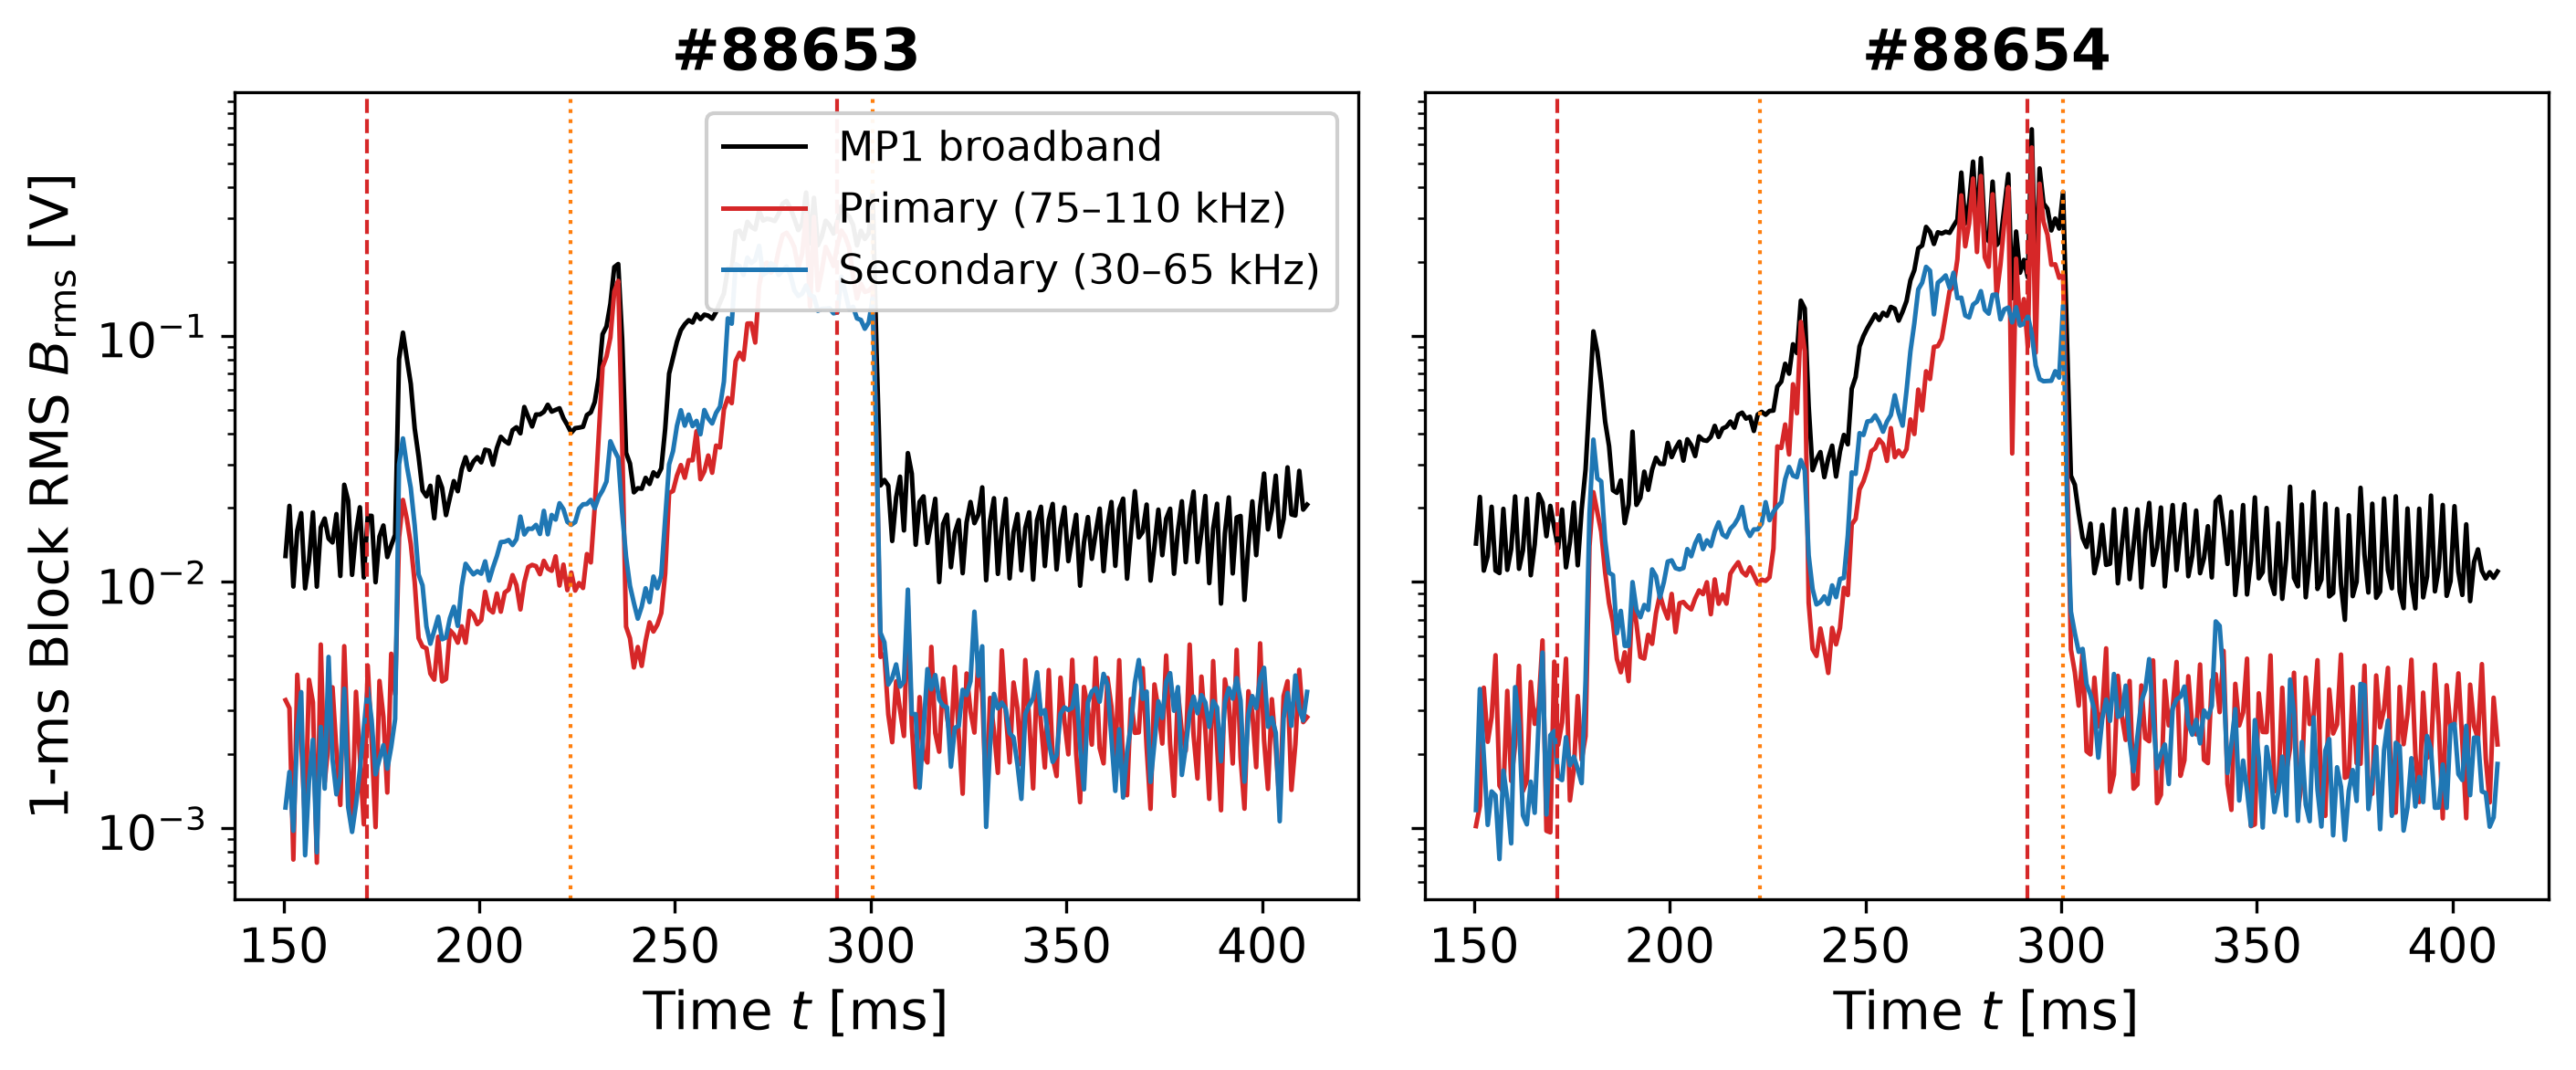
\includegraphics[width=0.90\textwidth]{Images/obj2_dynamics_and_structure/panels/fig_rms_vs_time_both_shots.png}
  \caption[MP1 RMS per millisecond, both shots]{Uncalibrated $1~\mathrm{ms}$-block MP1 RMS traces (log scale) across three frequency bands for \#88653 and \#88654.}
  \label{fig:rms_vs_time}
\end{figure}
Table~\ref{tab:discharge_phases} and Figures~\ref{fig:heating_timeline} and~\ref{fig:rms_vs_time} detailed discharge evolution across heating phases ($N = 1$ ECH-off transition per shot; vertical red and orange lines in Figure~\ref{fig:heating_timeline} marked the half-level ECH and NBIS10 crossings, where $291.2~\mathrm{ms}$ slightly preceded the $291.32~\mathrm{ms}$ \texttt{ECHRG500} half-drop). In shot \#88653, broadband MP1 RMS rose from $0.016~\mathrm{V}$ (pre-plasma) and $0.040~\mathrm{V}$ (ECH-only, $\gamma^2 = 0.158$) to $0.087~\mathrm{V}$ in early $\mathrm{ECH}+\mathrm{NBI}$ ($\gamma^2 = 0.931$; lines at $87.9, 139.6~\mathrm{kHz}$) and $0.274~\mathrm{V}$ in late $\mathrm{ECH}+\mathrm{NBI}$ ($\gamma^2 = 0.972$; lines at $40.0, 88.9~\mathrm{kHz}$). Amplitude peaked at $0.281~\mathrm{V}$ during $\mathrm{NBI}$-only ($\gamma^2 = 0.997$) before decaying to $0.054~\mathrm{V}$ post-heating. Both shots showed matching $1~\mathrm{ms}$ RMS traces (Figure~\ref{fig:rms_vs_time}: broadband along with Bessel-filtered $75\text{--}110~\mathrm{kHz}$ and $30\text{--}65~\mathrm{kHz}$ bands), including an \emph{unresolved} burst near $180~\mathrm{ms}$, a brief $235~\mathrm{ms}$ burst coinciding with an $I_p$ drop (Figure~\ref{fig:heating_timeline}), and sustained dual-band activity over $260\text{--}300.4~\mathrm{ms}$.

\begin{table}[H]
\centering
\small
\caption[Mode frequency shifts across ECH switch-off]{Mode frequency shifts across ECH switch-off.}
\label{tab:ech_switchoff_summary}
\sbox0{%
\begin{tabular}{lcccccccc}
\toprule
Quantity & \#88653 shift (kHz) & Sliding rank (-) & $p$ sliding (-) & Non-overlap rank (-) & $p$ non-overlap (-) & Surrogate $p$ (-) & \#88654 shift (kHz) & Same sign \\
\midrule
Secondary centroid & $-9.69$ & 0/54 & 0.018 & 0/5 & 0.167 & 0.004 & $-9.86$ & yes \\
Secondary dominant & $-10.74$ & 0/54 & 0.018 & 0/5 & 0.167 & 0.124 & $-12.70$ & yes \\
Primary centroid & $-3.94$ & 7/54 & 0.145 & 1/5 & 0.333 & 0.194 & $-8.55$ & yes \\
Primary dominant & $-5.86$ & 1/54 & 0.036 & 0/5 & 0.167 & 0.240 & $-11.72$ & yes \\
\bottomrule
\end{tabular}}
\ifdim\wd0>\textwidth\resizebox{\textwidth}{!}{\usebox0}\else\usebox0\fi
\par\smallskip{\footnotesize Two-sided rank $p$-values (500 surrogates for surrogate $p$); sliding placements overlap, whereas non-overlapping placements bound $p\ge 0.167$. One transition per shot.}
\end{table}
\begin{table}[H]
\centering
\small
\caption[Stored-energy slope change across ECH switch-off]{Stored-energy slope change across ECH switch-off.}
\label{tab:ech_wp_step}
\sbox0{%
\begin{tabular}{lcc}
\toprule
Fit window (ms) & \#88653 [95\,\% CI] (kW) & \#88654 [95\,\% CI] (kW) \\
\midrule
2 & $-54.3$ [$-61.6$, $-47.6$] & $-81.1$ [$-90.8$, $-71.3$] \\
5 & $-60.9$ [$-65.3$, $-56.9$] & $-68.3$ [$-79.0$, $-59.2$] \\
\bottomrule
\end{tabular}}
\ifdim\wd0>\textwidth\resizebox{\textwidth}{!}{\usebox0}\else\usebox0\fi
\par\smallskip{\footnotesize Post- minus pre-291.2~ms slope (negative: slower rise or faster decay of $W_p$; not absorbed gyrotron power); window-dependent; $95\,\%$ block-bootstrap confidence intervals (CI) in brackets. Post-ECH $n_e$ minimum in \#88653: $+0.40$~ms raw, $+0.36$~ms Savitzky--Golay smoothed (not evaluated for \#88654).}
\end{table}


\begin{figure}[H]
  \centering
  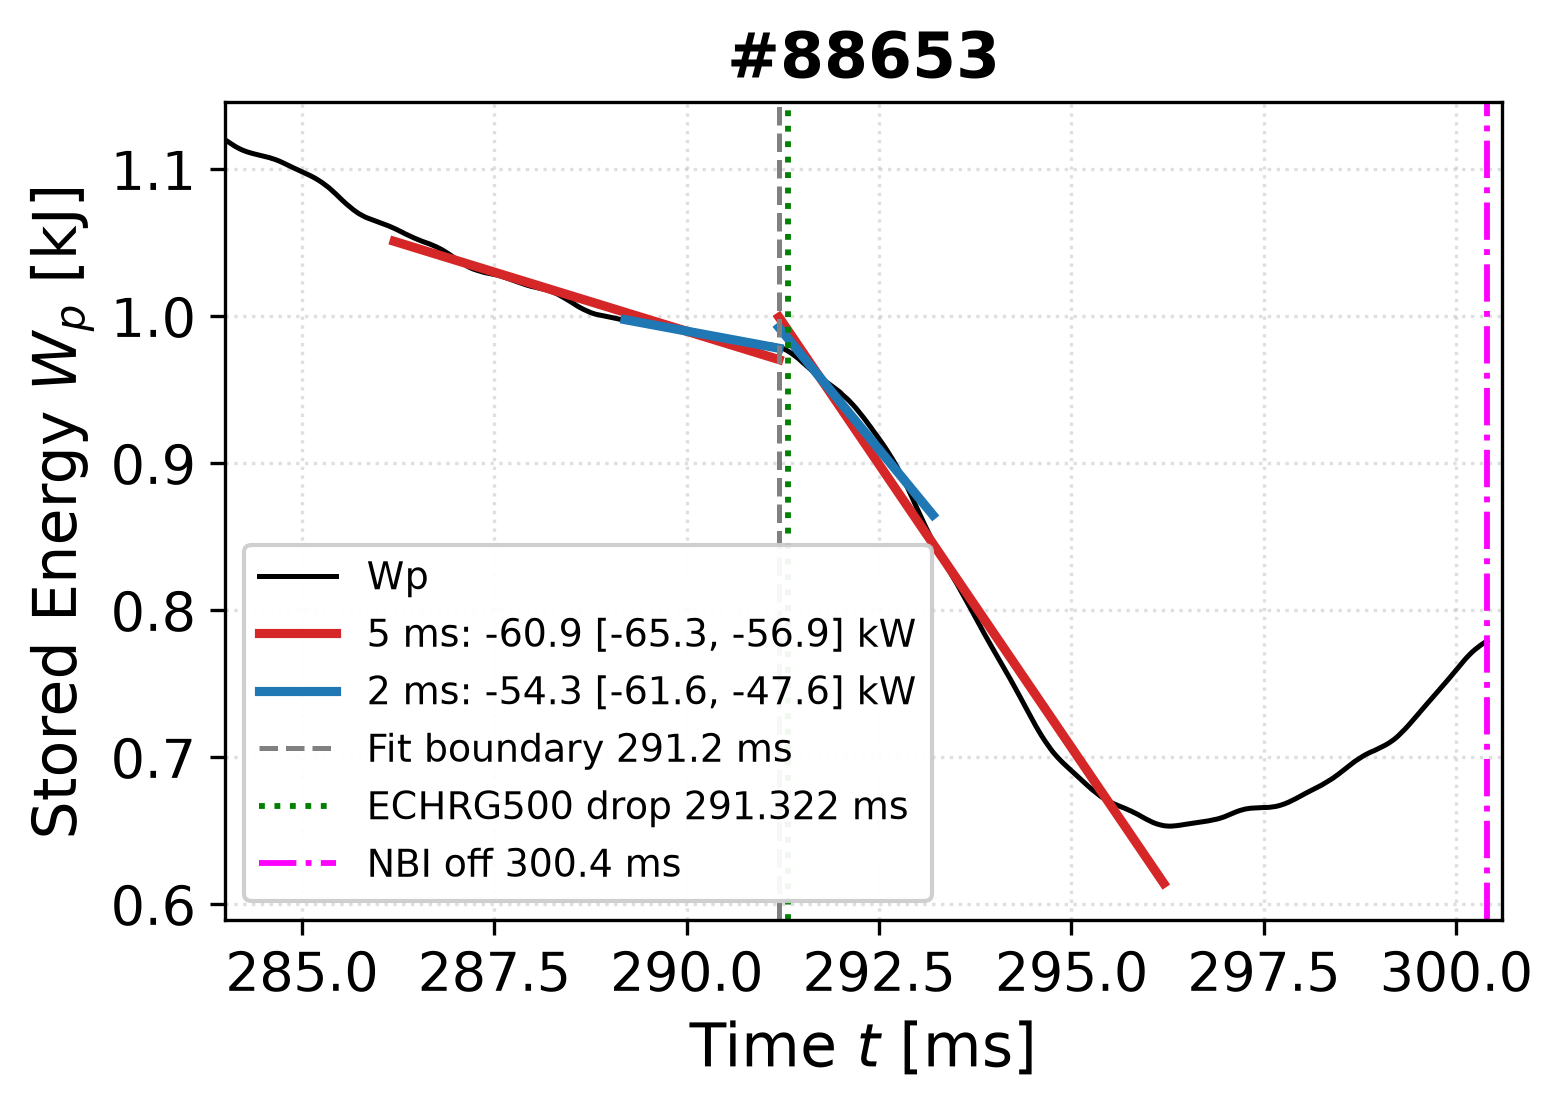
\includegraphics[width=0.49\textwidth]{Images/obj2_dynamics_and_structure/panels/fig_ech_wp_step_88653.png}
  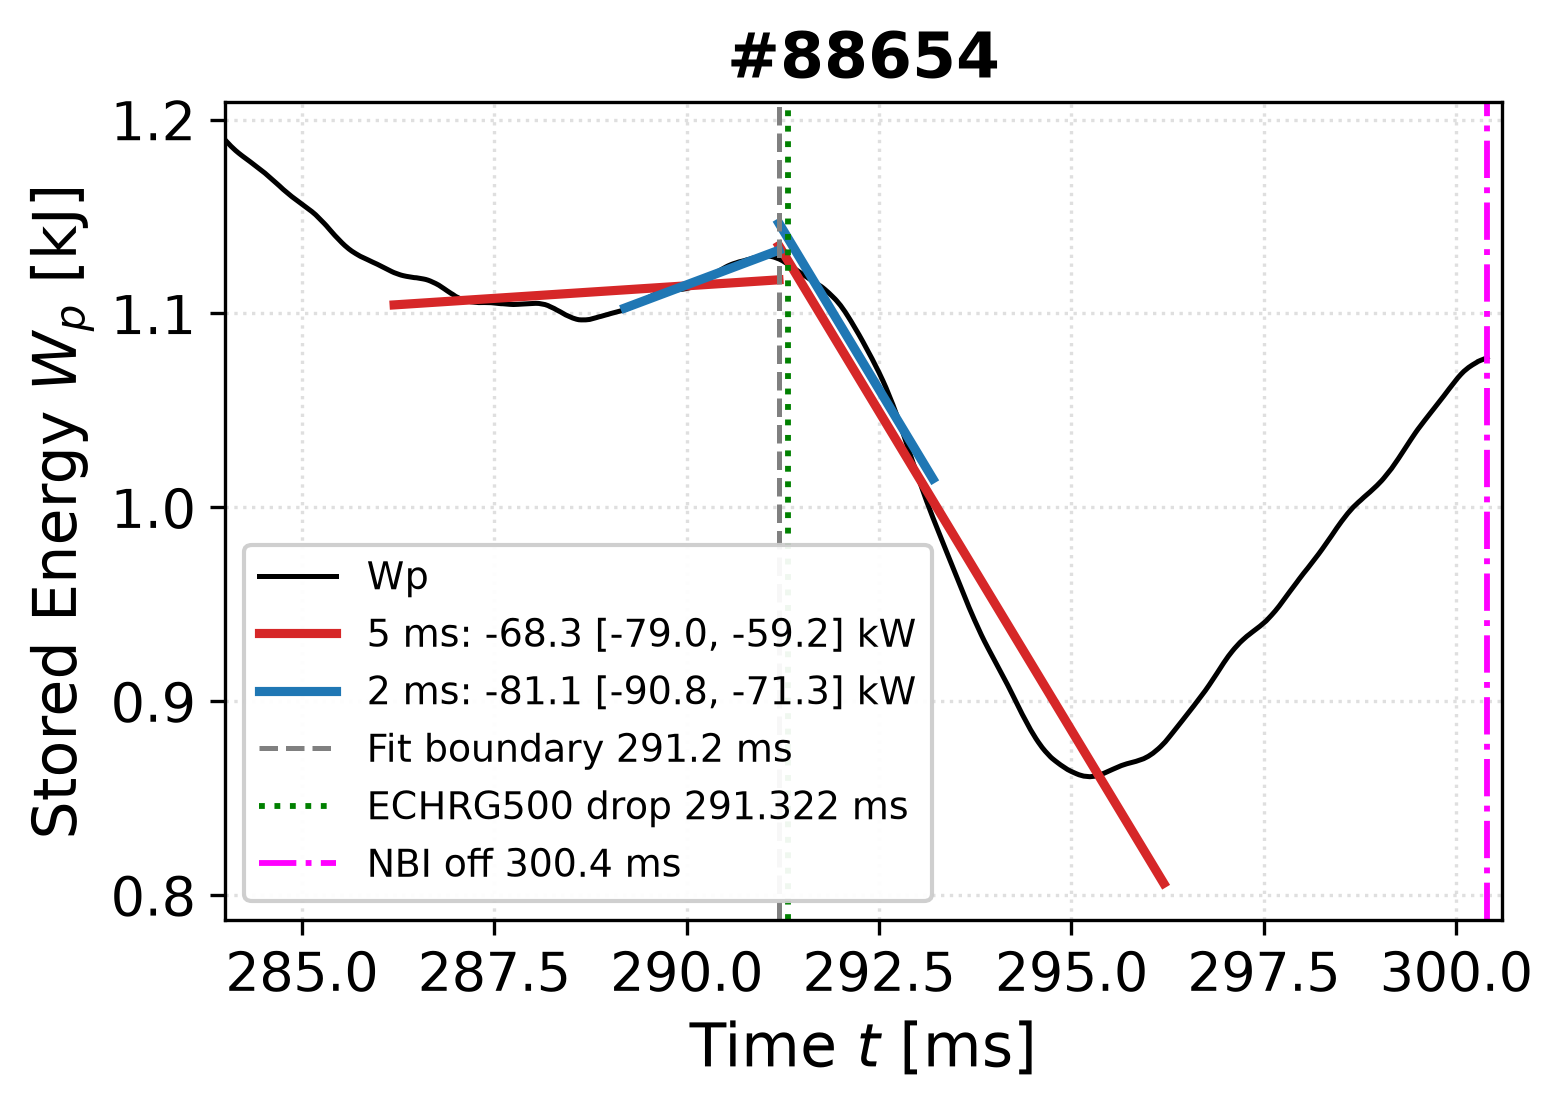
\includegraphics[width=0.49\textwidth]{Images/obj2_dynamics_and_structure/panels/fig_ech_wp_step_88654.png}
  \caption[Stored energy across ECH switch-off]{Stored energy $W_p$ across ECH switch-off ($291.2~\mathrm{ms}$) with $2$ and $5~\mathrm{ms}$ fits (\#88653, \#88654).}
  \label{fig:ech_wp_step}
\end{figure}

\begin{figure}[H]
  \centering
  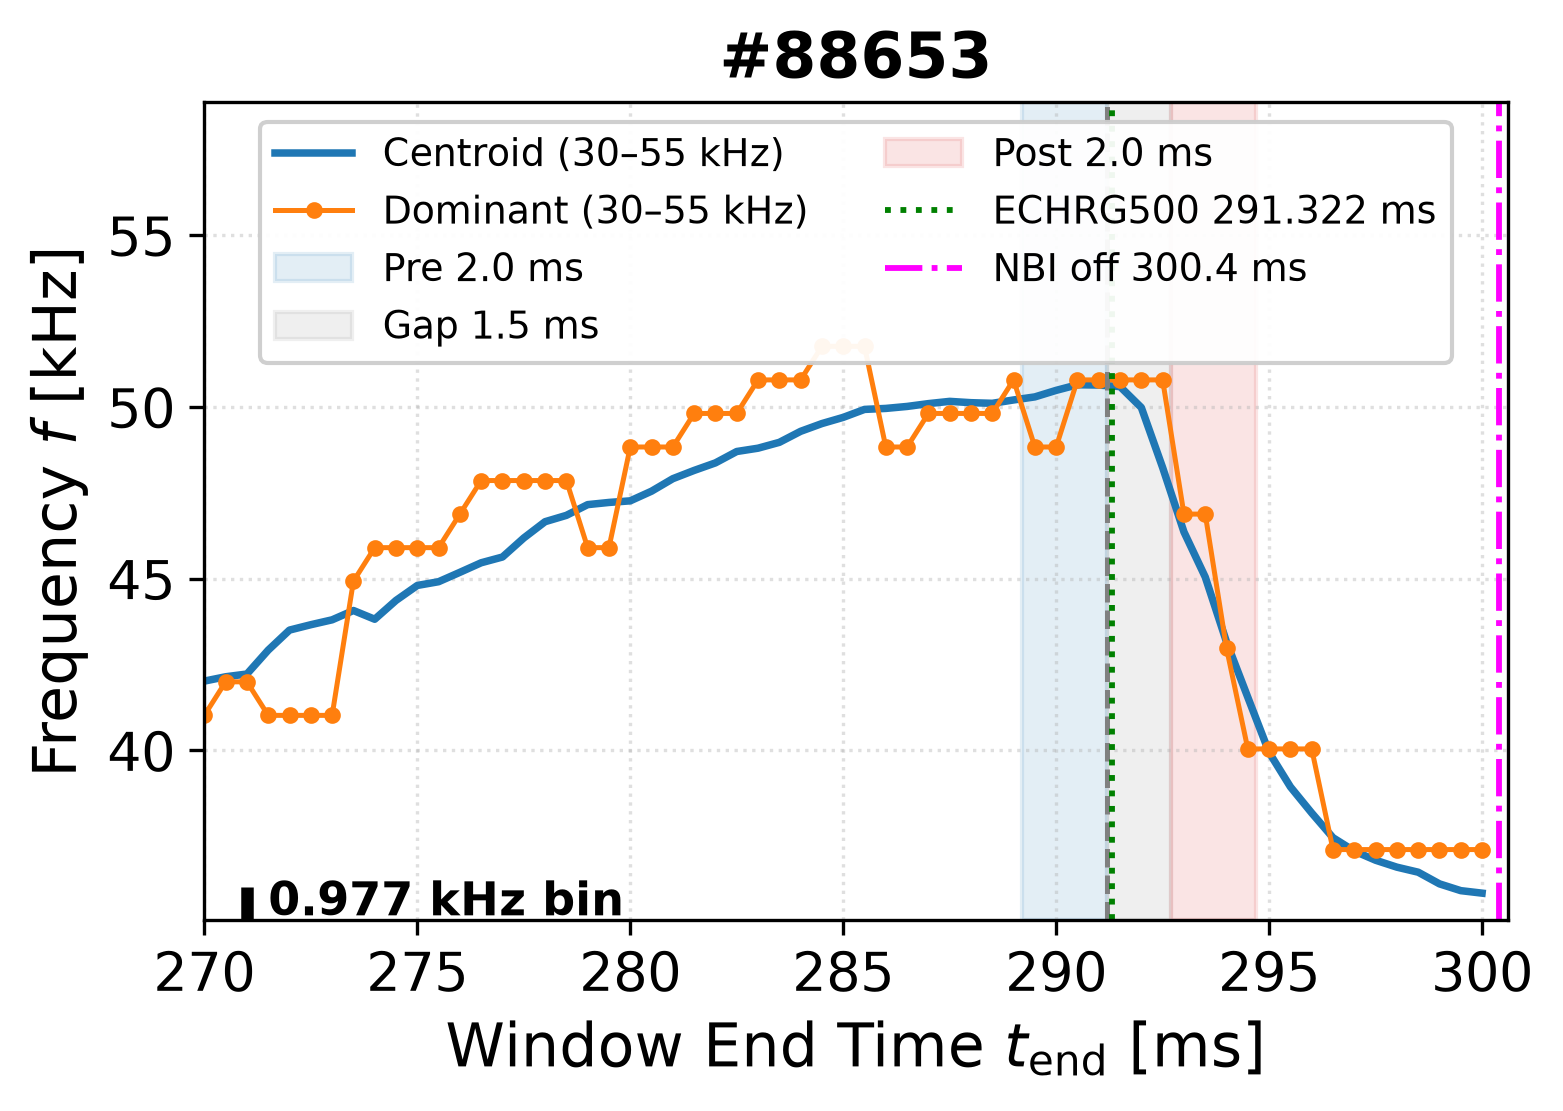
\includegraphics[width=0.49\textwidth]{Images/obj2_dynamics_and_structure/panels/fig_ech_secondary_freq_88653.png}
  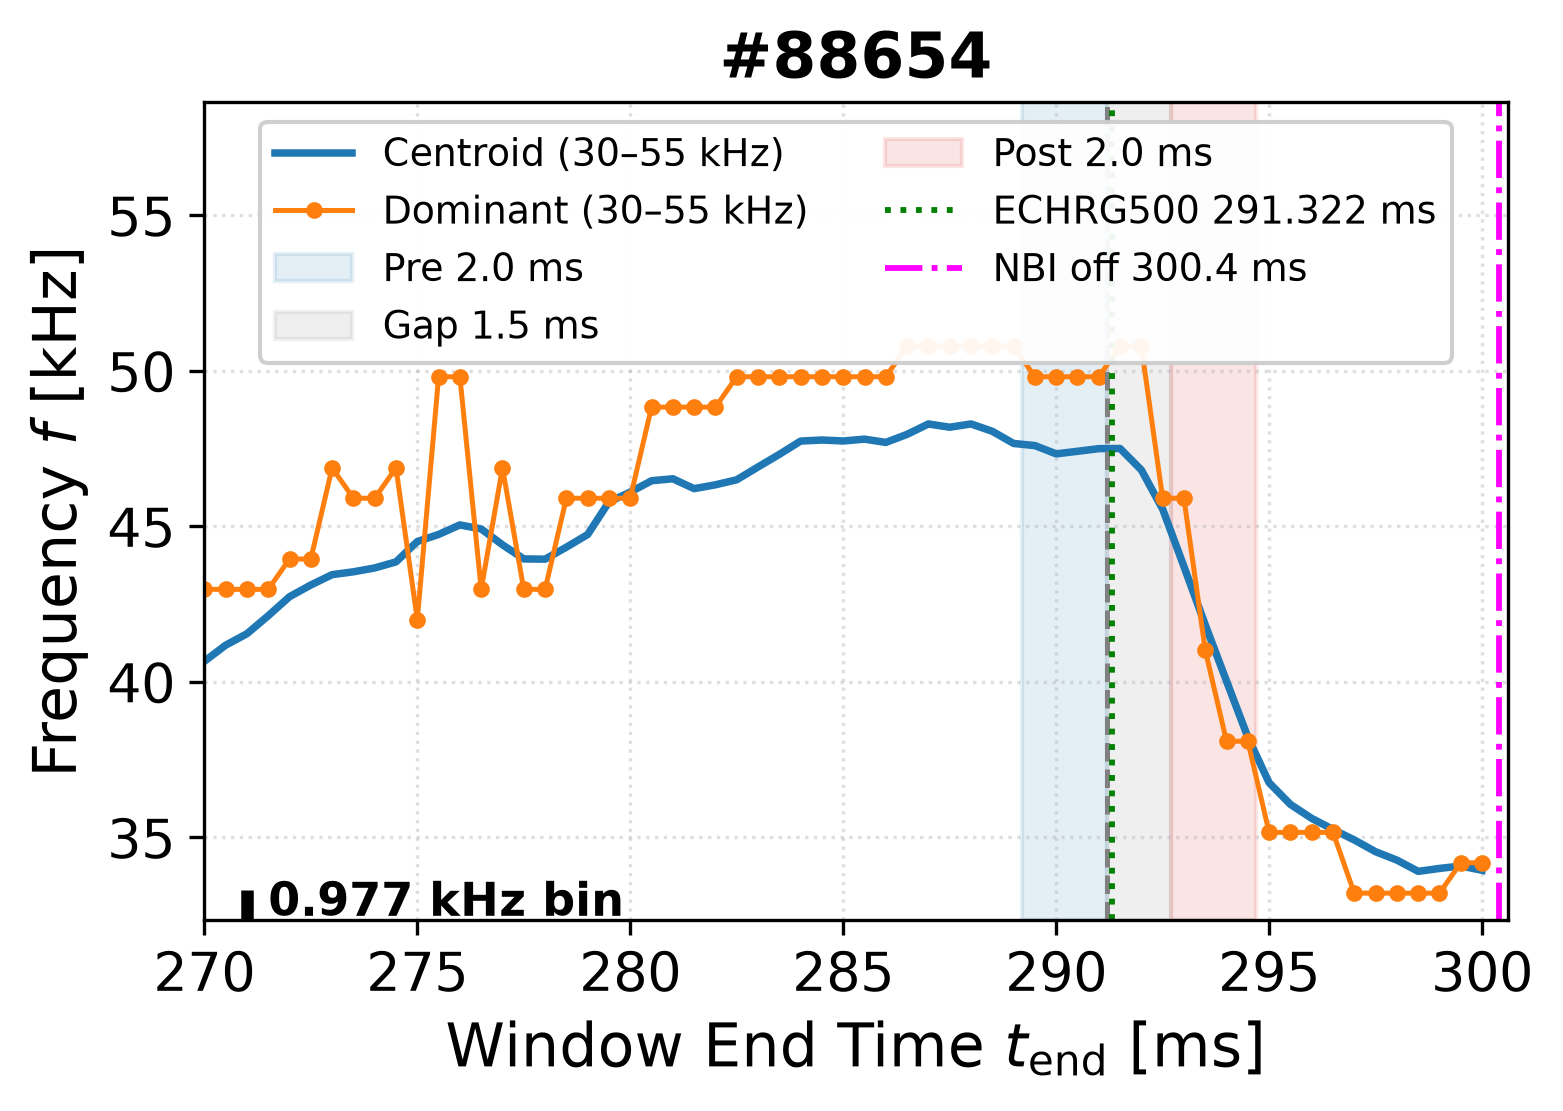
\includegraphics[width=0.49\textwidth]{Images/obj2_dynamics_and_structure/panels/fig_ech_secondary_freq_88654.png}
  \caption[Secondary-band frequency estimators]{Secondary-band ($30\text{--}55~\mathrm{kHz}$) centroid and dominant-bin frequencies across ECH switch-off for \#88653 and \#88654.}
  \label{fig:ech_secondary_freq}
\end{figure}
Tables~\ref{tab:ech_switchoff_summary} and~\ref{tab:ech_wp_step} and Figures~\ref{fig:ech_wp_step} and~\ref{fig:ech_secondary_freq} quantified the stored-energy slope change $\Delta(\mathrm{d}W_p/\mathrm{d}t)$ ($95~\%$ confidence interval, CI) and frequency shifts across $t_0 = 291.2~\mathrm{ms}$. In Figure~\ref{fig:ech_wp_step}, $\Delta(\mathrm{d}W_p/\mathrm{d}t)$ was negative and window-dependent in both shots: $-54.3~\mathrm{kW}$ ($[-61.6,\allowbreak -47.6]~\mathrm{kW}$ over $2~\mathrm{ms}$) and $-60.9~\mathrm{kW}$ ($[-65.3,\allowbreak -56.9]~\mathrm{kW}$ over $5~\mathrm{ms}$) in \#88653, versus $-81.1$ and $-68.3~\mathrm{kW}$ in \#88654. In \#88653, $n_e$ reached a local minimum $+0.40~\mathrm{ms}$ raw ($+0.36~\mathrm{ms}$ smoothed) after ECH-off. Physically, this $\mathrm{d}W_p/\mathrm{d}t$ step primarily reflected immediate removal of external ECH power at $t_0 = 291.2~\mathrm{ms}$ alongside any outward energy transport. In Figure~\ref{fig:ech_secondary_freq} (computed from trailing $2.0~\mathrm{ms}$ windows at $0.977~\mathrm{kHz}$ bins across shaded pre, $1.5~\mathrm{ms}$ gap, and post intervals) and Table~\ref{tab:ech_switchoff_summary}, the secondary centroid dropped by $-9.69~\mathrm{kHz}$ in \#88653 ($-9.86~\mathrm{kHz}$ in \#88654), exceeding all $54$ sliding ($p_{\mathrm{sliding}} = 0.018$) and $5$ non-overlapping ($p_{\mathrm{non\text{-}overlap}} \ge 0.167$) null placements with $p_{\mathrm{surr}} = 0.004$ (\emph{supported}). Because pre-transition upward chirping raised the baseline, this local $-9.69~\mathrm{kHz}$ step reconciled with the full-phase mean shift ($-6.1~\mathrm{kHz}$, Figure~\ref{fig:obj1_spectrogram}) and dominant peak step ($-7.8~\mathrm{kHz}$, Table~\ref{tab:mode_structure}). Discretized secondary peak shifts ($-10.74~\mathrm{kHz}$, $p_{\mathrm{surr}} = 0.124$) and primary-band shifts (centroid $-3.94~\mathrm{kHz}$, $p_{\mathrm{surr}} = 0.194$; dominant $-5.86~\mathrm{kHz}$, $p_{\mathrm{surr}} = 0.240$) remained \emph{inconclusive}. Moreover, a density-following fit ($f \propto n_e^{-\gamma}$ over $262\text{--}290$, $270\text{--}290$, and $275\text{--}291.2~\mathrm{ms}$) explained only $26.2~\%$, $21.3~\%$, and $17.8~\%$ of the drop, leaving the underlying mechanism \emph{unresolved}. This stronger sensitivity of the secondary band suggested a substantial $T_e$ or $\iota/2\pi$ role, consistent with ECH/ECCD tuning of core BAE and GAM frequencies~\cite{Varela2015,Varela2023,Yamamoto_2020,Zhong2024,Adulsiriswad_2024}.


\subsection[Objective 2 -- EPM-Heating Correlation and Statistical Metrics]{Objective 2 -- EPM-Heating Correlation\\ and Statistical Metrics}
\label{subsec:obj2}

\subsubsection{Envelope Correlations with \texorpdfstring{$I_p$, $W_p$, $n_e$}{Ip, Wp, ne}}
\label{subsubsec:obj2_envelope}

\begin{figure}[H]
  \centering
  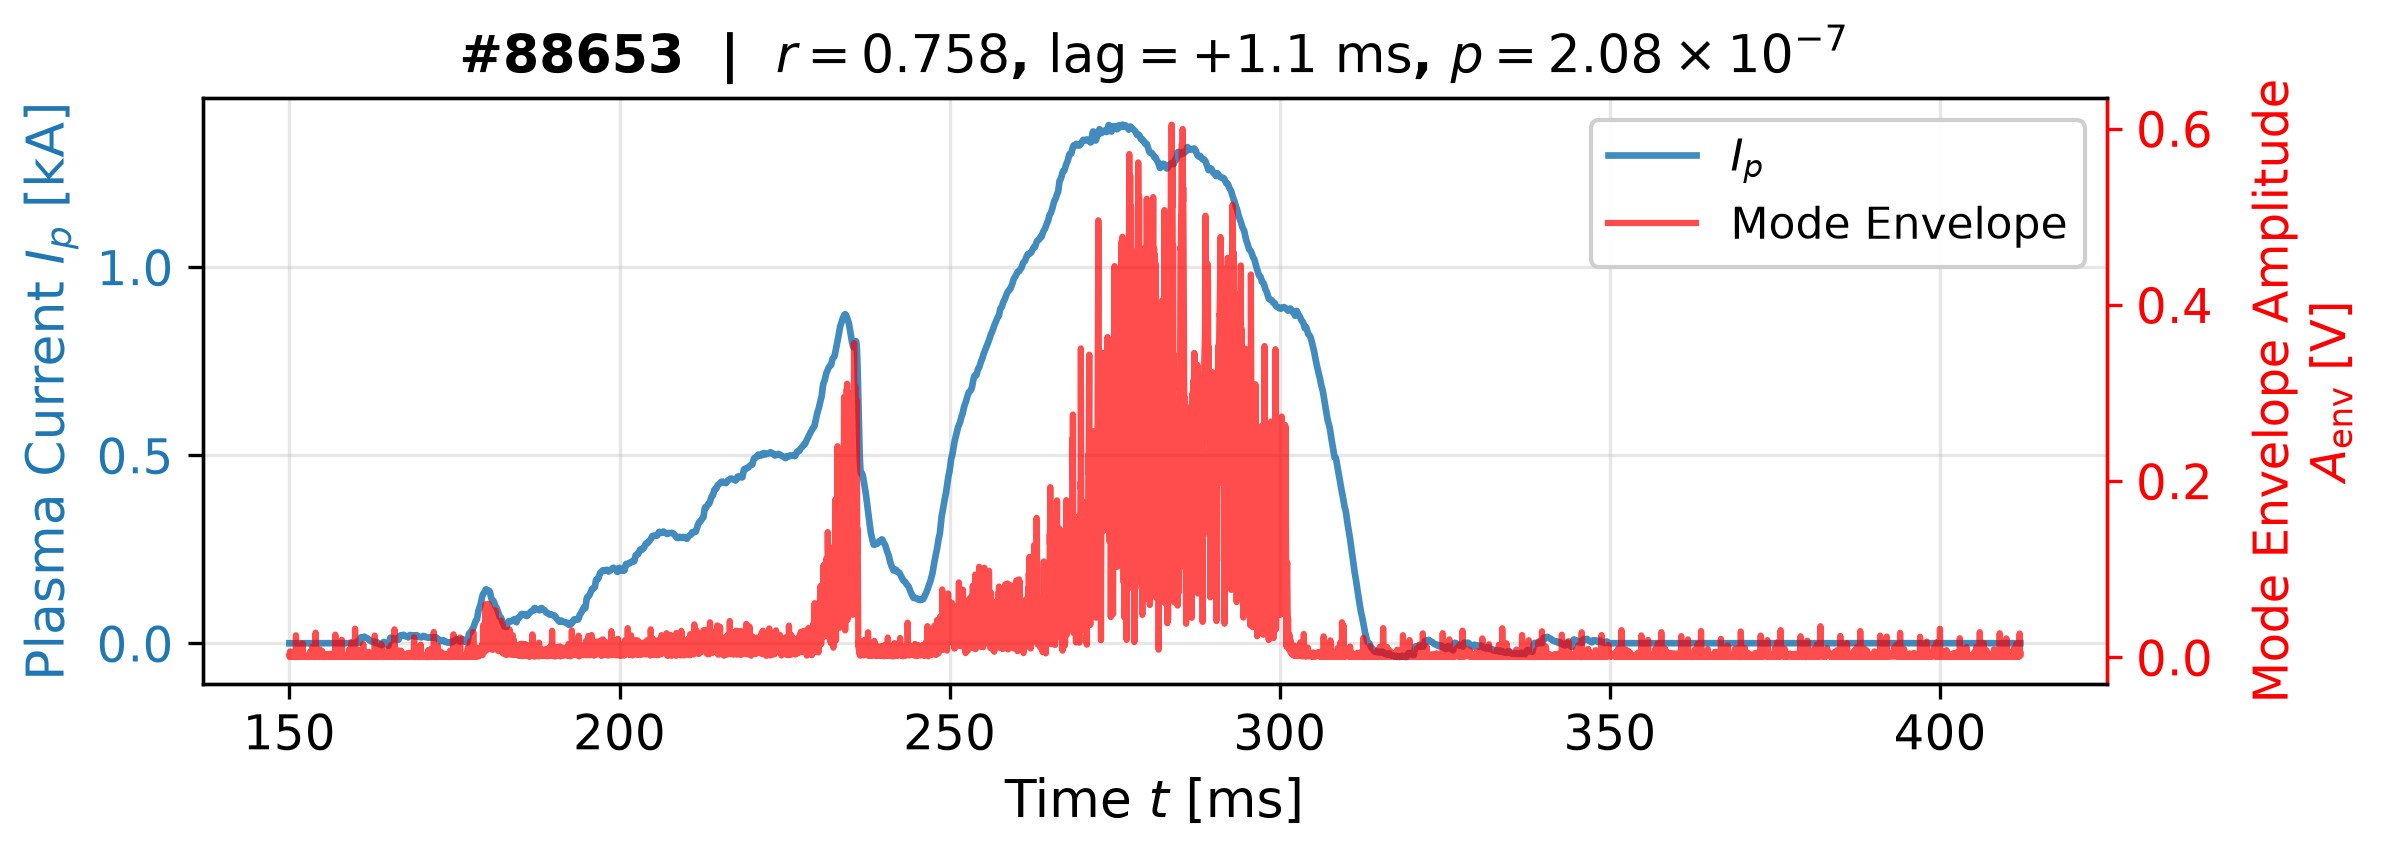
\includegraphics[width=0.86\textwidth]{Images/obj2_dynamics_and_structure/panels/mhd_analysis_objective2_88653_80_120kHz_panel1_correlation_plasma_current_ip15_vs_mode.png}
  \caption[Primary mode envelope correlation with plasma current]{Primary mode envelope ($80\text{--}120~\mathrm{kHz}$) versus plasma current $I_p$ over the full record (\#88653).}
  \label{fig:obj2_envelope_ip}
  \vspace{0.25em}
  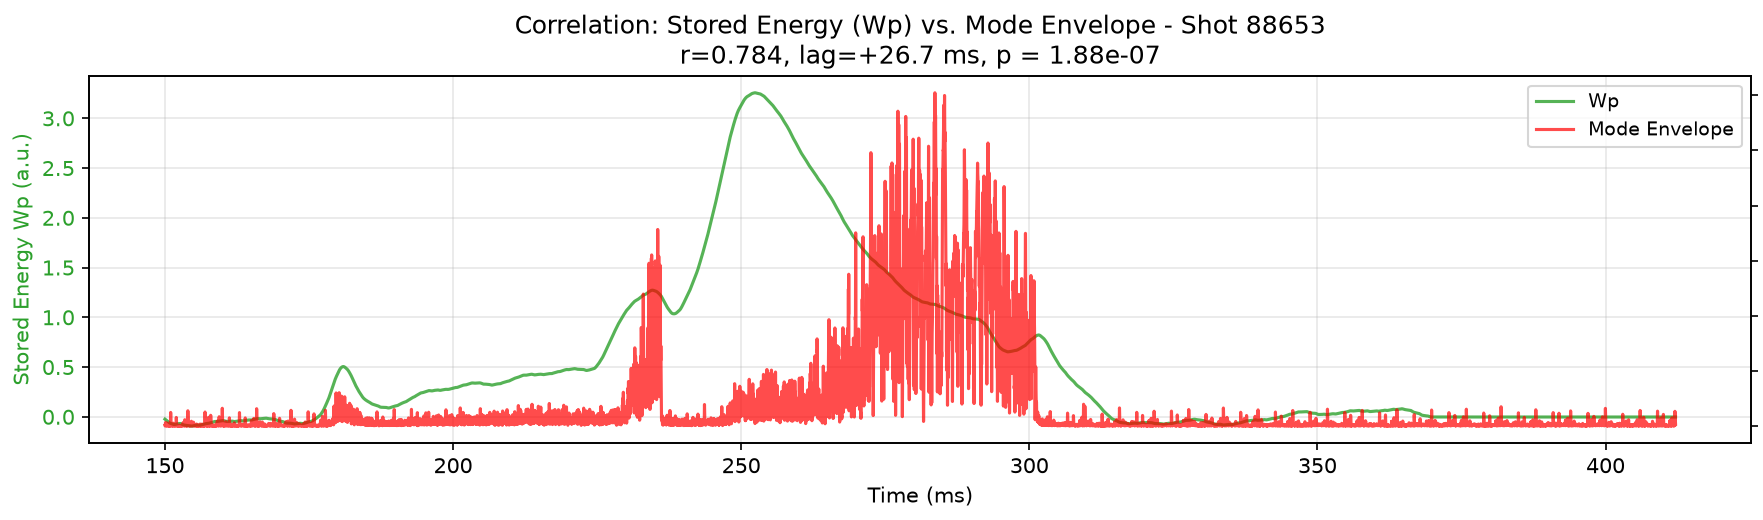
\includegraphics[width=0.86\textwidth]{Images/obj2_dynamics_and_structure/panels/mhd_analysis_objective2_88653_80_120kHz_panel2_correlation_stored_energy_wp_vs_mode_env.png}
  \caption[Primary mode envelope correlation with stored energy]{Primary mode envelope ($80\text{--}120~\mathrm{kHz}$) versus stored energy $W_p$ over the full record (\#88653).}
  \label{fig:obj2_envelope_wp}
  \vspace{0.25em}
  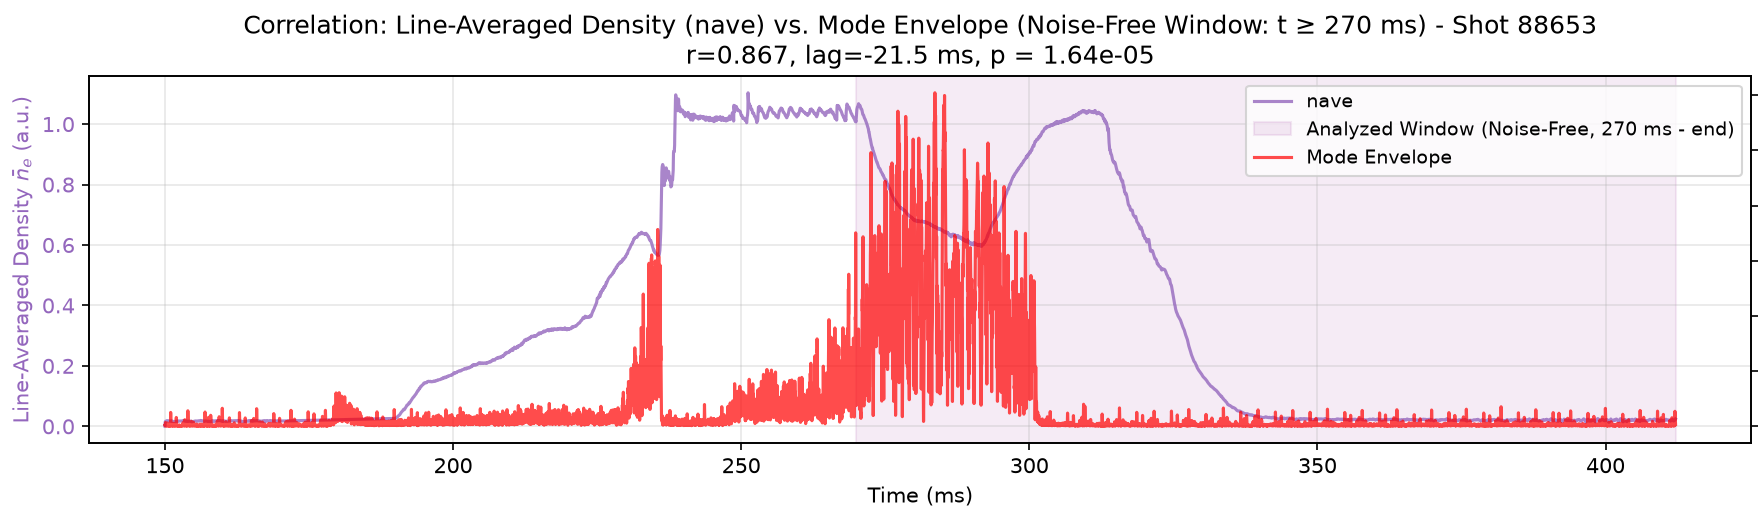
\includegraphics[width=0.86\textwidth]{Images/obj2_dynamics_and_structure/panels/mhd_analysis_objective2_88653_80_120kHz_panel3_correlation_line_averaged_density_nave_v.png}
  \caption[Primary mode envelope correlation with electron density]{Primary mode envelope ($80\text{--}120~\mathrm{kHz}$) versus line-averaged density $n_e$ ($t \geq 270.0~\mathrm{ms}$, \#88653).}
  \label{fig:obj2_envelope_ne}
\end{figure}
Figures~\ref{fig:obj2_envelope_ip}, \ref{fig:obj2_envelope_wp}, and~\ref{fig:obj2_envelope_ne} and Table~\ref{tab:obj2_both_shots} reported lagged cross-correlations of the $80\text{--}120~\mathrm{kHz}$ primary-mode envelope against $I_p$, $W_p$, and $n_e$. In shot \#88653, all three proxies exceeded $|r| > 0.70$. Specifically, $I_p$ yielded $r = 0.7575$ at lag $+1.10~\mathrm{ms}$ ($N_{\mathrm{eff}} = 34.1$, $p = 2.08 \times 10^{-7}$), and $W_p$ yielded $r = 0.7840$ at $+26.70~\mathrm{ms}$ after the $252~\mathrm{ms}$ peak ($N_{\mathrm{eff}} = 30.9$, $p = 1.88 \times 10^{-7}$). Over $t \ge 270~\mathrm{ms}$, $n_e$ yielded $r = 0.8666$ at lag $-21.50~\mathrm{ms}$ ($N_{\mathrm{eff}} = 15.8$, $p = 1.64 \times 10^{-5}$). Replicate shot \#88654 matched all lag directions ($+1.30$, $+28.90$, $-21.20~\mathrm{ms}$), with $n_e$ clearing threshold ($r = 0.7099$, $N_{\mathrm{eff}} = 22.9$) while $I_p$ ($0.6555$) and $W_p$ ($0.6590$) stayed below $0.70$. Because these traces shared heating ramps and collapsed to near-zero partial correlation under ECH-step control ($r = +0.0609, +0.0023$ for envelope; $+0.076, -0.074$ for frequency), macroscopic correlations remained \emph{suggestive} rather than causal.

\begin{table}[H]
\centering
\footnotesize
\setlength{\tabcolsep}{4pt}
\renewcommand{\arraystretch}{1.15}
\caption[Primary-mode correlations and scaling models for both shots]{Primary-mode correlations and scaling models for both shots.}
\label{tab:obj2_both_shots}
\begin{tabular}{lcccccccc}
\toprule
 & \multicolumn{4}{c}{\#88653} & \multicolumn{4}{c}{\#88654} \\
\cmidrule(lr){2-5}\cmidrule(lr){6-9}
Quantity & \shortstack{Pearson\\$r$ (-)} & $N_{\rm eff}$ (-) & \shortstack{Lag\\(ms)} & $p$ (-) & \shortstack{Pearson\\$r$ (-)} & $N_{\rm eff}$ (-) & \shortstack{Lag\\(ms)} & $p$ (-) \\
\midrule
$I_p$ & 0.7575 & 34.1 & $+1.10$ & $2.08\times10^{-7}$ & 0.6555 & 46.8 & $+1.30$ & $6.10\times10^{-7}$ \\
$W_p$ & 0.7840 & 30.9 & $+26.70$ & $1.88\times10^{-7}$ & 0.6590 & 42.3 & $+28.90$ & $1.89\times10^{-6}$ \\
\shortstack[l]{$n_e$ (270 ms\\to end)} & 0.8666 & 15.8 & $-21.50$ & $1.64\times10^{-5}$ & 0.7099 & 22.9 & $-21.20$ & $1.55\times10^{-4}$ \\
\midrule
\multicolumn{9}{l}{\textbf{Candidate Frequency Scaling Models (Best Fit in Burst Window)}} \\
\midrule
\shortstack[l]{Primary best\\scaling $r$} & \multicolumn{4}{c}{\shortstack{BAE Coupled ($\sqrt{v_A^2 + c_s^2}$):\\$+0.545$ ($p_{\mathrm{adj}}=0.139$)}} & \multicolumn{4}{c}{\shortstack{Stored Energy ($W_p$):\\$+0.604$ ($p_{\mathrm{adj}}=0.099$)}} \\
\shortstack[l]{Secondary best\\scaling $r$} & \multicolumn{4}{c}{\shortstack{BAE Acoustic ($\sqrt{T_e}$):\\$+0.848$ ($p_{\mathrm{adj}}=0.162$)}} & \multicolumn{4}{c}{\shortstack{Stored Energy ($W_p$):\\$+0.343$ ($p_{\mathrm{adj}}=0.157$)}} \\
\midrule
\multicolumn{9}{l}{\textbf{ECH-Step-Controlled Partial Correlations}} \\
\midrule
\shortstack[l]{Envelope, ECH-step-\\controlled $r$} & \multicolumn{4}{c}{$+0.0609$} & \multicolumn{4}{c}{$+0.0023$} \\
\shortstack[l]{Frequency, ECH-step-\\controlled $r$} & \multicolumn{4}{c}{$+0.076$} & \multicolumn{4}{c}{$-0.074$} \\
\bottomrule
\end{tabular}
\par\smallskip Primary band ($80\text{--}120$~kHz) correlations evaluated per discharge (\#88654 serves as an independent same-direction check); secondary band ($40\text{--}80$~kHz) best scaling models are listed alongside primary scaling for completeness. Lag denotes peak cross-correlation offset; $p$-values use autocorrelation-adjusted $N_{\rm eff}$. Correlations remain \emph{suggestive} at most due to shared heating ramps and limited $N_{\rm eff}$.
\end{table}


\subsubsection{Verification of Relative \texorpdfstring{$T_e$}{Te} Proxy and Frequency Scaling Models}
\label{subsubsec:obj2_scaling}

To test whether low-pass filtered ECE traces followed slow thermal evolution, baseline-subtracted non-saturated channels were filtered with a 4th-order zero-phase Butterworth LPF ($f_c = 30~\mathrm{Hz}$ SOS), removing ${\sim}800~\mathrm{Hz}$ sawtooth and MHD modulations. Figure~\ref{fig:ece_te_verification}(a) compared these normalized $30~\mathrm{Hz}$ low-pass ECE signals (\texttt{ECE12FAST} and \texttt{ECE9FAST}) against stored energy $W_p(t)$, line-averaged density $n_e(t)$, and the diamagnetic temperature proxy $T_{e,\mathrm{dia}} \propto W_p/n_e$ over $240.0\text{--}305.0~\mathrm{ms}$ across density pump-out ($270.0\text{--}291.2~\mathrm{ms}$) and ECH shut-off ($291.2~\mathrm{ms}$).

\begin{figure}[H]
  \centering
  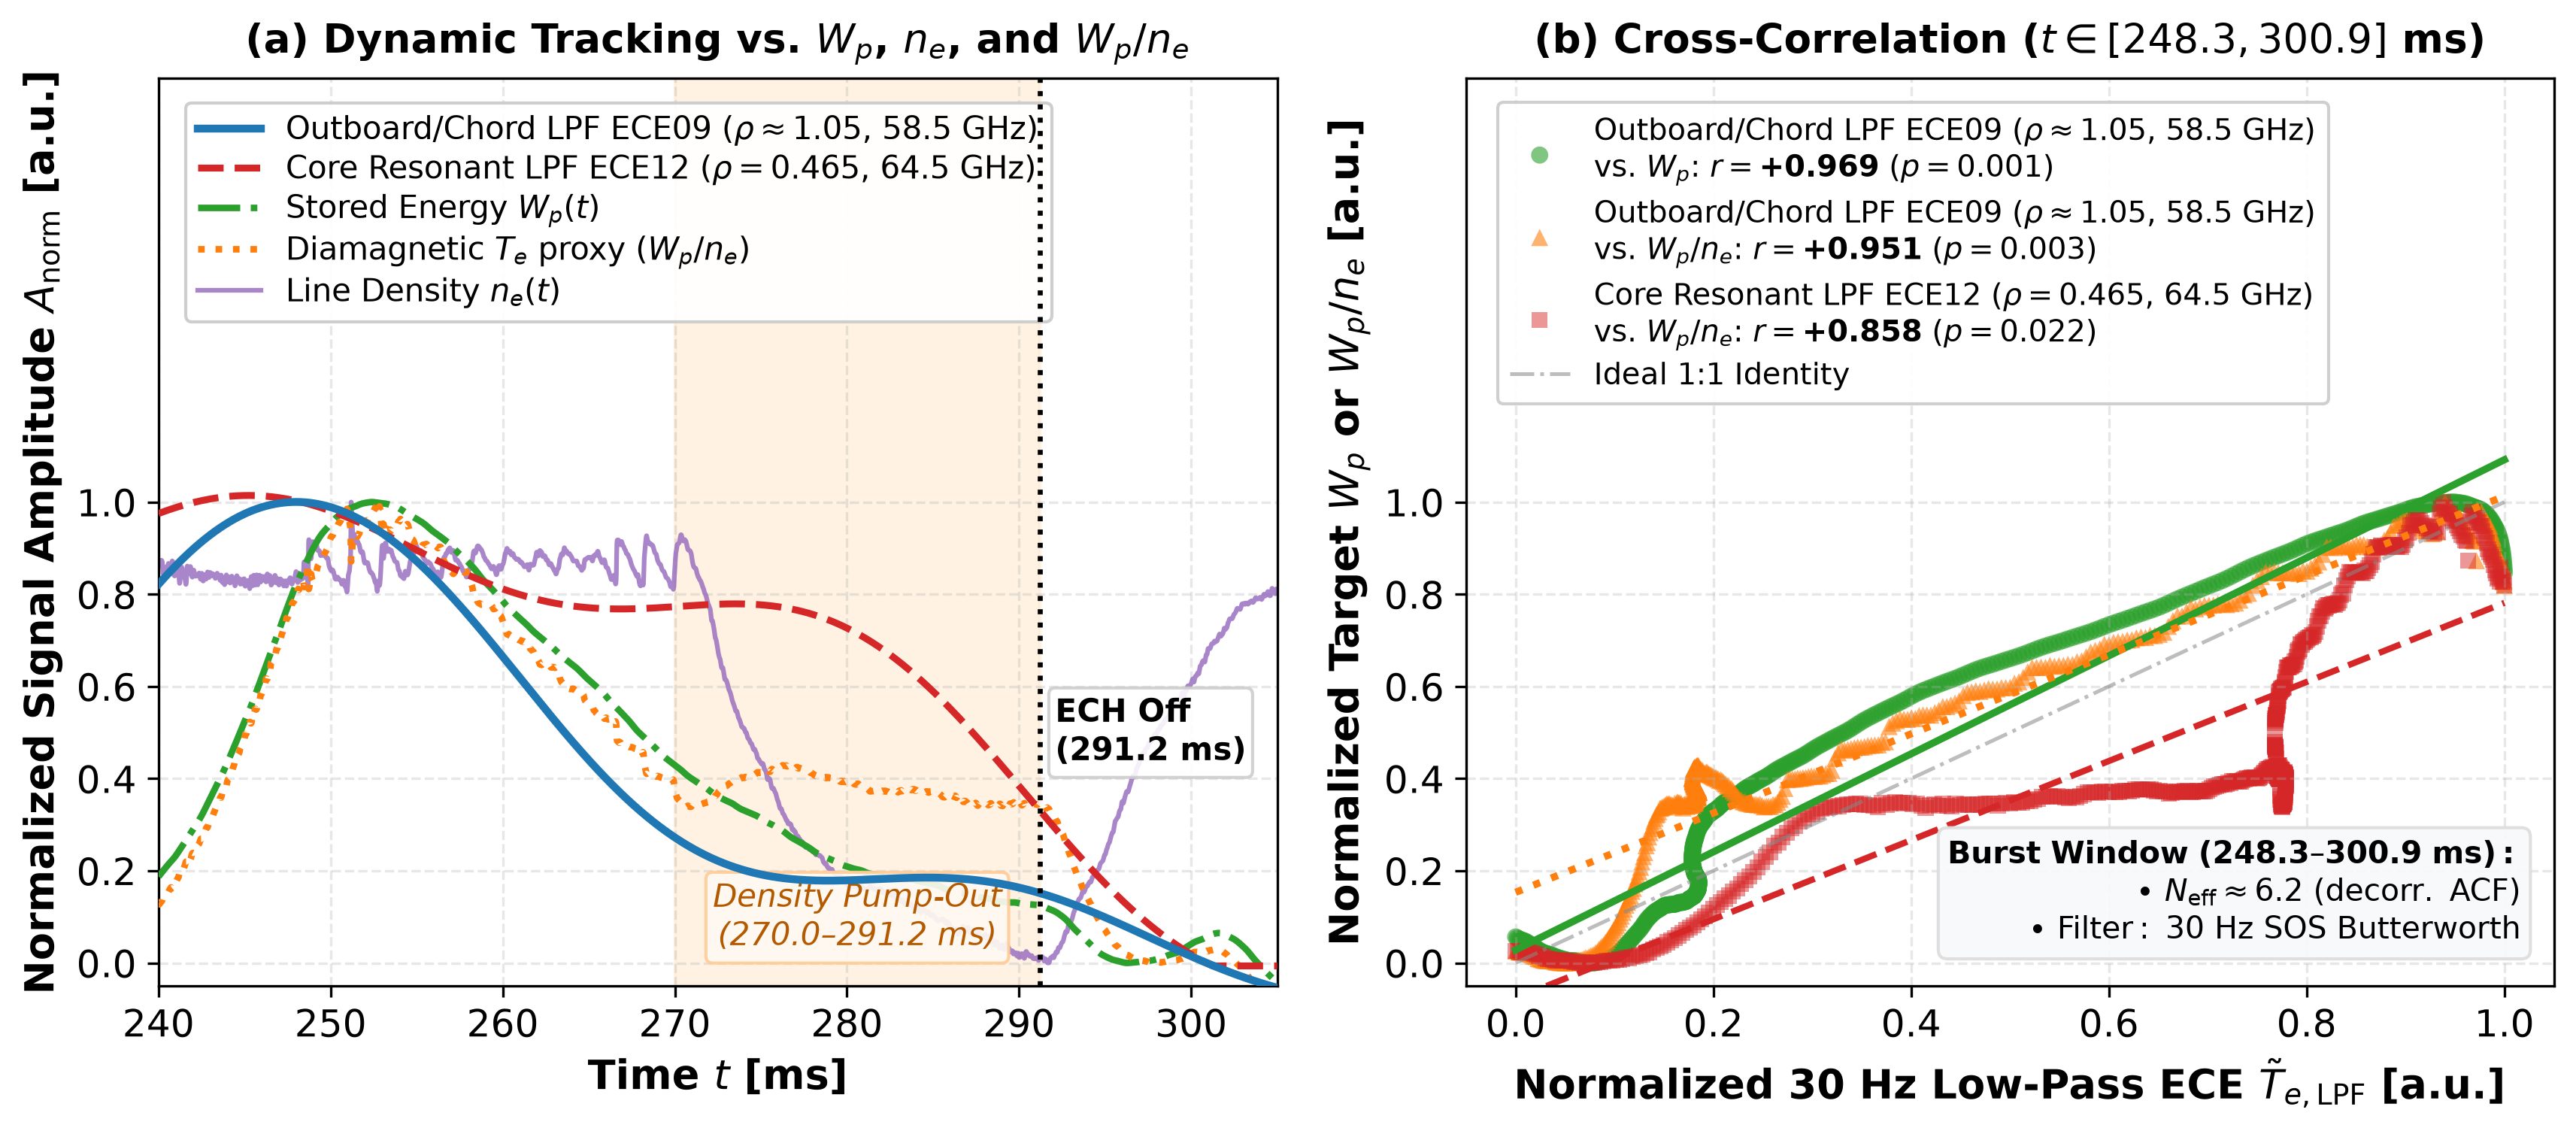
\includegraphics[width=0.98\textwidth]{Images/obj2_dynamics_and_structure/mhd_ece_lpf_te_verification_88653.png}
  \caption[Verification of relative $T_e$ proxy via low-pass filtered ECE]{Verification of relative $T_e$ proxy in shot \#88653: (a)~normalized $30~\mathrm{Hz}$ low-pass ECE traces and (b)~burst-window regressions.}
  \label{fig:ece_te_verification}
\end{figure}

Within the active burst window ($248.3\text{--}300.9~\mathrm{ms}$, Figure~\ref{fig:ece_te_verification}(b)), the optically thick resonant core channel \texttt{ECE12FAST} ($64.5~\mathrm{GHz}$, $\rho = 0.465$) served as the localized core thermal proxy, tracking both $W_p/n_e$ ($r = +0.858$, $p = 0.022$) and $W_p$ ($r = +0.811$). By contrast, \texttt{ECE9FAST} ($58.5~\mathrm{GHz}$, $\rho \approx 1.05$) represented a non-saturated outboard boundary / chord-integrated radiometer channel rather than a localized core measurement. Its $30~\mathrm{Hz}$ low-pass filtered intensity nonetheless tracked global stored energy $W_p$ ($r = +0.969$, $p = 0.001$, $N_{\mathrm{eff}} \approx 6.2$; $r = +0.805$ full shot) and $W_p/n_e$ ($r = +0.951$, $p = 0.003$). This reflected optically thin X2 emission capturing wall-reflected and chord-averaged bulk plasma behavior. Within the modest effective sample size ($N_{\mathrm{eff}} \approx 6.2$), this quantitative consistency supported $30~\mathrm{Hz}$ low-pass filtered ECE as a relative thermal evolution proxy.

\begin{figure}[H]
  \centering
  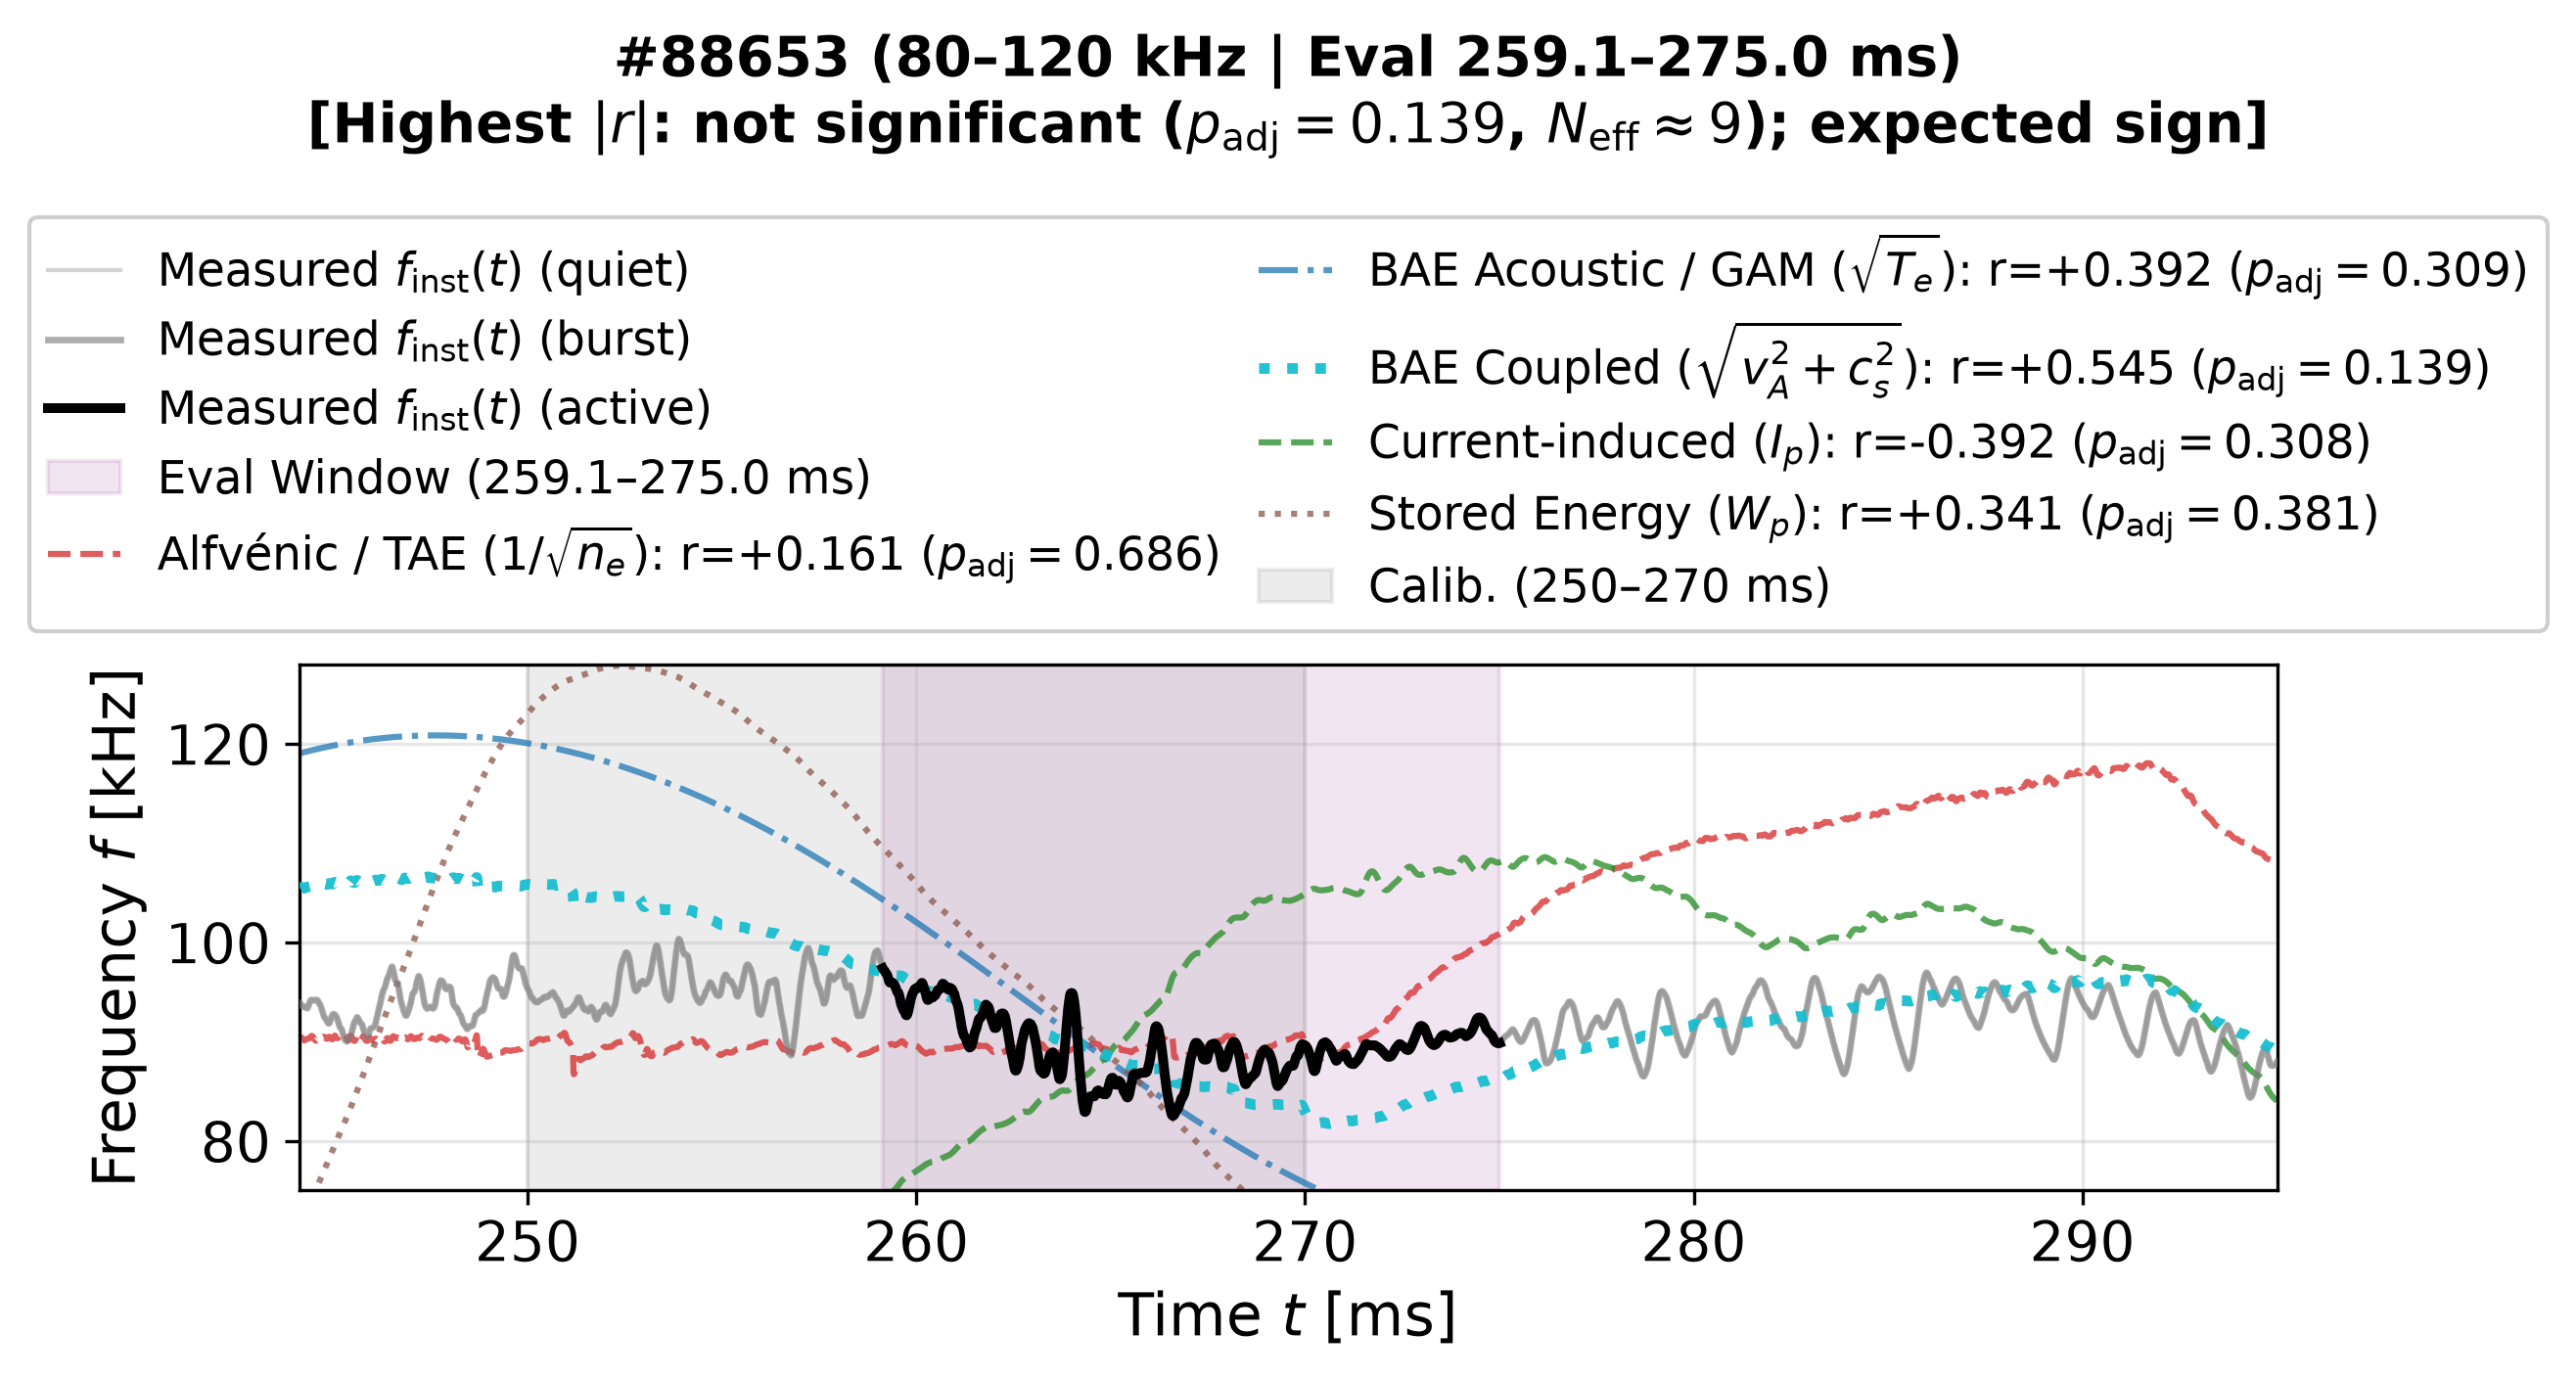
\includegraphics[width=0.92\textwidth]{Images/obj2_dynamics_and_structure/panels/mhd_analysis_objective2_heating_88653_80_120kHz_panel4_energetic_particle_mode_identification_m.png}
  \caption[Primary mode frequency response to candidate scaling models]{Primary mode ($80\text{--}120~\mathrm{kHz}$) frequency versus $30~\mathrm{Hz}$ LPF scaling models ($259.1\text{--}275.0~\mathrm{ms}$, \#88653).}
  \label{fig:obj2_epm_models_primary}
  \vspace{0.3em}
  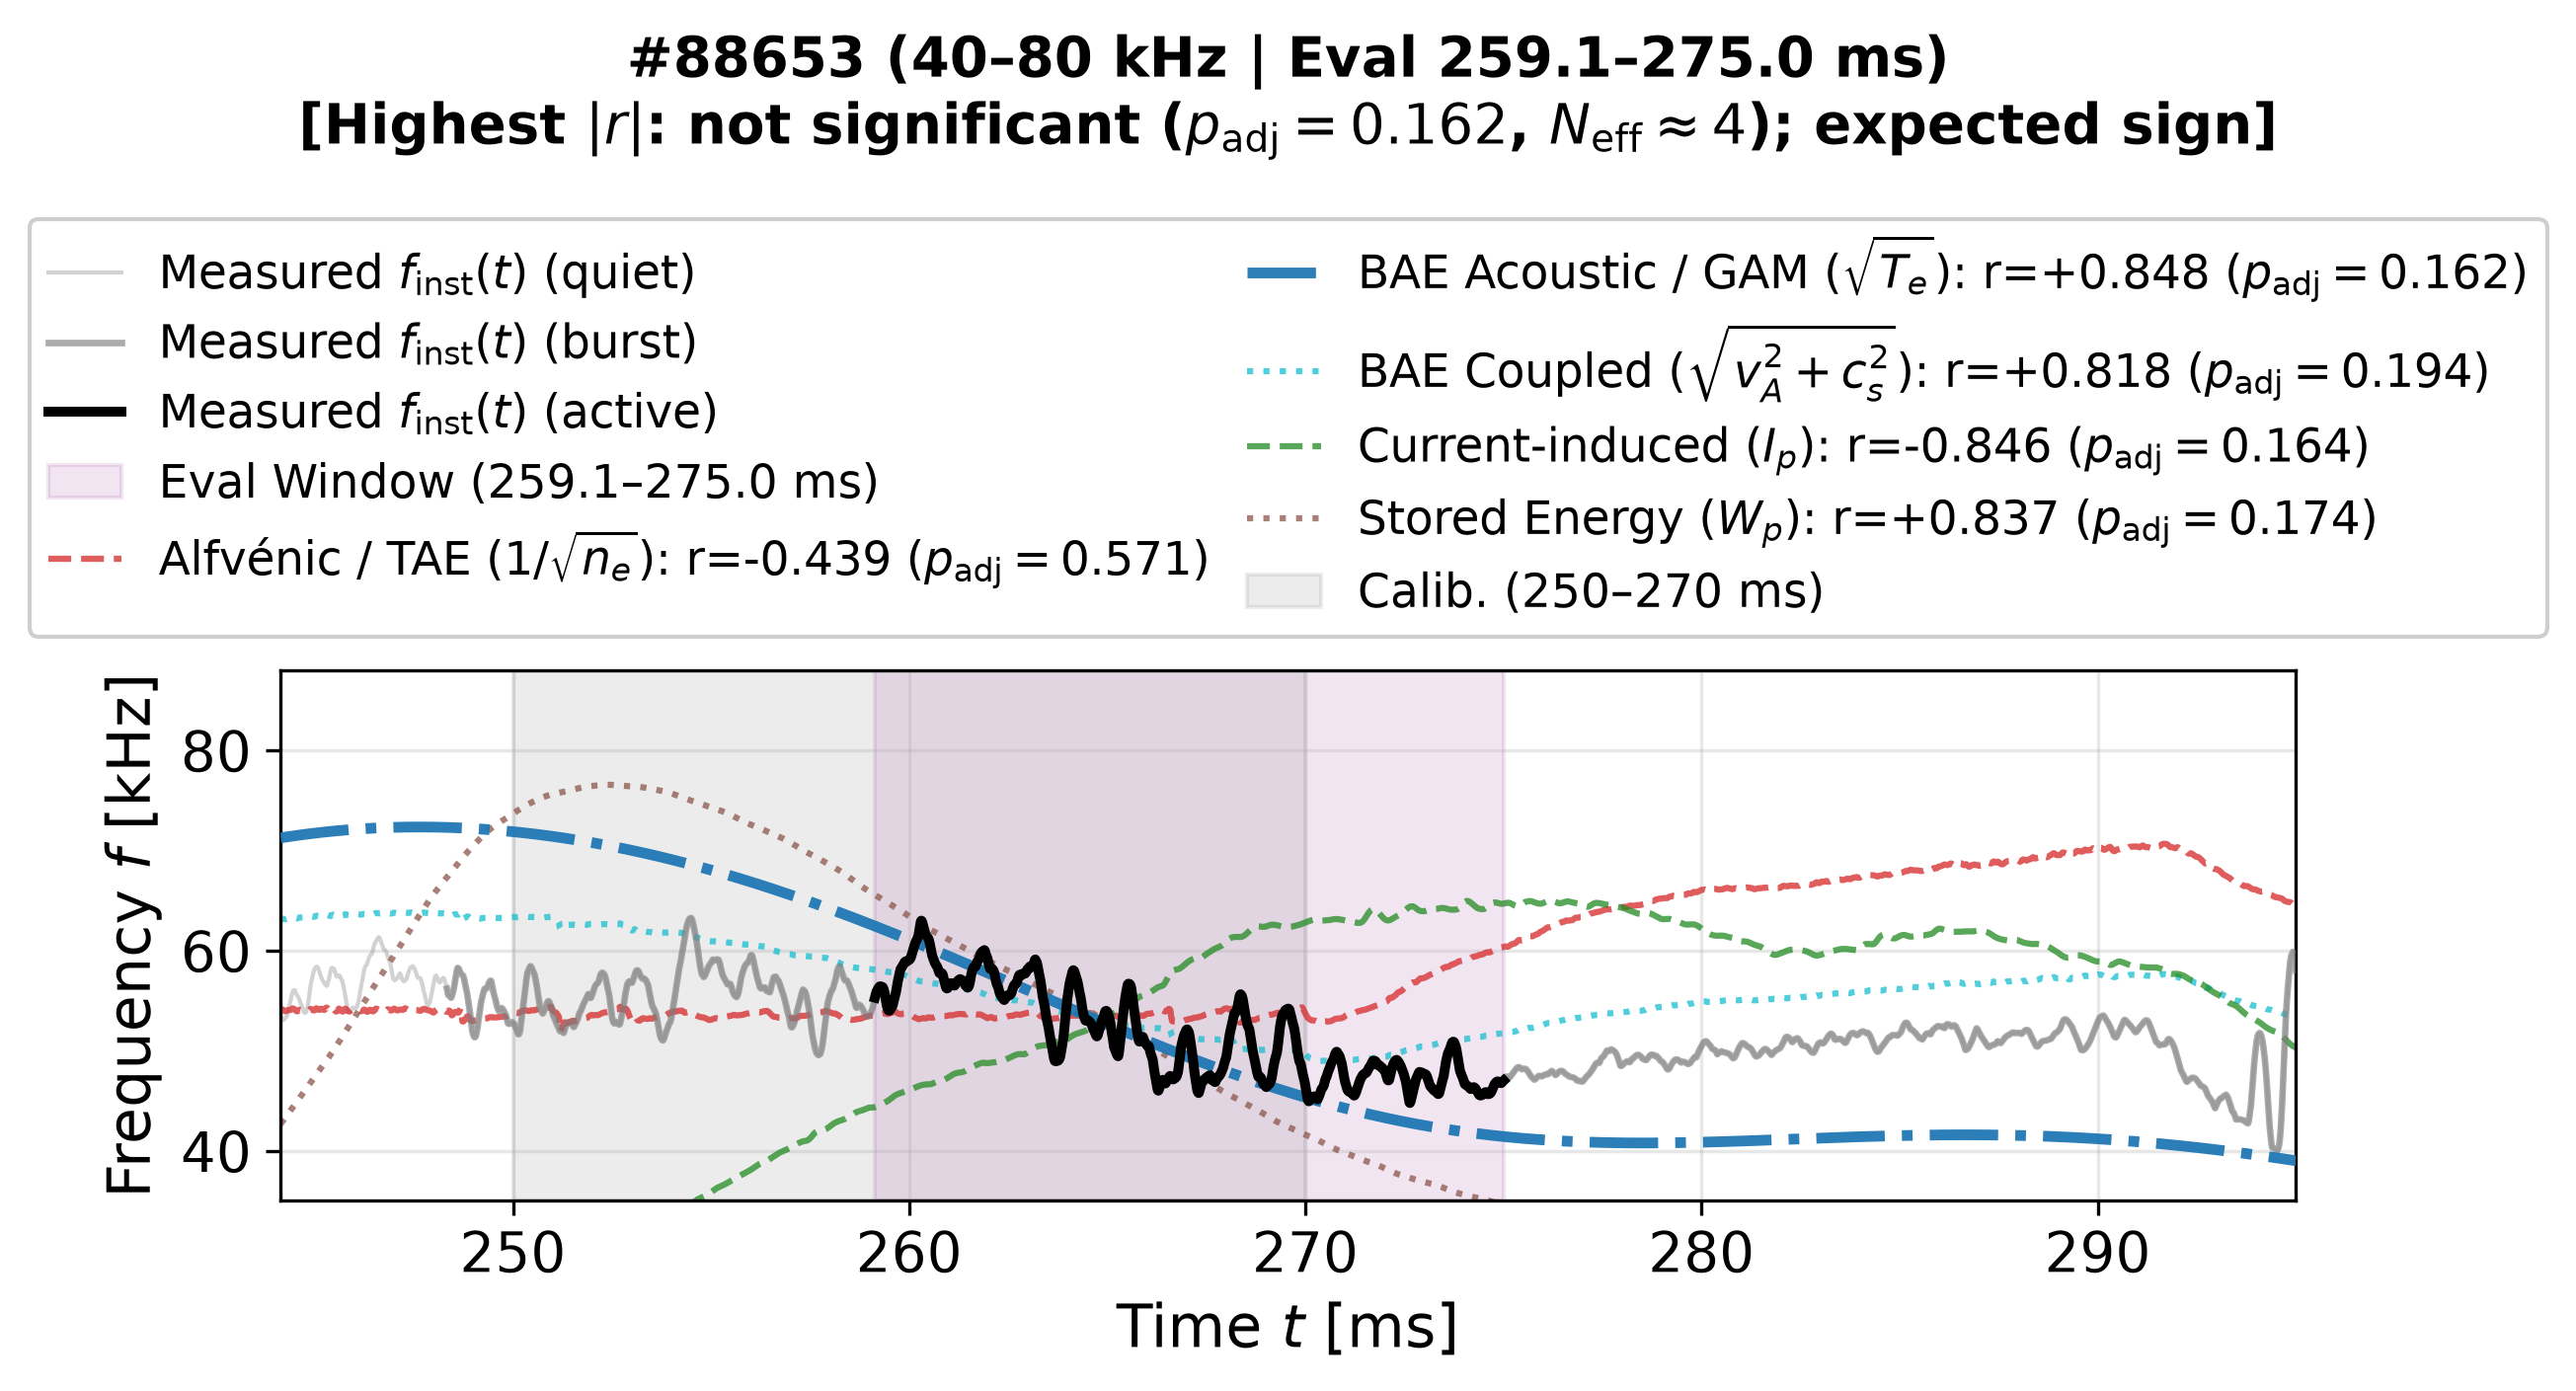
\includegraphics[width=0.92\textwidth]{Images/obj2_dynamics_and_structure/panels/mhd_analysis_objective2_heating_88653_40_80kHz_panel4_energetic_particle_mode_identification_m.png}
  \caption[Secondary mode frequency response to candidate scaling models]{Secondary mode ($40\text{--}80~\mathrm{kHz}$) frequency versus $30~\mathrm{Hz}$ LPF scaling models ($259.1\text{--}275.0~\mathrm{ms}$, \#88653).}
  \label{fig:obj2_epm_models_secondary}
\end{figure}

Figures~\ref{fig:obj2_epm_models_primary} and~\ref{fig:obj2_epm_models_secondary} compared primary ($80\text{--}120~\mathrm{kHz}$) and secondary ($40\text{--}80~\mathrm{kHz}$) frequency evolution in \#88653 against the five time-varying scaling models (calibrated on $250.0\text{--}270.0~\mathrm{ms}$) evaluated over $259.1\text{--}275.0~\mathrm{ms}$. Flat-top NBI beam scalings remained constant across this interval, while BAE traces used $30~\mathrm{Hz}$ SOS LPF smoothing. Filtering out ${\sim}800~\mathrm{Hz}$ sawtooth noise prevented sign-inversion artifacts and yielded positive acoustic tendencies for the primary mode: BAE Coupled ($\sqrt{v_A^2+c_s^2}$, $r = +0.545$, $p_{\mathrm{adj}} = 0.139$, $N_{\mathrm{eff}} \approx 9$) and BAE Acoustic ($\sqrt{T_e}$, $r = +0.392$, $p_{\mathrm{adj}} = 0.309$). In the secondary band, BAE Acoustic ranked highest ($r = +0.848$, $p_{\mathrm{adj}} = 0.162$), followed closely by current-induced shear shift ($r = -0.846$, $p_{\mathrm{adj}} = 0.164$) and $W_p$ ($r = +0.837$). This pointed to a candidate BAE or $\Delta I_p$-shifted acoustic mode. In replicate \#88654 ($248.3\text{--}268.4~\mathrm{ms}$, Table~\ref{tab:obj2_both_shots}), $W_p$ ranked first in both primary ($r = +0.604$, $p_{\mathrm{adj}} = 0.099$; BAE Coupled $+0.550$, BAE Acoustic $+0.546$) and secondary bands ($r = +0.343$, $p_{\mathrm{adj}} = 0.157$). Because no scaling achieved $|r| > 0.70$ at $p_{\mathrm{adj}} < 0.05$ and local $\iota/2\pi$ profiles were unavailable, individual weights remained \emph{suggestive}; as justified in Section~\ref{subsubsec:method_scaling}, small-$N_{\mathrm{eff}}$ curves ($N_{\mathrm{eff}} \approx 4.0\text{--}8.9$) were retained solely for exploratory physical ranking while reported as non-significant, and their positive acoustic compressibility scaling agreed with ECH/NBI-heated BAE and EPM trends~\cite{Zhong2024,Varela2015,Varela2023,Adulsiriswad_2024,Yamamoto_2020}.


\subsection{Objective 3 -- Nonlinear Three-Wave Coupling (Bicoherence)}
\label{subsec:obj3}

\subsubsection{General Search: Map Maxima and Reference Windows}
\label{subsubsec:obj3_maps}
The general search scanned the entire $(f_1, f_2)$ plane of each heated window to locate $\max b^2$. Because domain-wide maxima inflated extreme statistics by chance, raw peaks required calibration against a reference distribution. Here, the reference set spanned $33$ contiguous $7.936~\mathrm{ms}$ windows starting at $150.0~\mathrm{ms}$ (with linear detrending over $5\text{--}100~\mathrm{kHz}$, Figure~\ref{fig:obj3_control_windows}): $10$ overlapped NBI heating and $23$ lay outside ($2$ ohmic, $6$ ECH-only, $14$ post-NBI, plus $1$ straddling ECH turn-on), forming a mixed-regime reference rather than an unheated null.

\begin{figure}[htbp]
  \centering
  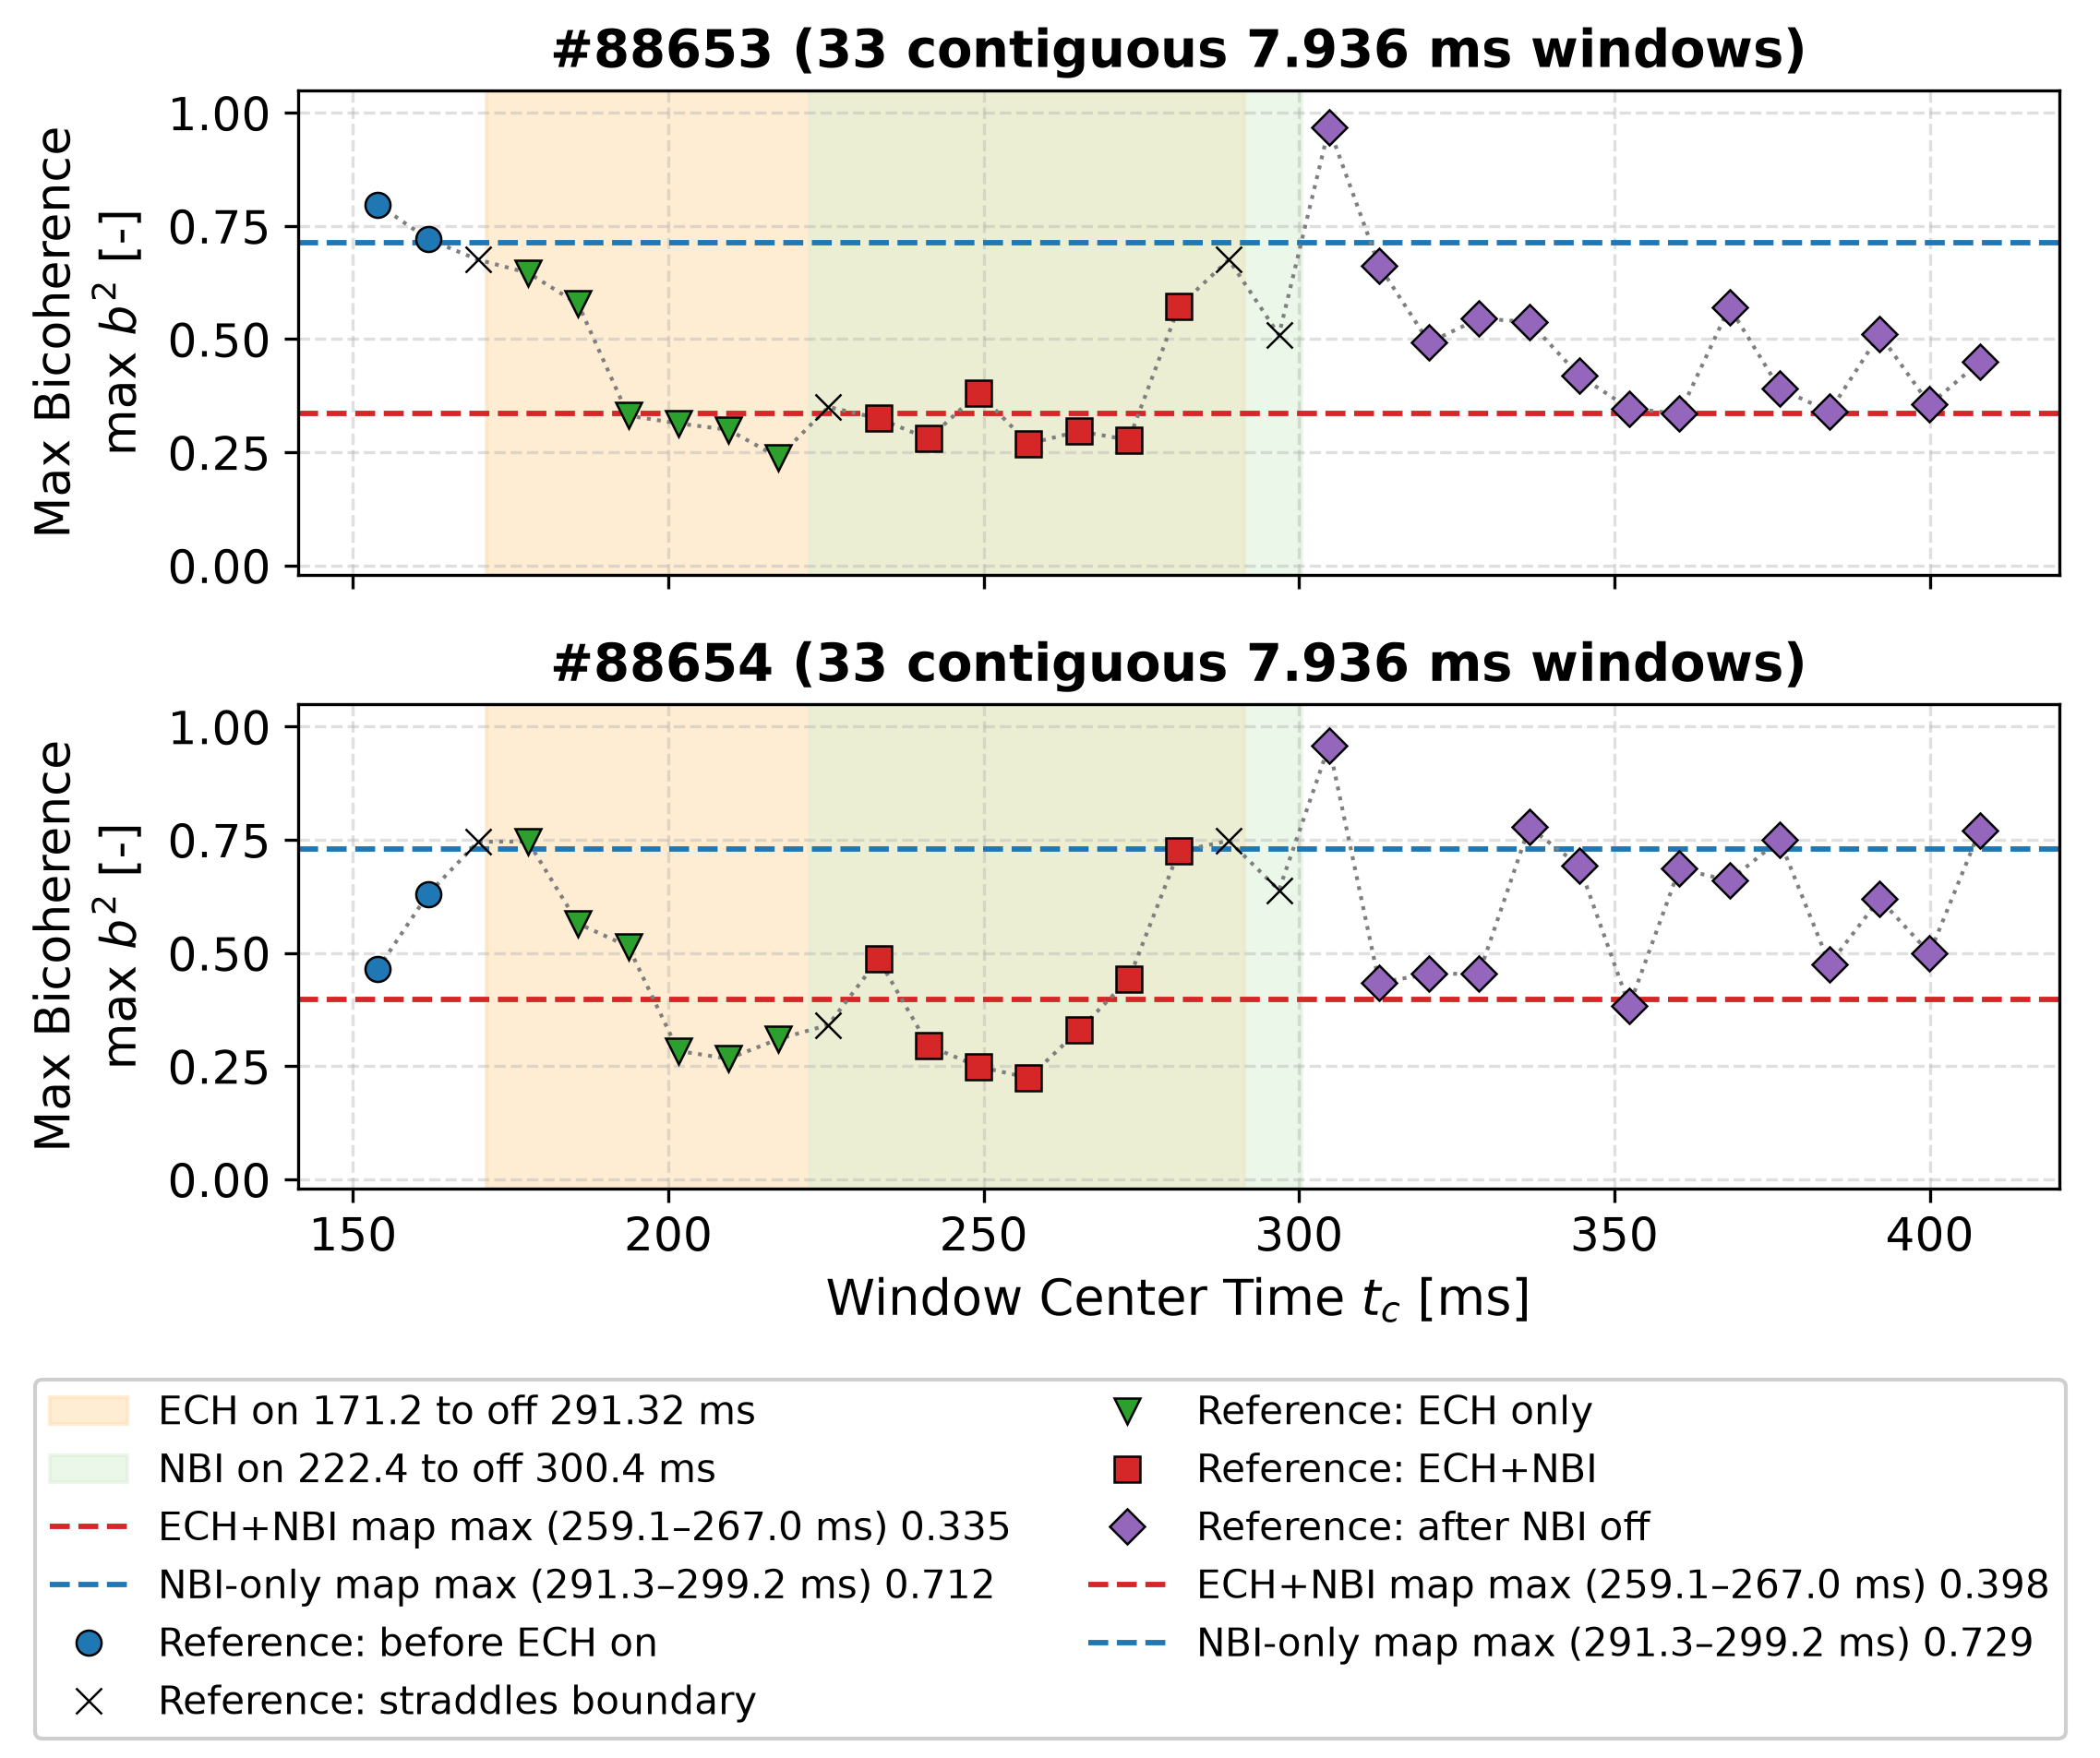
\includegraphics[width=0.75\textwidth]{Images/obj3_nonlinear_coupling/fig_control_windows_v2.png}
  \caption[Distribution of maximum squared bicoherence across reference windows]{Maximum $b^2$ ($5\text{--}100~\mathrm{kHz}$) across $33$ reference windows versus heated map maxima (dashed) for \#88653 and \#88654.}
  \label{fig:obj3_control_windows}
\end{figure}

\begin{figure}[htbp]
  \centering
  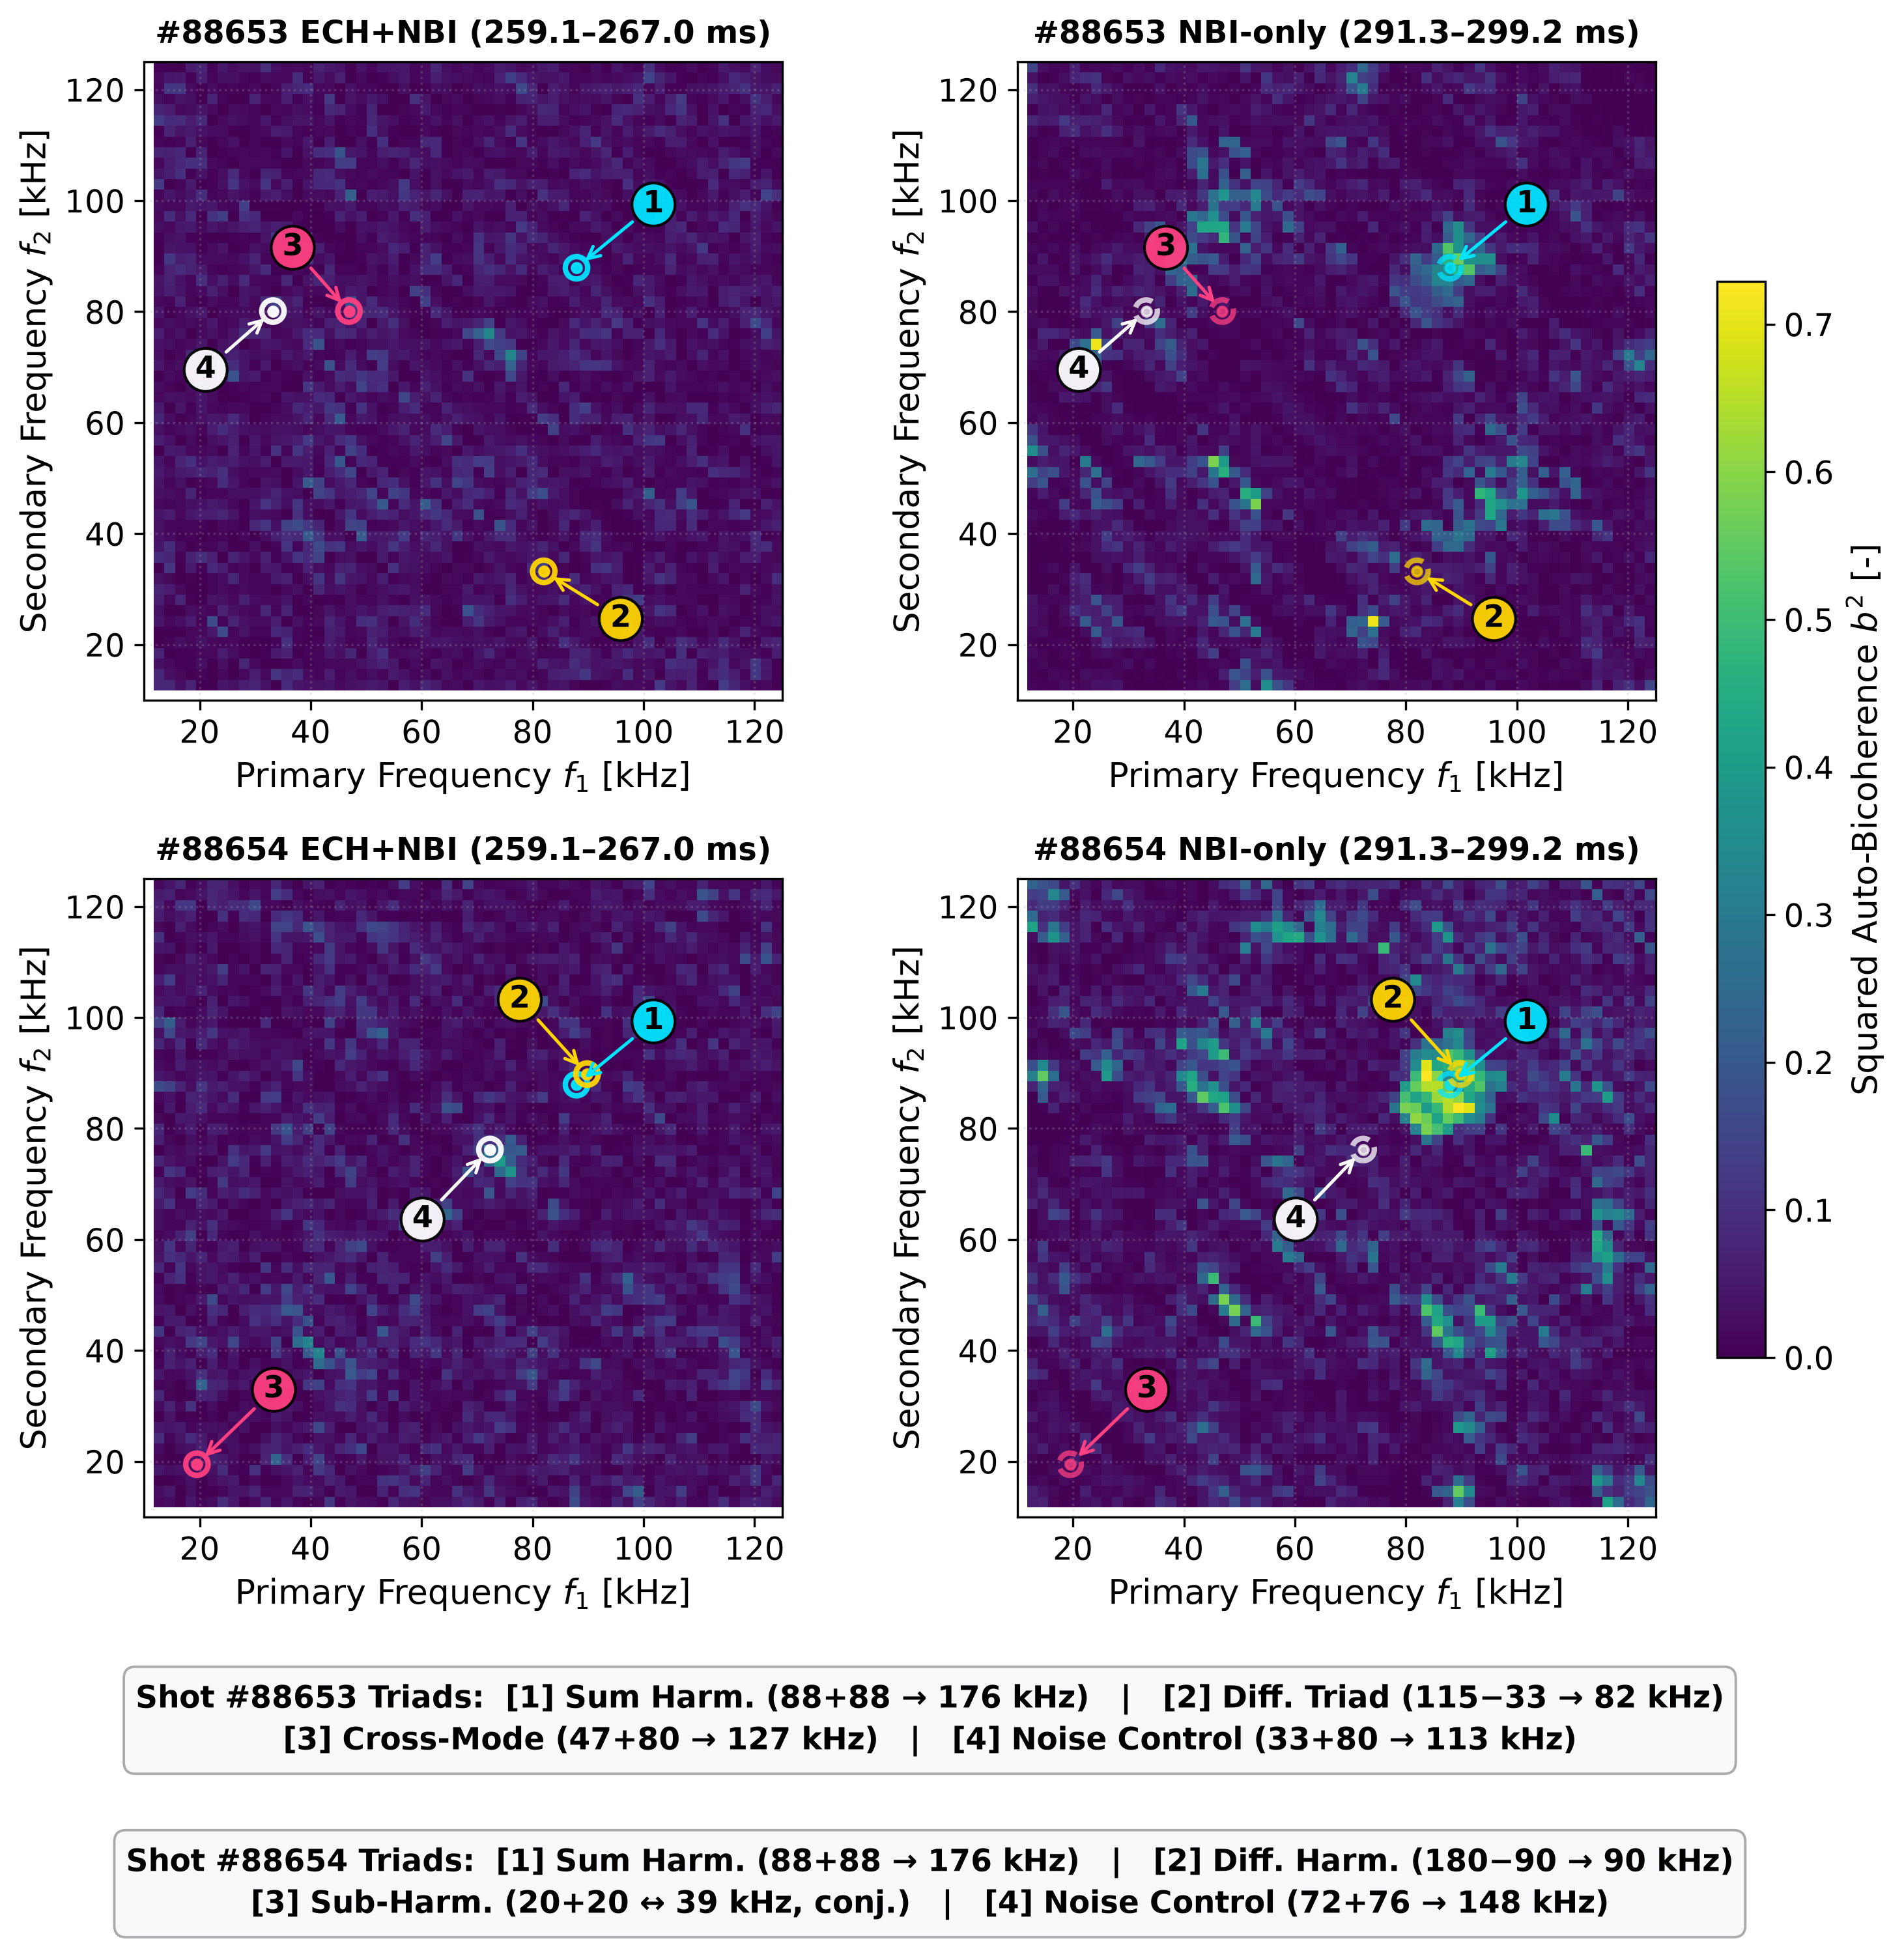
\includegraphics[width=0.88\textwidth]{Images/obj3_nonlinear_coupling/fig_bicoherence_maps_both_shots.png}
  \caption[Bicoherence maps, both shots]{Corrected MP1 $b^2(f_1, f_2)$ maps in $\mathrm{ECH}+\mathrm{NBI}$ and $\mathrm{NBI}$-only phases ($10\text{--}125~\mathrm{kHz}$) with triad markers [1]--[4].}
  \label{fig:bicoh_maps_both}
\end{figure}
Figures~\ref{fig:obj3_control_windows} and~\ref{fig:bicoh_maps_both} and Table~\ref{tab:bicoherence_maps} compared MP1 $b^2(f_1, f_2)$ in the $\mathrm{ECH}+\mathrm{NBI}$ ($259.1\text{--}267.0~\mathrm{ms}$) and $\mathrm{NBI}$-only ($291.3\text{--}299.2~\mathrm{ms}$) $7.936~\mathrm{ms}$ slices ($30$ segments) against the $33$ reference windows (with map markers [1]--[4] identifying the convergence-test primary harmonic, difference or conjugate triad, cross/sub-harmonic coupling, and noise baseline). Although $\mathrm{d}W_p/\mathrm{d}t$ regression was not performed directly, these windows evaluated nonlinear coupling inside the stored-energy regimes of Section~\ref{subsubsec:obj1_ech_off}. Over identical $7936$-sample slices, full-quadrant maxima in Figure~\ref{fig:bicoh_maps_both} matched detrended $5\text{--}100~\mathrm{kHz}$ maxima in Table~\ref{tab:bicoherence_maps} within $10^{-5}$. In $\mathrm{ECH}+\mathrm{NBI}$, map maxima ($0.335$ in \#88653; $0.398$ in \#88654) were exceeded by $23/33$ ($18/23$ non-overlapping) and $24/33$ ($19/23$) reference windows, respectively. In $\mathrm{NBI}$-only, maxima reached $0.712$ (\#88653, exceeded by $3/33$) and $0.729$ (\#88654, exceeded by $7/33$) from off-target peaks near $(23.4, 74.2)$ and $(84.0, 89.8)~\mathrm{kHz}$. Because domain maxima inflated false positives, $259.1~\mathrm{ms}$ overlapped the $261.1~\mathrm{ms}$ reference window, and reference windows mixed heating phases, raw map maxima remained \emph{inconclusive} alone.


\begin{table}[H]
\centering
\small
\caption[Bicoherence map maxima in heated and reference windows]{Bicoherence map maxima in heated and reference windows.}
\label{tab:bicoherence_maps}
\sbox0{%
\begin{tabular}{llcccc}
\toprule
Shot & Window type & Window (ms) & Map max $b^2$ (-) & Reference windows above / 33 & Reference windows above / 23 \\
\midrule
\#88653 & ECH+NBI & 259.1--267.0 & 0.335 & 23/33 & 18/23 \\
\#88653 & NBI-only & 291.3--299.2 & 0.712 & 3/33 & 3/23 \\
\#88653 & Reference windows & -- & median 0.419 [0.239, 0.967] & $N=33$ & median 0.492, $N=23$ \\
\#88654 & ECH+NBI & 259.1--267.0 & 0.398 & 24/33 & 19/23 \\
\#88654 & NBI-only & 291.3--299.2 & 0.729 & 7/33 & 6/23 \\
\#88654 & Reference windows & -- & median 0.499 [0.224, 0.958] & $N=33$ & median 0.565, $N=23$ \\
\bottomrule
\end{tabular}}
\ifdim\wd0>\textwidth\resizebox{\textwidth}{!}{\usebox0}\else\usebox0\fi
\par\smallskip{\footnotesize Strict comparison ($>$); bracketed values denote min--max range, not uncertainties. Reference set: 33 contiguous 7.936~ms windows from 150~ms (23 excluding NBI overlap; not a heating-free null).}
\end{table}


\subsubsection{Split-Sample General Search and Convergence Analysis}
\label{subsubsec:obj3_convergence}
To test whether elevated bicoherence represented genuine three-wave coupling rather than finite-sample bias, candidate peaks over $11.7\text{--}99.6~\mathrm{kHz}$ ($f_1 \le f_2$) were selected on selection segments and evaluated inside the $\mathrm{ECH}+\mathrm{NBI}$ window ($259.1\text{--}291.2~\mathrm{ms}$) across eight sub-ensemble counts $K$ ($500$ random $K$-segment subsets without replacement) on disjoint estimation blocks ($N_{\mathrm{est}}=40$ estimation segments in \#88653; $N=124$ segments in \#88654; Figure~\ref{fig:bicoh_general_search}). Extrapolating $b^2(K) = b_0 + C/K$ to $1/K \to 0$ isolated the asymptotic intercept $b_0$, and each cell was checked unpooled across all segments of the corresponding \#88654 window (Table~\ref{tab:convergence_general}).

\begin{figure}[H]
  \centering
  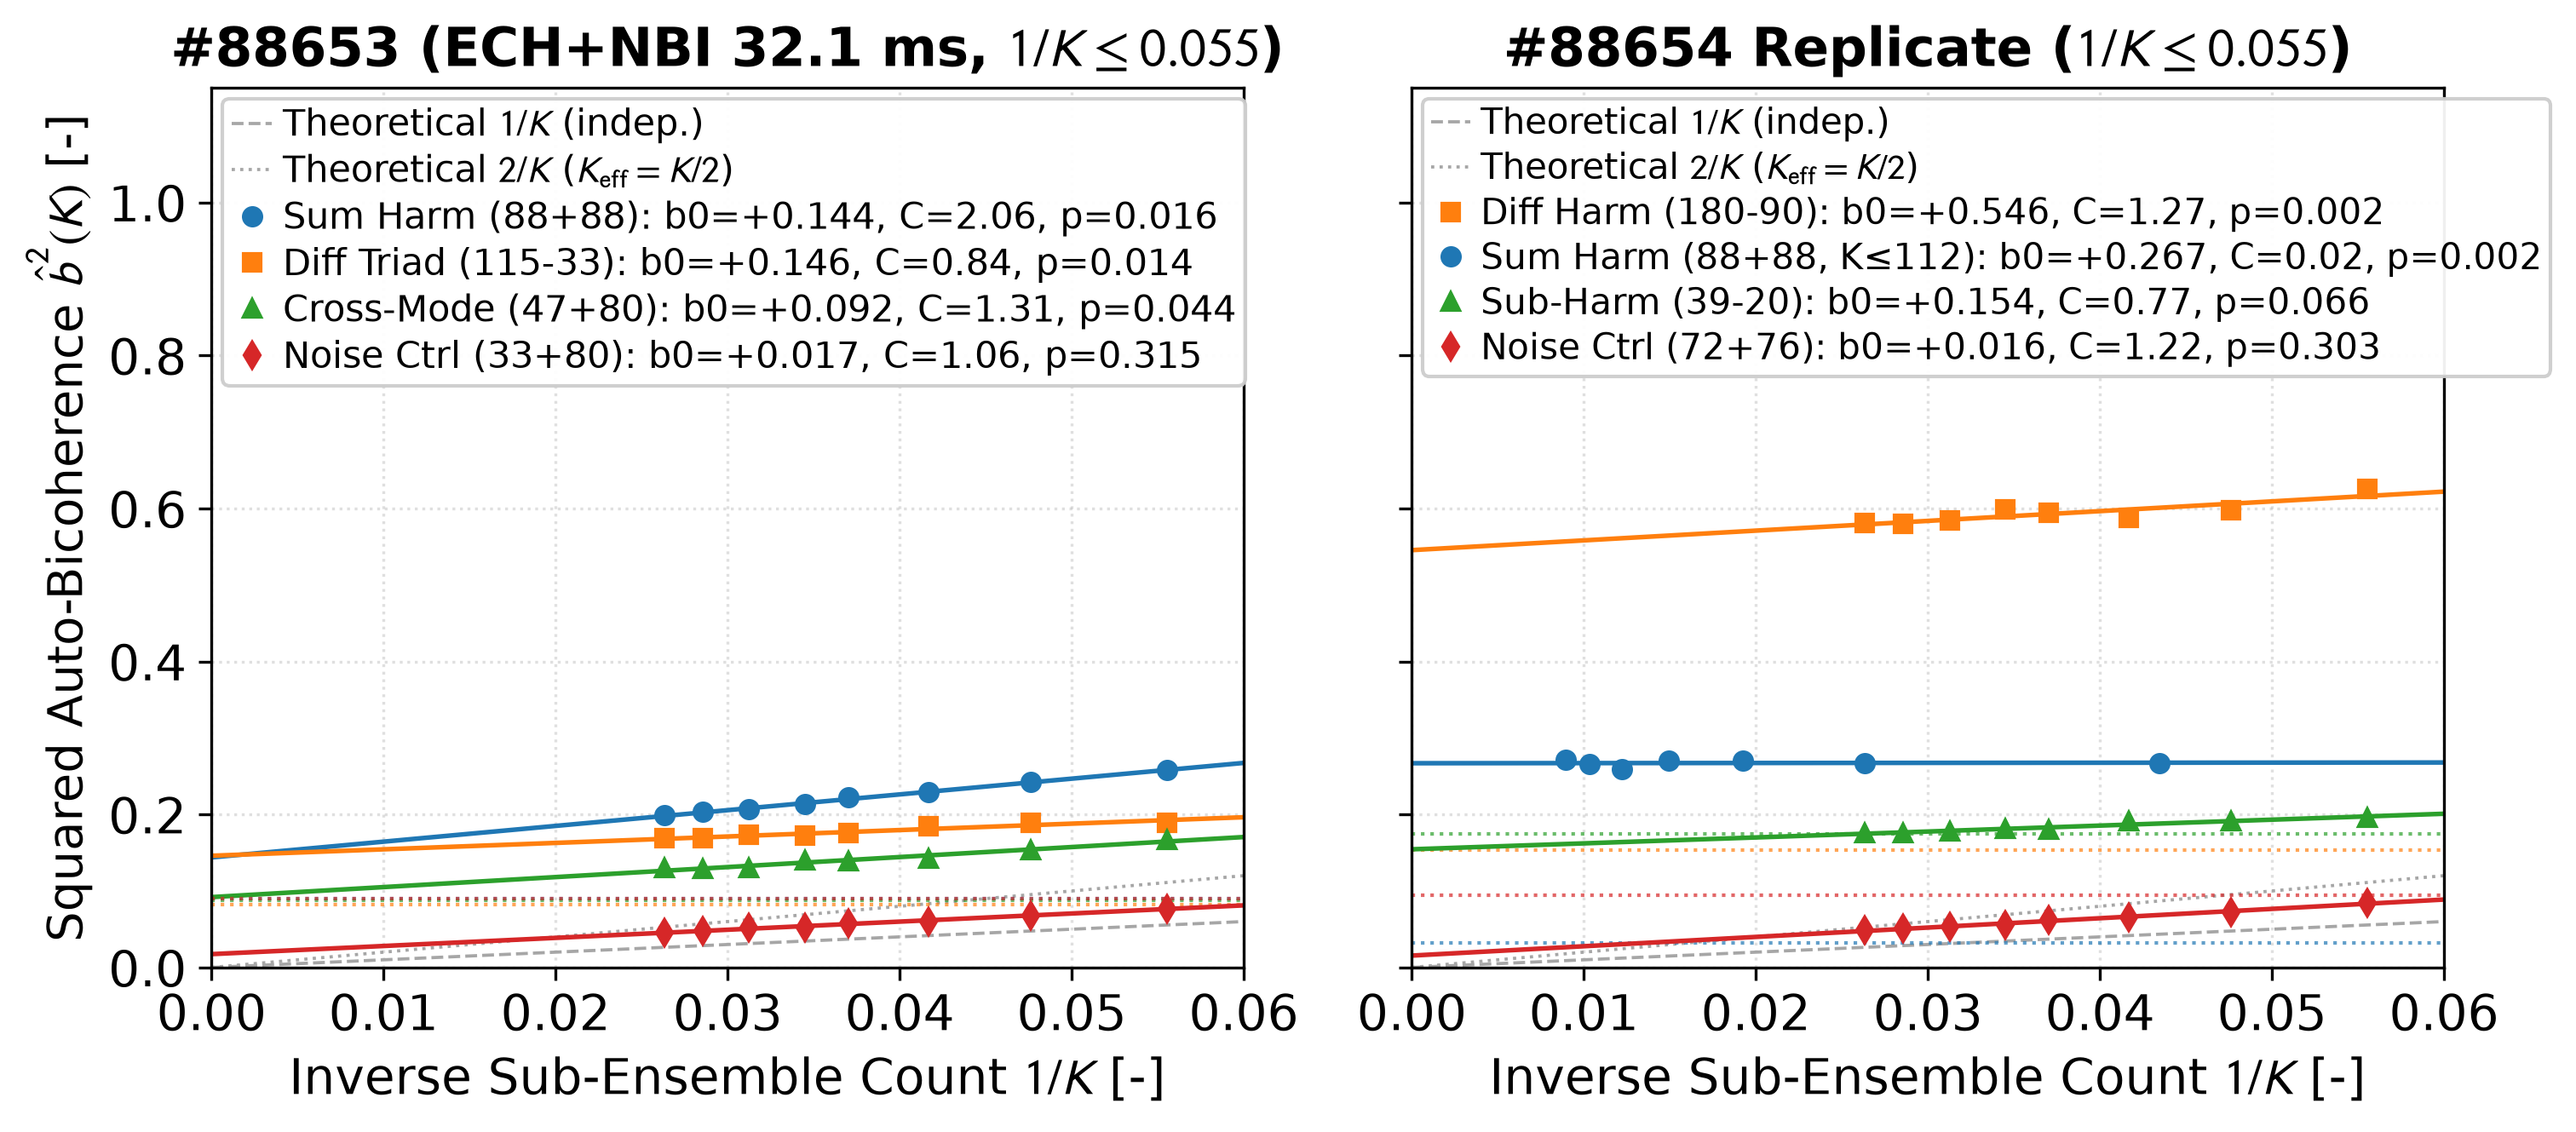
\includegraphics[width=0.90\textwidth]{Images/obj3_nonlinear_coupling/fig_convergence_cumulative_v3_general.png}
  \caption[General search: asymptotic convergence of the strongest peaks in both shots]{Asymptotic $b^2(K)$ convergence ($1/K \le 0.055$) in $\mathrm{ECH}+\mathrm{NBI}$ for shot \#88653 (left) and replicate \#88654 (right).}
  \label{fig:bicoh_general_search}
\end{figure}
\begin{table}[H]
\centering
\footnotesize
\linespread{0.91}\selectfont
\setlength{\tabcolsep}{2.95pt}
\setlength{\aboverulesep}{2pt}
\setlength{\belowrulesep}{2pt}
\renewcommand{\arraystretch}{0.92}
\caption[Asymptotic bicoherence convergence in the ECH+NBI window]{Asymptotic bicoherence convergence in the ECH+NBI window.}
\label{tab:convergence_general}
\begin{tabular}{@{}l >{\raggedright\arraybackslash}m{3.00cm} >{\centering\arraybackslash}m{3.32cm} c c c >{\raggedright\arraybackslash}m{3.68cm}@{}}
\toprule
Discharge & \shortstack[l]{Triad\\Type} & \shortstack{$f_1, f_2 \to f_3$\\(kHz)} & \shortstack{Intercept\\$b_0$ (-)} & \shortstack{Slope\\$C$ (-)} & \shortstack{Surrogate\\$p_{\rm surr}$ (-)} & \shortstack[l]{Validation Status\\($p < 0.05$)} \\
\midrule
\#88653 & Primary Sum Harmonic & $87.9 + 87.9 \to 175.8$ & $+0.144$ & $2.06$ & $0.016$ & Validated ($2/K$ overlap scaling) \\
\#88653 & Difference Triad & $115.2 - 33.2 \to 82.0$ & $+0.146$ & $0.84$ & $0.014$ & Validated (Inter-mode coupling) \\
\#88653 & Cross-Mode Interaction & $46.9 + 80.1 \to 127.0$ & $+0.092$ & $1.31$ & $0.044$ & Validated (Secondary-\newline to-primary flank) \\
\#88653 & Noise Contrast Baseline & $33.2 + 80.1 \to 113.3$ & $+0.017$ & $1.06$ & $0.315$ & Negative Control ($1/K \to 0$) \\
\midrule
\#88654 & Primary Harmonic\newline (Diff./Conj.) & $(89.8, 89.8) \leftrightarrow 179.7$\newline $(179.7\!-\!89.8\!\to\!89.8)$ & $+0.546$ & $1.27$ & $0.002$ & Validated (Adjacent-bin\newline conjugate replicate) \\
\#88654 & Primary Sum Harmonic & $87.9 + 87.9 \to 175.8$ & $+0.267$ & $0.02$ & $0.002$ & Validated (Cross-shot\newline harmonic replicate) \\
\#88654 & Sub-Harmonic Triad & $39.1 - 19.5 \to 19.5$ & $+0.154$ & $0.77$ & $0.066$ & Candidate (Marginal significance) \\
\#88654 & Noise Contrast Baseline & $72.3 + 76.2 \to 148.4$ & $+0.016$ & $1.22$ & $0.303$ & Negative Control ($1/K \to 0$) \\
\bottomrule
\end{tabular}
\par\vspace{2pt}\noindent\parbox{\textwidth}{\footnotesize ECH+NBI window ($259.1\text{--}291.2~\mathrm{ms}$), asymptotic regime $1/K \le 0.055$ ($K \ge 18$); \#88653 ($N_{\mathrm{est}}=40$), \#88654 ($N=124$). Mean of 500 random sub-ensembles without replacement ($95\,\%$ bounds $[q_{2.5}, q_{97.5}]$ reflect finite-$K$ sub-ensemble dispersion, whereas $p_{\rm surr}$ tests mean $b_0$ vs.\ 500 phase-randomized surrogates). In \#88654, marker~[2] at $(f_1, f_2) = (89.8, 89.8)~\mathrm{kHz}$ (adjacent to $(87.9, 87.9)~\mathrm{kHz}$ within the scanned $f_1, f_2 \in [11.7, 99.6]~\mathrm{kHz}$ plane) couples the fundamental $89.8~\mathrm{kHz}$ mode with its second harmonic at $f_1 + f_2 = 179.7~\mathrm{kHz}$---equivalent by Hermitian conjugate symmetry to $179.7 - 89.8 \to 89.8~\mathrm{kHz}$---marking an adjacent-bin conjugate realization of the same primary self-harmonic steepening over $N=124$ rather than an independent triad. The brief $8.7~\mathrm{ms}$ NBI-only interval ($291.3\text{--}300.0~\mathrm{ms}$, $N_{\mathrm{seg}}=32$) yielded only $2$ estimation units ($<6$ required) and was \emph{untestable} in both \#88653 and \#88654.}
\end{table}

In Figure~\ref{fig:bicoh_general_search} (showing subset means against theoretical $1/K$ and $2/K$ lines, dotted horizontal $95~\%$ surrogate nulls, and legend parameters $(b_0, C, p_{\mathrm{surr}})$) and Table~\ref{tab:convergence_general}, restricting fits to $1/K \le 0.055$ ($K \ge 18$, including $K \le 112$ over $N=124$ for the \#88654 sum harmonic) eliminated small-ensemble curvature bias and yielded tight linear regressions ($R^2 \ge 0.96\text{--}0.99$). Three candidate triads in \#88653 cleared the $500$-surrogate null ($p_{\mathrm{surr}} < 0.05$). First, primary-mode self-harmonic steepening (marker~[1], $(87.9, 87.9) ~\mathrm{kHz}\to 175.8~\mathrm{kHz}$) reached $b_0 = +0.144$ ($p_{\mathrm{surr}} = 0.0160$, testing the mean intercept against $500$ phase-randomized surrogates) along the $2/K$ overlap slope ($C = +2.06$), with finite-$K$ dispersion $[q_{2.5}, q_{97.5}] = [-0.029, +0.320]$. Second, a difference triad (marker~[2], $(115.2, -33.2)~\mathrm{kHz}\to 82.0~\mathrm{kHz}$) converged to $b_0 = +0.146$ ($p_{\mathrm{surr}} = 0.0140$). Third, a sum triad coupling the secondary mode to the primary flank (marker~[3], $(46.9, 80.1)~\mathrm{kHz}\to 127.0~\mathrm{kHz}$) converged to $b_0 = +0.092$ ($p_{\mathrm{surr}} = 0.0439$). Conversely, the off-diagonal noise baseline (marker~[4], $(33.2, 80.1)\to 113.3~\mathrm{kHz}$) followed the theoretical $1/K$ slope ($C = +1.06$) directly to zero ($b_0 = +0.017 \approx 0.000$, $p_{\mathrm{surr}} = 0.3154$).

In replicate \#88654 ($N = 124$ segments), primary harmonic steepening remained validated in both the conjugate difference ($(179.7, -89.8)~\mathrm{kHz}\to 89.8~\mathrm{kHz}$, $b_0 = +0.546$, $p_{\mathrm{surr}} = 0.0020$) and sum channels ($(87.9, 87.9)~\mathrm{kHz}\to 175.8~\mathrm{kHz}$, $b_0 = +0.267$, $p_{\mathrm{surr}} = 0.0020$). Specifically, in \#88654 (scanned plane $f_1, f_2 \in [11.7, 99.6]~\mathrm{kHz}$), marker~[2] at $(89.8, 89.8)~\mathrm{kHz}$ (adjacent to $(87.9, 87.9)~\mathrm{kHz}$) coupled the $89.8~\mathrm{kHz}$ fundamental with $f_1+f_2=179.7~\mathrm{kHz}$---conjugate-equivalent to $179.7~\mathrm{kHz} -89.8 ~\mathrm{kHz}\to 89.8~\mathrm{kHz}$ in Table~\ref{tab:convergence_general}---marking the same self-harmonic steepening, while marker~[3] at $(19.5, 19.5)~\mathrm{kHz}$ corresponded via conjugate symmetry to the marginal sub-harmonic triad $39.1~\mathrm{kHz} -19.5~\mathrm{kHz}\to 19.5~\mathrm{kHz}$ ($b_0=+0.154$, $p_{\mathrm{surr}}=0.066$). Meanwhile, its noise baseline (marker~[4], $72.3 ~\mathrm{kHz} + 76.2 ~\mathrm{kHz}\to 148.4~\mathrm{kHz}$ in Table~\ref{tab:convergence_general}) decayed along $1/K$ directly to zero ($b_0 = +0.016$, $p_{\mathrm{surr}} = 0.3034$). In contrast, the brief $8.7~\mathrm{ms}$ $\mathrm{NBI}$-only phase ($291.3\text{--}300.0~\mathrm{ms}$, $N_{\mathrm{seg}} = 32$) yielded only $2$ disjoint estimation blocks, below the $6$-block minimum required for unbiased split-sample regression, and was therefore classified as \emph{untestable} in both \#88653 and \#88654.

Whereas preliminary single-window evaluations using the uncorrected \texttt{jpack} estimator appeared inconclusive due to the one-bin \texttt{np.roll} offset and finite-sample bias, rectifying the index lookup and extrapolating $b^2(K)$ over $1/K \le 0.055$ cleanly isolated this quadratic phase locking. Consistent with bispectral theory~\cite{KimPowers1979} and helical/tokamak studies~\cite{Kin2025,Miyashita2025,Hou2019}, positive asymptotic intercepts ($b_0 > 0$) versus $1/K \to 0$ baseline decay confirmed genuine quadratic phase locking among the primary mode, its second harmonic, and lower-frequency fluctuations.

\subsection[Integrated Physical Discussion and Quantitative Literature Contrast]{Integrated Physical Discussion and Quantitative\\ Literature Contrast}
\label{subsec:integrated_discussion}
A first-principles order-of-magnitude Alfv\'enic scaling analysis supports the physical assignment of both coherent frequency bands in Heliotron~J. For standard parameters ($B_0 = 1.25~\mathrm{T}$, $n_e \approx 0.6\text{--}1.0 \times 10^{19}~\mathrm{m^{-3}}$, $R_0 = 1.2~\mathrm{m}$, $\iota/2\pi \approx 0.56$), Eq.~(\ref{eqn:alfven}) yields $v_A \approx 6.1\text{--}7.9 \times 10^6~\mathrm{m/s}$ ($f_{\mathrm{TAE}} = (\iota/2\pi)v_A/(4\pi R_0) \approx 226\text{--}292~\mathrm{kHz}$) for pure deuterium ($m_i = 2 m_p$), and $v_A \approx 6.1\text{--}11.2 \times 10^6~\mathrm{m/s}$ ($f_{\mathrm{TAE}} \approx 226\text{--}412~\mathrm{kHz}$) across mixed hydrogen--deuterium NBI plasmas ($m_{\mathrm{eff}} \approx 1.0\text{--}2.0\,m_p$). Both observed bands ($40\text{--}50~\mathrm{kHz}$ and $86\text{--}90~\mathrm{kHz}$) therefore lie well below the TAE continuum gap ($> 220~\mathrm{kHz}$), ruling out a standard gap TAE and pointing instead to lower-frequency BAE or resonant EPM branches. Evaluating the BAE/GAM acoustic baseline in Eq.~(\ref{eqn:f_bae_baseline}),
\begin{equation}
\label{eqn:f_bae_baseline}
f_{\mathrm{BAE}} \approx \frac{1}{2\pi R_0}\sqrt{\frac{2 k_B T_i}{m_i}\left(\frac{7}{4} + \frac{T_e}{T_i}\right)},
\end{equation}
where $R_0$ is the major radius ($\mathrm{m}$), $k_B$ is the Boltzmann constant ($\mathrm{J/K}$), $m_i$ is the effective ion mass ($\mathrm{kg}$), and $T_e$ and $T_i$ are the core electron and ion temperatures ($\mathrm{K}$), for typical Heliotron~J core conditions under $\mathrm{ECH}+\mathrm{NBI}$ ($T_e \approx 0.3\text{--}0.8~\mathrm{keV}$, $T_i \approx 0.15\text{--}0.3~\mathrm{keV}$) yields an ion-acoustic speed $c_s = \sqrt{k_B T_e / m_i} \approx 1.2\text{--}2.0 \times 10^5~\mathrm{m/s}$ (pure $\mathrm{D}_2$) and $f_{\mathrm{BAE}} \approx 31\text{--}47~\mathrm{kHz}$ ($\approx 31\text{--}55~\mathrm{kHz}$ across $m_{\mathrm{eff}} \approx 1.5\text{--}2.0\,m_p$) in quantitative agreement with the observed $40\text{--}50~\mathrm{kHz}$ secondary mode (consistent with the Eq.~(\ref{eqn:gam}) $\sqrt{T_e}$ proxy because $\frac{7}{4}T_i + T_e$ is electron-dominated at $T_e > T_i$), while finite-$k_\parallel$ Alfv\'en--acoustic coupling ($\sqrt{v_A^2 k_\parallel^2 + \omega_{\mathrm{BAE}}^2}/(2\pi)$ for small effective $|k_\parallel R_0| \sim 0.04\text{--}0.12$) spans $80\text{--}100~\mathrm{kHz}$; because unshifted vacuum $|m(\iota/2\pi) - n| > 1$ for $m = +3$ and $n \equiv -1 \pmod 4$ at $\iota/2\pi \approx 0.56$, placing the $86\text{--}90~\mathrm{kHz}$ primary branch in this range points either to helical $M = 4$ sideband coupling or fast-ion resonant EPM drive (Eq.~(\ref{eqn:condition})). Contrasting these findings with prior Heliotron~J investigations highlights strong continuity alongside configuration-specific distinctions. Yamamoto \emph{et~al.}~\cite{Yamamoto_2020}, Varela \emph{et~al.}~\cite{Varela2023}, and Zhong \emph{et~al.}~\cite{Zhong2024} report NBI-driven core EPMs across $60\text{--}120~\mathrm{kHz}$ modulated by ECH/ECCD electron heating, matching the $86\text{--}90~\mathrm{kHz}$ ($m = +3$, $n \equiv -1 \pmod 4$) primary branch and the ECH-off sensitivity of the $40\text{--}50~\mathrm{kHz}$ secondary branch. Likewise, 3D gyrofluid simulations by Varela \emph{et~al.}~\cite{Varela2015} confirm that low-$n$ EPM/BAE drive tracks fast-ion pressure gradients inside the core-to-mid zone ($\rho \approx 0.29\text{--}0.47$). By contrast, Zang \emph{et~al.}~\cite{zang2019observation} observe an outer-gradient BAE/global Alfv\'en eigenmode (GAE)-band instability at $\rho = 0.86\text{--}0.91$ with $m \sim 6\text{--}8$. The modes isolated here peak deeper in the core ($\rho_{\mathrm{centroid}} \approx 0.38$, $m = +3$ and coexisting $m_1 = +1$ global / $m_2 = +12$ components). Furthermore, the outward ECE wavepacket group velocity ($v_{\mathrm{g},r} \approx +22$ to $+36~\mathrm{km/s}$) extends prior Heliotron~J fluctuation radiometry~\cite{luo2020measurement} to resolved core energy propagation. The asymptotic bicoherence intercepts ($b_0 = +0.092$ to $+0.546$) also align quantitatively with nonlinear mode--turbulence and Alfv\'enic couplings in Heliotron~J~\cite{Kin2025,Miyashita2025} and the HL-2A tokamak~\cite{Hou2019}. Table~\ref{tab:literature_contrast} synthesizes this quantitative benchmark against prior helical and tokamak studies.

\begin{table}[H]
  \centering
  \caption[Quantitative comparison between the present Heliotron~J study and prior literature]{Quantitative comparison between the present Heliotron~J study and prior literature.}
  \label{tab:literature_contrast}
  \footnotesize
  \setlength{\tabcolsep}{4pt}
  \renewcommand{\arraystretch}{1.18}
  \begin{tabular}{>{\raggedright\arraybackslash}p{0.19\textwidth}>{\raggedright\arraybackslash}p{0.20\textwidth}>{\raggedright\arraybackslash}p{0.25\textwidth}>{\raggedright\arraybackslash}p{0.28\textwidth}}
    \toprule
    \textbf{Study (Device)} & \textbf{Regime \& Diagnostics} & \textbf{Observed Mode \& Scaling} & \textbf{Key Benchmark Contrast} \\
    \midrule
    Yamamoto \emph{et~al.}~\cite{Yamamoto_2020} (Heliotron~J) & NBI + ECH/ECCD; Mirnov arrays & Core EPMs ($60\text{--}120~\mathrm{kHz}$); ECH/ECCD shift & Matches $86\text{--}90~\mathrm{kHz}$ ($m=+3$) band; extended here to 18-coil $\times$ 16-ECE mapping \\
    Zhong \emph{et~al.}~\cite{Zhong2024} \& Varela \emph{et~al.}~\cite{Varela2023} (Heliotron~J) & NBI + modulated ECH; Mirnov \& $W_p$ & Core EPM/BAE ($60\text{--}120~\mathrm{kHz}$); ECH-driven $\Delta f$ & Mirrors $-9.69~\mathrm{kHz}$ ECH-off step ($p_{\mathrm{surr}} = 0.004$); shown non-reducible to $n_e$ (explaining $\le 26.2~\%$ of $\Delta f$) \\
    Zang \emph{et~al.}~\cite{zang2019observation} (Heliotron~J) & NBI; Mirnov \& radial arrays & Outer BAE/GAE ($\rho = 0.86\text{--}0.91$, $m \sim 6\text{--}8$) & Modes here peak deeper ($\rho \approx 0.29\text{--}0.47$, centroid $0.38$) with $m=+3$ and $(+1, +12)$ \\
    Varela \emph{et~al.}~\cite{Varela2015,Varela2024} (Heliotron~J, TJ-II) & FAR3d 3D gyrofluid modeling & Low-$n$ core-to-mid EPM/BAE ($\nabla p_f$ drive) & Equilibrium drive zone matches measured $\rho \approx 0.29\text{--}0.47$ and $n \equiv -1 \pmod 4$ \\
    Luo \emph{et~al.}~\cite{luo2020measurement} \& Weir~\cite{Weir2019} (Heliotron~J) & 16-channel / correlation ECE ($57.5\text{--}72.5~\mathrm{GHz}$) & Internal $T_e$ fluctuation radiometry & Extended to inward carrier tilt ($\Delta\tau = -0.39$ to $-0.51~\mu\mathrm{s}$) vs. outward $v_{\mathrm{g},r} \approx +22$ to $+36~\mathrm{km/s}$ \\
    Kin \emph{et~al.}~\cite{Kin2025} \& Hou \emph{et~al.}~\cite{Hou2019} (Heliotron~J, HL-2A) & Higher-order auto-bicoherence $b^2$ & Nonlinear mode--turbulence / Alfv\'en coupling & Isolated via $1/K \to 0$ intercept ($b_0 = +0.092$ to $+0.546$, $p_{\mathrm{surr}} \le 0.0439$) vs. $O(1/K)$ null \\
    \textbf{Present work} (Heliotron~J, \#88653/4) & 18 Mirnov + 16 ECE + $W_p, I_p, n_e$; Python/NUDFT & Primary $86\text{--}90~\mathrm{kHz}$ ($m=+3$); secondary $40\text{--}50~\mathrm{kHz}$ & Rectified $1.953~\mathrm{kHz}$ \texttt{jpack} shift; Bartlett $N_{\mathrm{eff}}$, FDR-BH, and $500$-surrogate bounds \\
    \bottomrule
  \end{tabular}
\end{table}

From an experimental-design standpoint, evaluating the matched control-versus-perturbation pair (\#88653 primary and \#88654 unpooled replicate) avoids artificial sample pooling while retaining substantial within-discharge statistical power. Rather than treating $N = 2$ as an underpowered macro-sample, inference operates over $262\,144$ samples per $1~\mathrm{MHz}$ diagnostic trace, $18 \times 16 = 288$ cross-diagnostic coil--radiometer spatial pairs, $33$ contiguous empirical reference windows, and $80\text{--}124$ overlapping spectral segments per heating phase, all calibrated via Bartlett autocorrelation $N_{\mathrm{eff}}$, FDR-BH multiplicity control, and $500$ phase-randomized surrogates. Concurrently, negative partial correlations and non-significant dispersion $p_{\mathrm{adj}}$ define exact empirical sensitivity limits without overclaiming causality.

Synthesizing Objectives~1--3 establishes a unified, quantitatively bounded view of multi-diagnostic MHD behavior across heated Heliotron~J discharges. Objective~1 confirms that NBI fast ions destabilize core helical modes ($m = +3$ and $m_1 = +1$, $n \equiv -1 \pmod 4$) whose wavepackets propagate outward ($v_{\mathrm{g},r} \approx +22~\mathrm{km/s}$ to $+36~\mathrm{km/s}$). Across ECH switch-off, these modes persist with a $-9.69~\mathrm{kHz}$ secondary-centroid shift ($-9.86~\mathrm{kHz}$ in \#88654) and a $-54.3~\mathrm{kW}$ to $-81.1~\mathrm{kW}$ $\mathrm{d}W_p/\mathrm{d}t$ step ($-54.3~\mathrm{kW}$ to $-60.9~\mathrm{kW}$ in \#88653; $-68.3~\mathrm{kW}$ to $-81.1~\mathrm{kW}$ in \#88654) driven primarily by ECH power removal. Objective~2 evaluates lagged envelope correlations, showing that shared heating ramps ($N_{\mathrm{eff}} \approx 15.8\text{--}34.1$) yield near-zero step-controlled partial correlations. It also verifies a $30~\mathrm{Hz}$ LPF ECE relative thermal proxy (\texttt{ECE12FAST} core and \texttt{ECE9FAST} chord-integrated) and identifies positive, physically consistent (though statistically non-significant, $p_{\mathrm{adj}} = 0.099\text{--}0.162$) tendencies toward candidate $\sqrt{T_e}$ and $\sqrt{v_A^2 + c_s^2}$ BAE scalings. Objective~3 demonstrates that combined $\mathrm{ECH}+\mathrm{NBI}$ heating exhibits validated self-harmonic steepening ($87.9 + 87.9~\mathrm{kHz} \to 175.8~\mathrm{kHz}$, $b_0 > 0$, $p_{\mathrm{surr}} < 0.05$) and inter-mode phase locking against $500$ surrogates, separating true coupling from $O(1/K) \to 0$ noise.

These validated tools and findings provide concrete institutional value across both partner laboratories. At IAE, Kyoto University, the rectified \texttt{jpack} auto-bicoherence routine (\texttt{abicoh2\_\allowbreak corrected.py}, fixing the $1.953~\mathrm{kHz}$ one-bin shift) and automated \texttt{.json} and spectrogram mode-cataloging pipeline integrate directly into daily Heliotron~J campaign analysis to replace manual shot screening. Simultaneously, at PlasmaTEC, ITCR, these methods transfer directly to possible Mirnov and Langmuir probe diagnostics on the Stellarator of Costa Rica~1 (SCR-1) and spherical torus experiments. In particular, the NUDFT array decomposition, Bartlett $N_{\mathrm{eff}}$ auditing, and surrogate-calibrated $1/K$ bicoherence workflow isolate true couplings from finite-sample variance.
